%%%%%%%%%%%%%%%%%%%%%%%%%%%%%%%%%%%%%%%%%
% Journal Article
% LaTeX Template
% Version 2.0 (February 7, 2023)
%
% This template originates from:
% https://www.LaTeXTemplates.com
%
% Author:
% Vel (vel@latextemplates.com)
%
% License:
% CC BY-NC-SA 4.0 (https://creativecommons.org/licenses/by-nc-sa/4.0/)
%
% NOTE: The bibliography needs to be compiled using the biber engine.
%
% The previous LaPreprint version of this manuscript is kept in
% main_lapreprint.tex.
%
%%%%%%%%%%%%%%%%%%%%%%%%%%%%%%%%%%%%%%%%%

%----------------------------------------------------------------------------------------
%	PACKAGES AND OTHER DOCUMENT CONFIGURATIONS
%----------------------------------------------------------------------------------------

\documentclass[
    a4paper,
    10pt,
    unnumberedsections,
    twoside,
    onecolumn,
]{LTJournalArticle}

\addbibresource{bibliography/articles.bib} % BibLaTeX bibliography files
\addbibresource{bibliography/software.bib}

% Just avoiding some rogue fields that cause issues with certain styles
\AtEveryBibitem{
    \clearfield{urlyear}
    \clearfield{urlmonth}
    \clearlist{language}
}

\runninghead{gamdid} % A shortened article title to appear in the running head, leave this command empty for no running head

\footertext{\textit{Preprint} (2026)} % Text to appear in the footer, leave this command empty for no footer text

\setcounter{page}{1} % The page number of the first page, set this to a higher number if the article is to be part of an issue or larger work

%----------------------------------------------------------------------------------------
%	TITLE SECTION
%----------------------------------------------------------------------------------------
\usepackage{authblk}
\usepackage{float}
\usepackage{lineno}
\usepackage{subcaption}
\usepackage{multirow}
\usepackage{colortbl}
\usepackage{tabularx}
\usepackage{longtable}
\usepackage{csquotes}
\title{gamdid: generalized additive models \\ for differential distributions in single-cell proteomics experiments} % Article title, use manual lines breaks (\\) to beautify the layout
\author[1]{Lucas Beerland}
\author[1]{Stijn Vandenbulcke}
\author[1,2,3]{Christophe Vanderaa}
\author[2,3,4,5]{Lennart Martens}
\author[1]{Lieven Clement\thanks{Corresponding author: lieven.clement@ugent.be}}

\affil[1]{Department of Mathematics, Ghent University}
\affil[2]{Department of Biomolecular Medicine, Ghent University}
\affil[3]{VIB-UGent Center for Medical Biotechnology}
\affil[4]{BioOrganic Mass Spectrometry Laboratory (LSMBO), IPHC UMR 7178, University of Strasbourg, CNRS, Strasbourg, France}
\affil[5]{Infrastructure Nationale de Protéomique ProFI-UAR 2048, Strasbourg, France}

\usepackage[normalem]{ulem}

% Full-width abstract
\renewcommand{\maketitlehookd}{%
	\begin{abstract}

Single-cell proteomics (SCP) generates protein abundance measurements across
hundreds to thousands of individual cells, offering unprecedented resolution to
study cellular heterogeneity. However, existing differential abundance (DA)
methods are limited to detecting shifts in mean expression, leaving biologically
relevant differences in shape undetected. Indeed, the specific power of SCP is
to identify differences between individual cells in a population, which are
typically only found as shape differences rather than in mean expression.
We therefore present \texttt{gamdid} (generalized additive
models for differential distributions), a novel statistical framework and R
package for differential distribution (DD) analysis in SCP data. \texttt{gamdid}
is based on generalized additive models (GAMs) to flexibly model heterogeneous
distributions, perform inference and provide interpretable visualizations.
Through semi-synthetic benchmarking on two SCP datasets, \texttt{gamdid}
demonstrates conservative false discovery rate (FDR) control
and substantially outperforms competing methods for differences in shape,
while achieving comparable performance for mean shifts. A spike-in case study
further demonstrates the utility of \texttt{gamdid} and its interpretable
visualization. Uniquely among DD methods, \texttt{gamdid} supports omnibus
testing across more than two groups, with post-hoc pairwise comparisons via
stagewise testing, and is specifically tailored for proteomics abundance data.

\end{abstract}

}

%----------------------------------------------------------------------------------------

\usepackage{xcolor}
\newcommand{\lc}[1]{\textcolor{orange}{#1}}
\newcommand{\lieven}[1]{\textcolor{orange}{#1}}
\newcommand{\lucas}[1]{\textcolor{blue}{#1}}
\begin{document}
\linenumbers
\raggedbottom
\maketitle % Output the title section

%----------------------------------------------------------------------------------------
%	ARTICLE CONTENTS
%----------------------------------------------------------------------------------------

\section{Introduction} \label{intro}

High-throughput single-cell technologies have improved the resolution at which biological processes can be studied. A key component of such studies is differential abundance (DA) analysis, which aims to identify features that differ between experimental conditions.
However, the majority of established DA single-cell methods primarily detect changes in mean abundance and thus overlook other, biologically very informative, differences in distributions, such as changes in variance, skewness, modality, etc., limiting the advantages of single-cell over bulk analyses. This limiting focus stems from their origin in bulk omics workflows, where analyses beyond the mean are typically not feasible due to the limited number of available samples. Single-cell datasets, however, provide expression measurements for hundreds to thousands of individual cells, making it possible, and likely necessary, to assess changes in the full distribution of expression values.\\
%Restricting inference to mean-level changes risks overlooking more complex, yet biologically informative, differences in distributions, such as changes in variance, skewness, modality ...\\
Indeed, the importance of distribution changes is nicely illustrated in the SCP data from Leduc et al. \cite{leduc}, which compares melanoma cells with monocytes. Figure \ref{fig:examples} visualizes the density of three illustrative preprocessed proteins.

\begin{figure}[H]
    \centering
    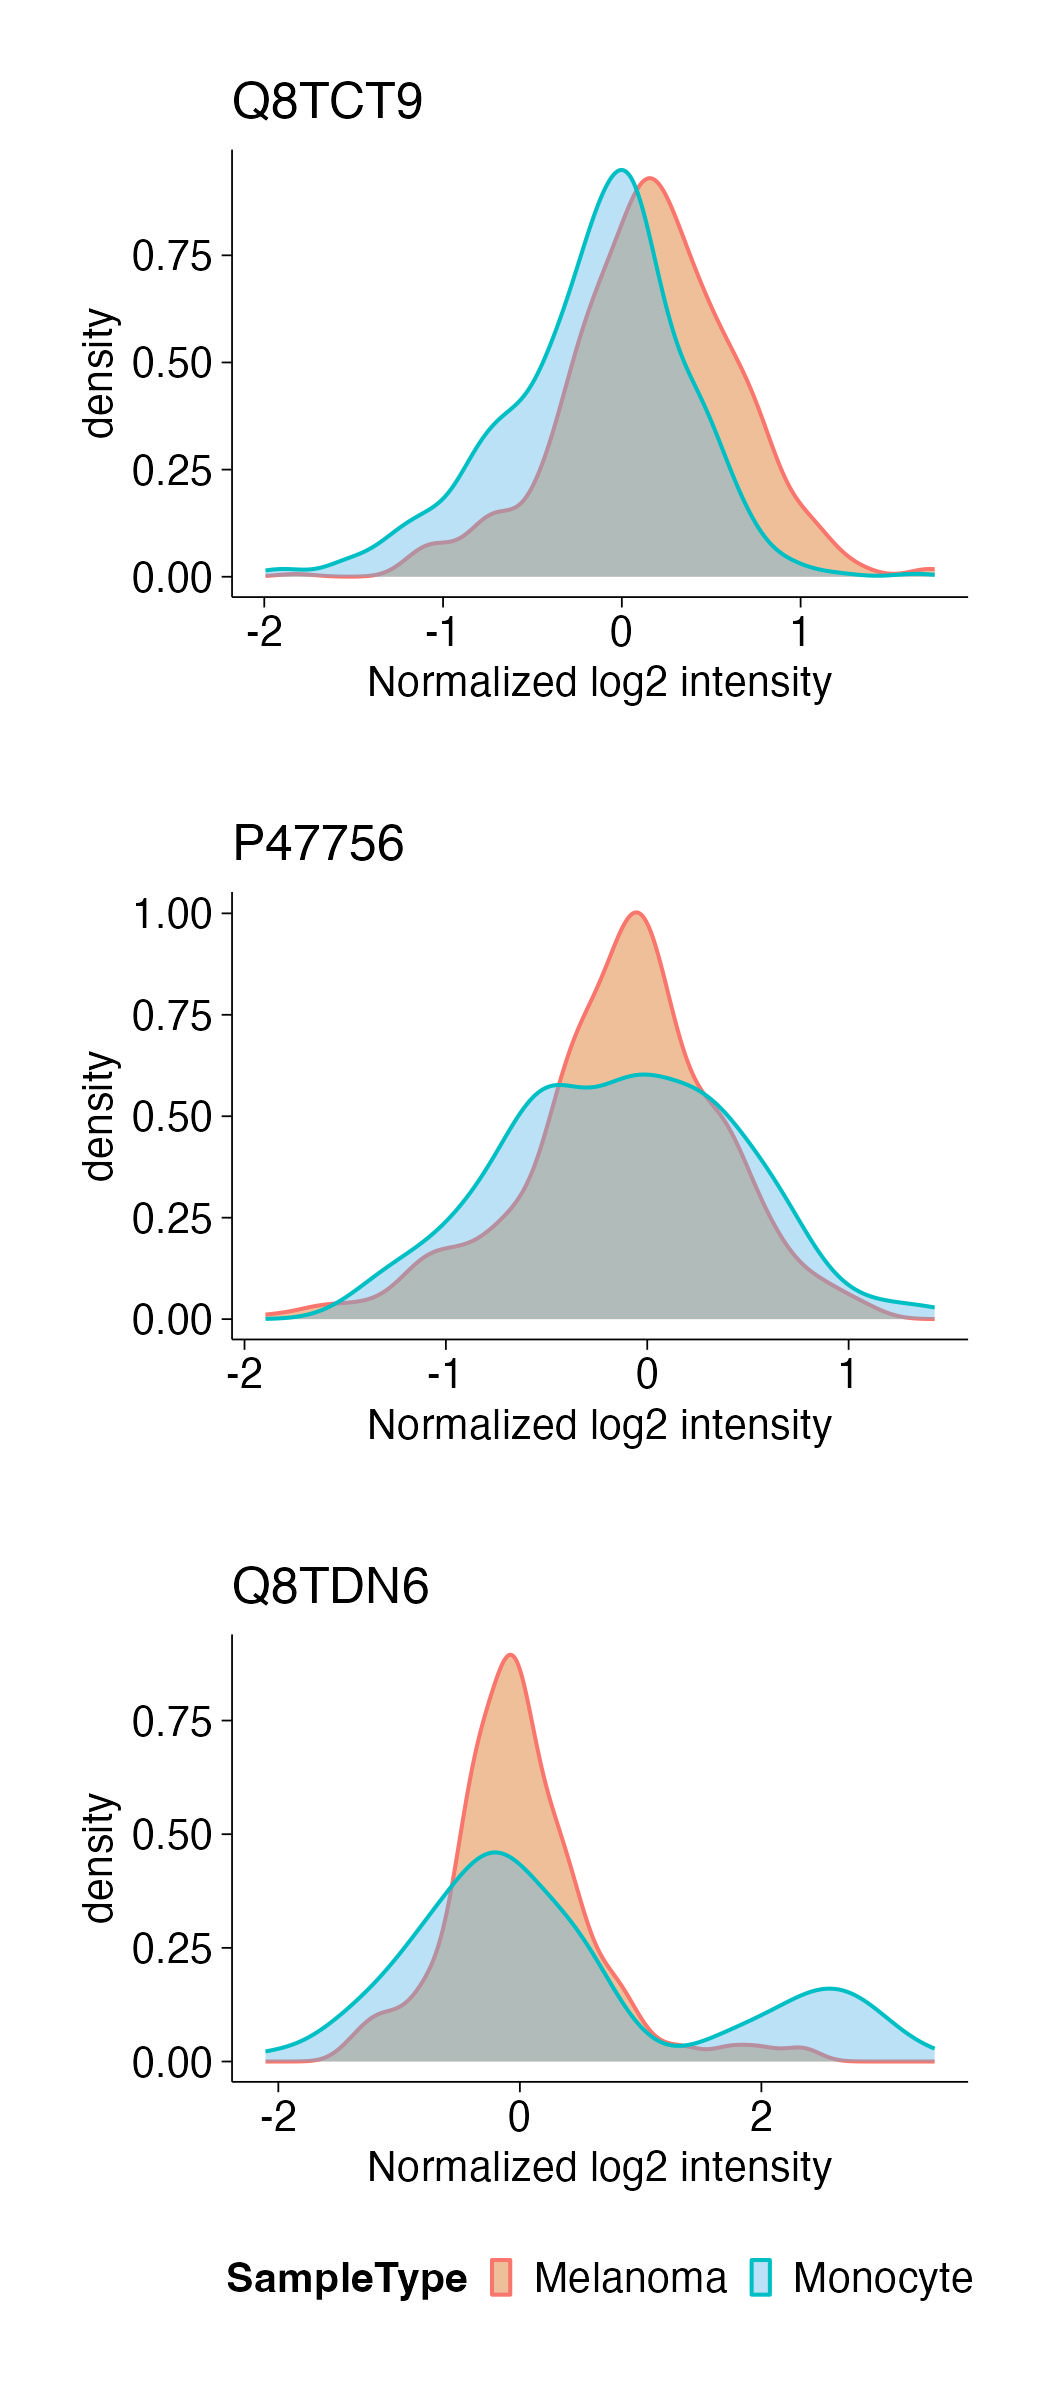
\includegraphics[width=\linewidth]{figs/fig1.jpg}
    \caption{\textbf{Motivating examples of distributional heterogeneity in single-cell proteomics} Density distributions of three proteins from the Leduc single-cell proteomics dataset, comparing melanoma cells (red) and monocytes (blue). The x-axis shows the normalized log2 protein intensity (log2-transformed, median-centered intensities; see Data in Methods), and the protein accession is given above each panel. The left panel (Q8TCT9) illustrates a conventional mean shift between cell types, which is the type of difference that standard DA methods are designed to detect. The middle panel (P47756) shows a difference in variance (Note that there is also a clear difference in kurtosis). The right panel (Q8TDN6) reveals the emergence of a distinct subpopulation in one cell type, visible as a secondary mode. The latter examples reflect differences in shape rather than mean. These are biologically informative yet systematically missed by conventional differential abundance (DA) approaches. They motivate the need for differential distribution (DD) methods capable of detecting the full spectrum of distributional differences in single-cell data.
}
    \label{fig:examples}
\end{figure}

Conventional DA analysis methods are designed to pick up mean shifts, as seen in the left panel in Figure \ref{fig:examples}, but lack power to prioritize proteins for which the distribution between cell populations mainly differs in shape, as seen in the middle and right panels in Figure \ref{fig:examples}.
%This illustrates a fundamental limitation of mean-based approaches: whether or not a distributional difference is deemed significant depends entirely on its impact on the mean.
These changes in shape may reflect underlying biological processes that remain undetected with conventional DA methods. For example, the increased
spread of the abundance values observed in the middle panel may indicate a heterogeneous cellular response, whereas the pattern in the right panel may reflect the emergence of a novel cell state in a subset of cells.
To infer such nuanced but relevant effects, more flexible approaches are required, which are referred to as differential distribution (DD) methods.
\\
\\
Several approaches to perform such DD analysis on single cell data already exist, most notably \texttt{BASiCS} \cite{basics}, \texttt{scDD} \cite{scdd} and \texttt{distinct} \cite{distinct}. However, these methods were developed specifically for single-cell RNA-seq data and have been neither tested on nor tailored for proteomics applications. Moreover, they cannot handle large proportions of missing values, a key problem in SCP datasets, and lack interpretability on how the distributions differ. The latter greatly limits the utility of the assessment, as the nature of the difference is an important element in hypothesizing about the possible causes.\\
Additionally, each approach has methodological limitations: \texttt{BASiCS} is restricted to testing for differences in mean and variance, \texttt{scDD} can only handle count data, and \texttt{distinct} can only be used for two-group comparisons.

Therefore we here present \texttt{gamdid}: a novel statistical framework for DD analysis. \texttt{gamdid} is capable of detecting any form of distributional difference between experimental conditions and provides an interpretable visualization of these effects. Importantly, \texttt{gamdid} also allows users to localize and visualize the specific regions that are differentially distributed, providing a direct link between statistical inference and visualization.\\
By building on the flexible framework of generalized additive models (GAMs), \texttt{gamdid} thus extends well beyond traditional mean-based comparisons while remaining intuitive and highly interpretable.




\section{Results} \label{results}

In this section, we first describe the statistical model and inference procedure underlying \texttt{gamdid}. We then evaluate \texttt{gamdid} through a simulation study and a case study, both based on real SCP data. The simulation study benchmarks \texttt{gamdid} across five distributional scenarios. Subsequently, we demonstrate the practical utility of \texttt{gamdid} through a controlled spike-in case study.

\subsection{Statistical model and inference}
A key advantage of SCP analysis over bulk proteomics is its capacity to assess single-cell heterogeneity. This can result in differences in abundance distributions that are more subtle than mean abundance differences, and are thus overlooked by traditional, bulk-oriented differential analysis methods for proteomics data.\\
Instead of modeling the abundance data with a normal distribution, we here adopt a flexible non-parametric approach to estimate the distribution of the protein abundances in single cells in each group by building upon Lindsey's method \cite{lindsay_method}. Specifically, for each feature the density estimation problem is recast into Poisson regression by discretizing the sample space into bins. In other words, we convert the intensities into histogram bin data, see Figure \ref{fig:workflow} panel A, and the bin counts are then considered independent Poisson-distributed observations.

\begin{figure}[H]
    \centering
    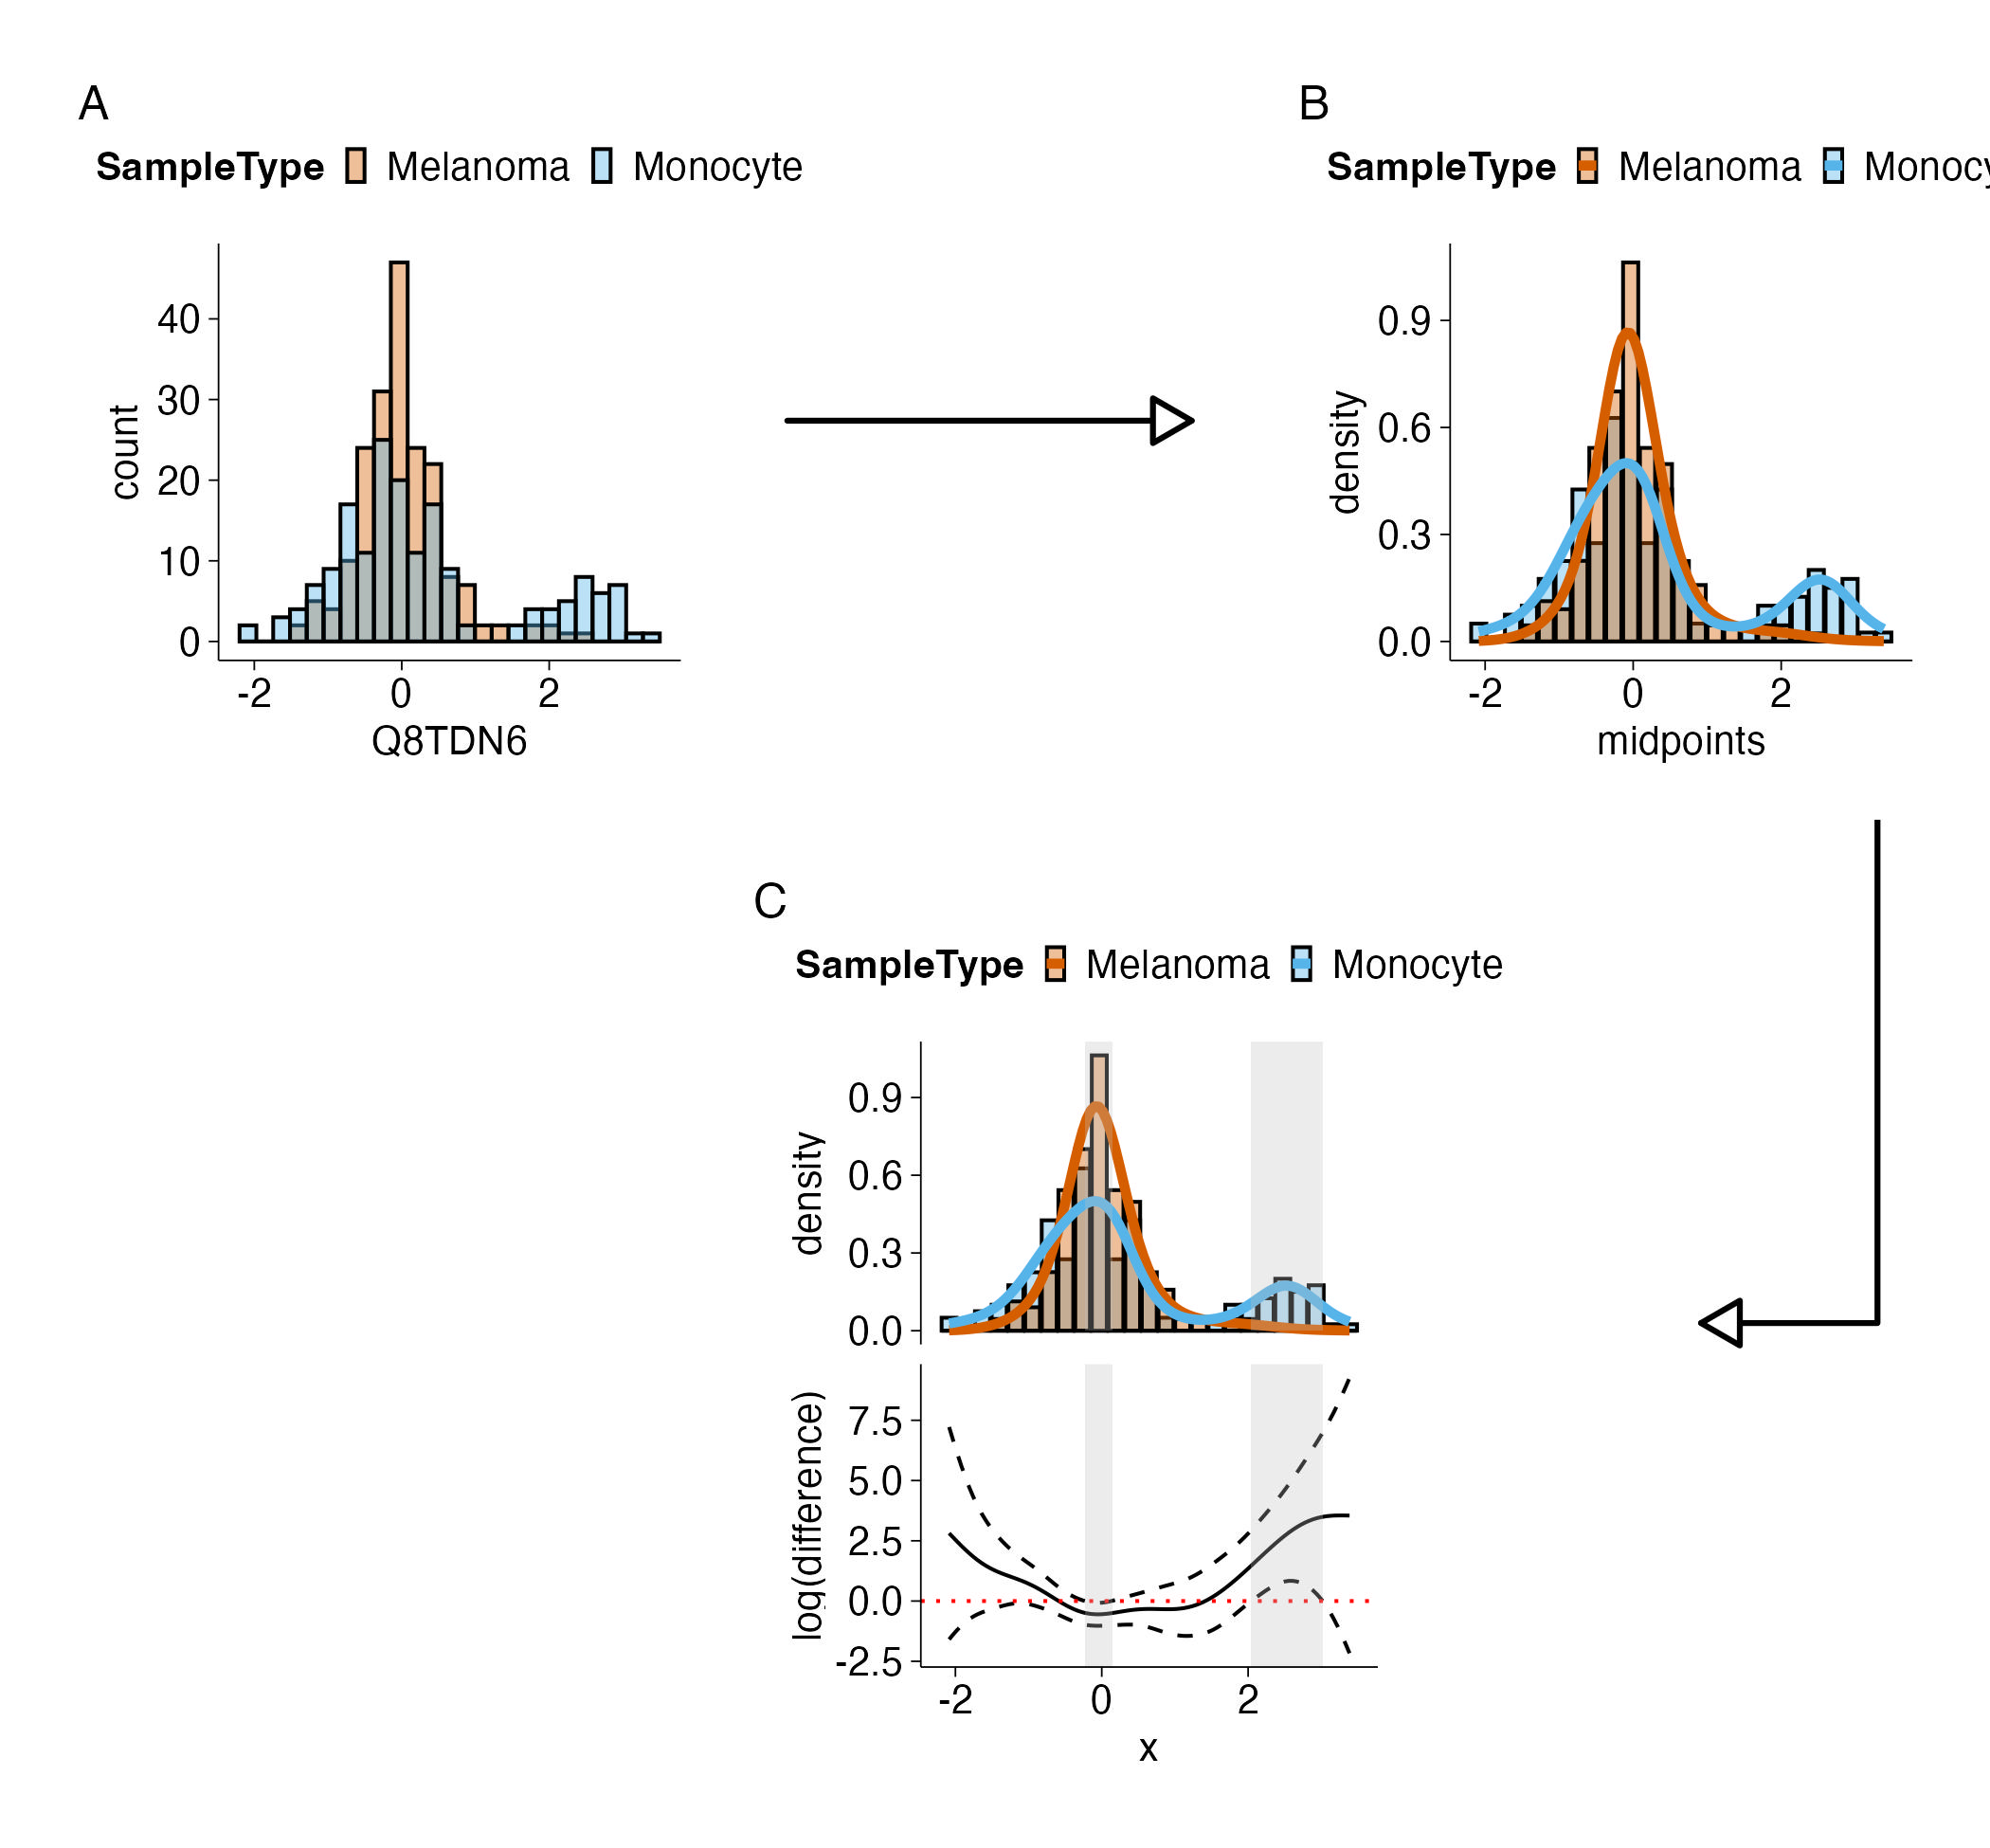
\includegraphics[width=0.85\linewidth]{figs/fig2.jpg}
    \caption{\textbf{Overview of the gamdid workflow} The complete workflow for fitting GAMs to compare distributions is illustrated using a ribosome biogenesis protein from the Leduc dataset. \textbf{A}: Raw protein abundance values are discretized into histogram bin counts, recasting the density estimation problem as Poisson regression. This representation preserves distributional shape information that is lost in a mean-based summary. \textbf{B}: A Poisson generalized additive model (GAM) is fitted to the bin counts as a function of bin midpoints, allowing each group (melanoma and monocyte) to have its own flexible, non-parametric density curve. The GAM framework accommodates any distributional shape without parametric assumptions. \textbf{C} (top): The fitted density curves generated by gamdid's visFit function, with gray shading highlighting regions where the distributions differ significantly between groups. \textbf{C} (bottom): The difference smoother representing the log-ratio of densities between groups along with its simultaneous confidence band. Regions where this band excludes zero identify statistically significant local distributional differences, linking inference to an interpretable visualization. This combination of flexible modeling, hypothesis testing, and interpretable visualization is an innovative feature unique to gamdid.}
    \label{fig:workflow}
\end{figure}

This representation allows for density estimation through Poisson generalized additive models, where expected counts are modeled as a function of the bin midpoints and by specifying a group-specific spline, each group has its own unique density shape. The GAM fits are displayed in Figure \ref{fig:workflow} panel B.

Inference is subsequently carried out using the GAM framework, with differences between groups assessed using Wald-type tests by comparing group-specific model parameters. This yields a p-value for inferring any type of distributional difference both in location and in shape, referred to as the GAM p-value in the remainder of the manuscript.\\
To increase the power to detect distributional changes that are strongly driven by differences in the mean, the p-value obtained from the GAM is combined with a p-value derived from the \texttt{msqrob2} framework, a conventional mean-based approach for DA analysis \cite{msqrob}. The two p-values are integrated using the harmonic mean p-value (HMP) method \cite{harmonicp}.
This results in a final aggregated p-value for each feature, providing a single, robust measure of evidence for any distributional change.

Interestingly, \texttt{gamdid} also provides an interpretable visualization that is directly linked to the inference, by constructing a difference smoother along with a simultaneous confidence band. Regions where this band does not include zero indicate a statistically significant local distributional difference, as illustrated in Figure \ref{fig:workflow} panel C.
%Note However that pinpointing differential regions in the distribution is not possible for all features, sometimes no specific region is significant enough to fall out of the confidence band.
\subsection{Simulation study for benchmarking}
To benchmark \texttt{gamdid} for single cell proteomics applications, we constructed semi-synthetic simulations based on two publicly available mass spectrometry (MS)-based SCP data sets obtained from the R/Bioconductor package \texttt{scpdata} \cite{scp_paper}: the TMT-labeled single-cell Leduc dataset \cite{leduc} consisting of 1531 cells and 6706 identified peptides, and the label-free single-cell Petrosius dataset \cite{petro} consisting of 564 cells and 5729 identified peptides.\\
For each dataset, preprocessed (see Methods) protein-level summarized assays from one cell type were selected and the corresponding cells were randomly assigned to two mock groups (A and B). Hence, all proteins are non-DD between A and B.\\
Only proteins with at least 50 non-missing observations per group were retained for benchmarking, consistent with the default setting in the \texttt{gamdid} package. This threshold ensures a sufficient number of observations to reliably characterize the distribution of each feature, as fewer observations may yield an incomplete or misleading representation of the underlying density.
\\
\\
\textbf{Simulation of distributional differences}
Following the framework established by Korthauer et al. (2016) \cite{scdd}, we introduced five categories of distributional differences by altering protein abundances in cells of group B: differential expression (DE) (a pure mean shift, which corresponds to DA), differential variability (DV), \textcolor{red}{differential both in modality and component means} (DB), differential modality (DM), and differential proportion (DP), as illustrated in Figure \ref{fig:diffsim}. These effects were introduced in 20\% of randomly selected features by systematic shifting of the abundances in subsets of the cells in group B (for the DE, DB, DM and DP scenarios) or by adding controlled random noise (for the DV scenario).

\begin{figure}[H]
    \centering
    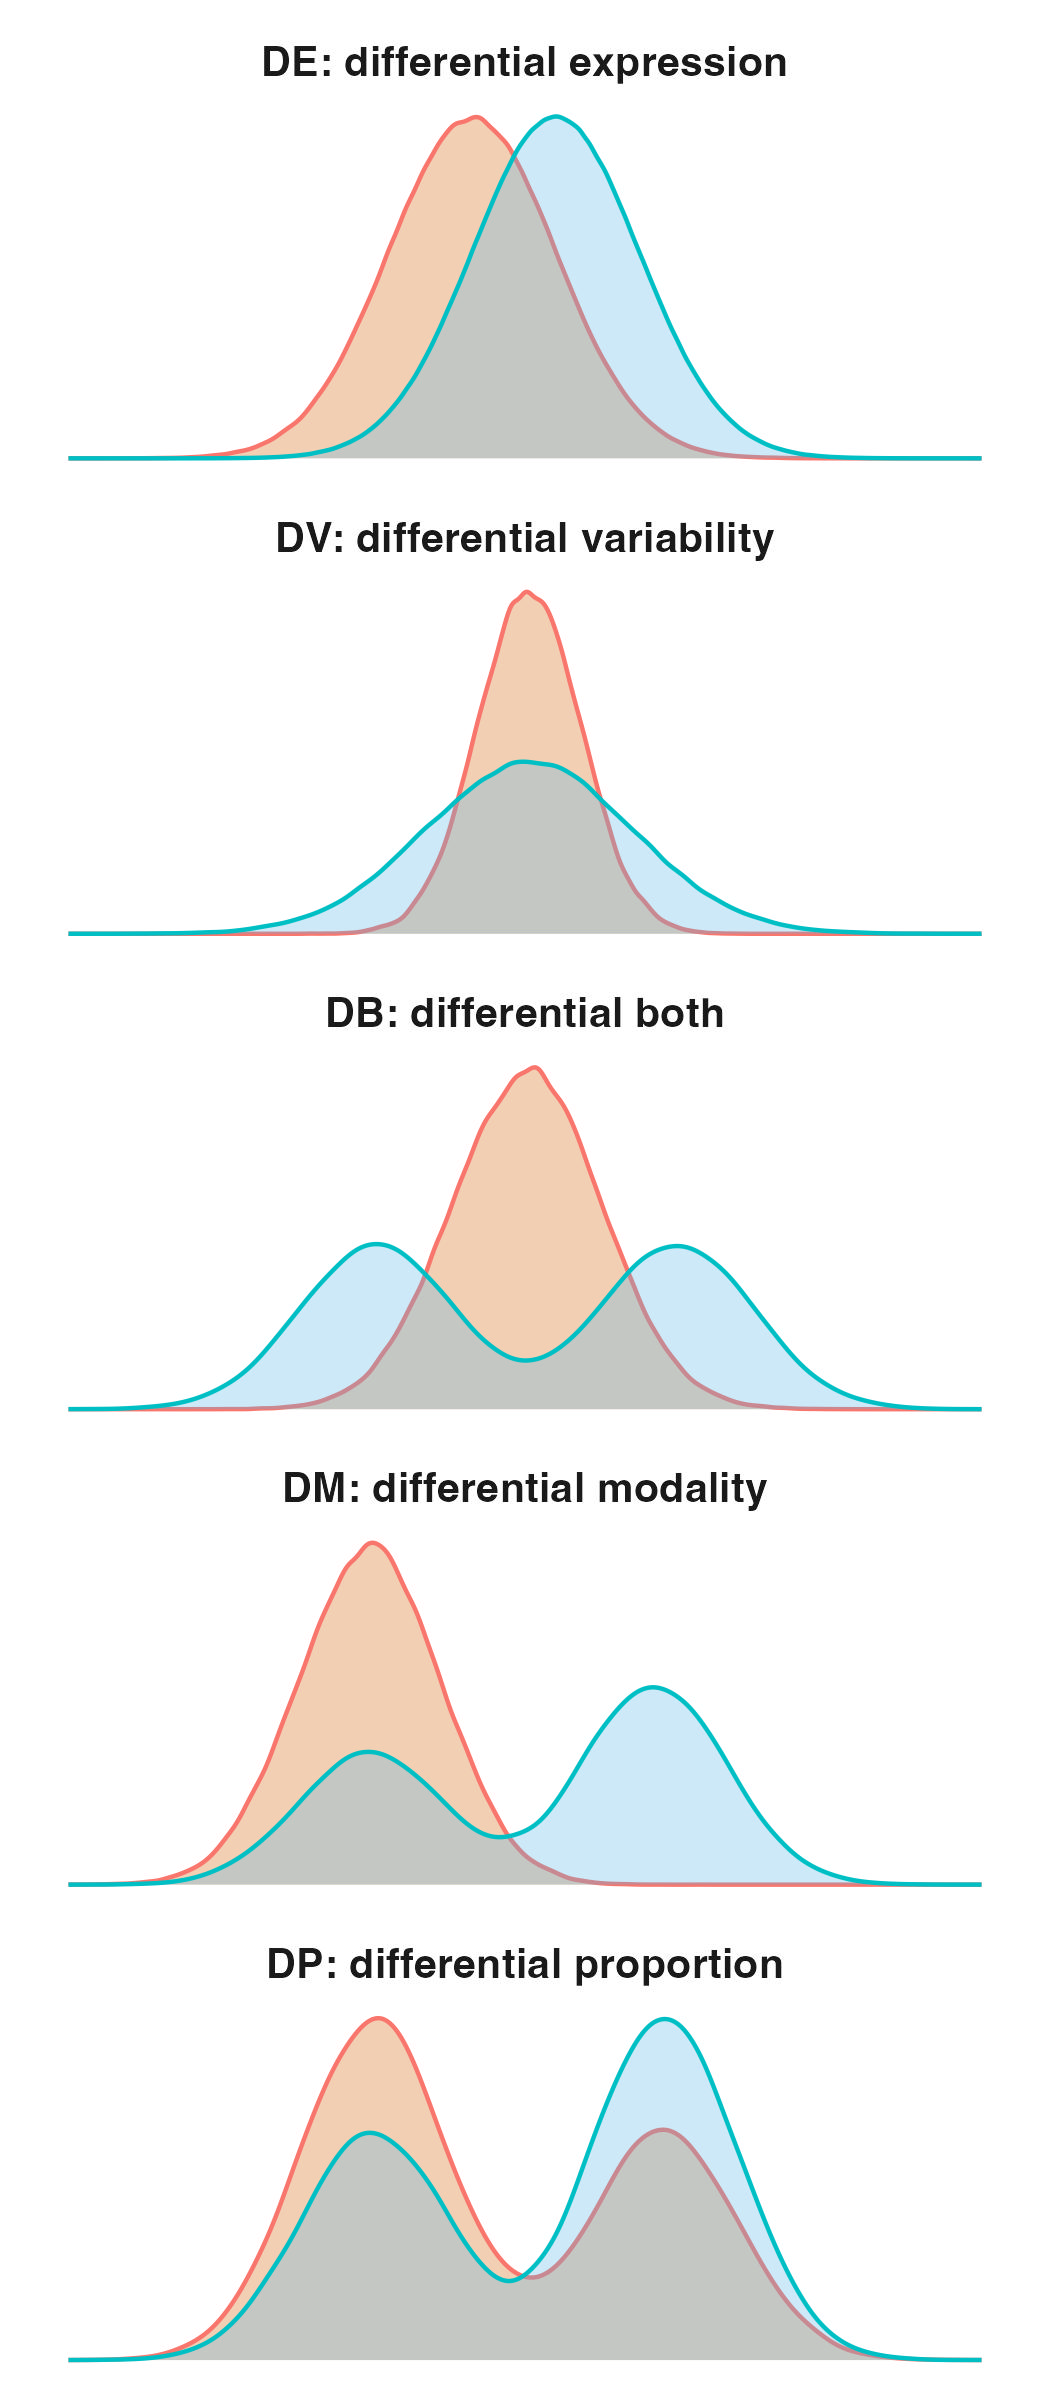
\includegraphics[width=0.425\linewidth]{figs/fig3.jpg}
    \caption{\textbf{Five simulation scenarios used to benchmark gamdid} To evaluate gamdid's ability to detect different types of distributional differences, five categories of signal, established by Korthauer et al. (2016) \cite{scdd}, were introduced into real single-cell proteomics data. \textcolor{red}{DE:} a pure shift in the mean, equivalent to conventional DA. \textcolor{red}{DV:} an increase in variance without a location shift, reflecting e.g. heterogeneous cellular responses. \textcolor{red}{DB:} a bimodal distribution induced in one group by shifting subsets of cells in opposite directions, without altering the overall mean. \textcolor{red}{DM:} an asymmetric shift in one tail, creating a difference in skewness or the emergence of a subpopulation. \textcolor{red}{DP:} a change in the relative weight of a subpopulation shared between groups.}
    \label{fig:diffsim}
\end{figure}

This semi-synthetic approach leverages real SCP data rather than fully synthetic 'clean' simulations, and thus preserves realistic distributional characteristics inherent to single-cell proteomics measurements.
\\
\\
\textbf{Method comparison}
We compare \texttt{gamdid} to \texttt{distinct} as the primary benchmark method. \texttt{BASiCS} and \texttt{scDD} were excluded from the comparison as \texttt{BASiCS} is limited to detecting shifts in mean and variance, and therefore cannot be applied to the majority of the simulations, while \texttt{scDD} requires count data as input, which is incompatible with the continuous abundance measurements obtained in proteomics data.

\texttt{distinct} performs group comparisons by computing the average difference between empirical cumulative distribution functions (ECDFs) and can optionally account for subgroup structure in multi-sample multi-cell designs. As our datasets, similar to most public SCP datasets, do not have these multi-sample multi-cell designs, \texttt{distinct} was applied without this option.\\
Note that the current implementation of \texttt{gamdid} does not account for subgroup structure.\\
Method performance is evaluated using false discovery proportion — true positive proportion (FDP-TPP) curves. For a given significance threshold, the FDP represents the proportion of false positives among all features called significant, while the TPP represents the proportion of true positives recovered out of all truly differential features. An FDP-TPP curve allows one to assess the power of a method (TPP) at any given level of false discoveries (FDP). This provides a more complete picture of method performance than a single summary statistic, and allows for a direct visual comparison of the trade-off between sensitivity and false discovery control across competing methods. A method can be considered more powerful when the area under its FDP-TPP curve is larger. The dashed vertical line at FDP = 0.05 serves as a reference for the nominal FDR threshold.
\\
\\
\textbf{GAM evaluation}
We first evaluate the performance of the GAM methodology in isolation (without p-value aggregation via \texttt{msqrob2}) against \texttt{distinct}. \textcolor{red}{The FDP-TPP curves for both datasets are presented in Figure \ref{fig:leducsims_gam}.}

The GAM method demonstrates conservative false discovery rate control and exhibits substantially superior performance compared to \texttt{distinct} when distributional changes do not involve shifts in mean (DV and DB scenarios). Conversely, in the scenarios where mean shifts contribute to the distributional change, \texttt{distinct} outperforms the GAM method and is even on par with conventional DA analyses like \texttt{msqrob2}. This observation motivated the aggregation of GAM-derived p-values with \texttt{msqrob2} p-values, thereby combining the GAM methodology's sensitivity to differences in shape with \texttt{msqrob2}'s established performance for detecting mean shifts.

\begin{figure}[H]
    \centering
    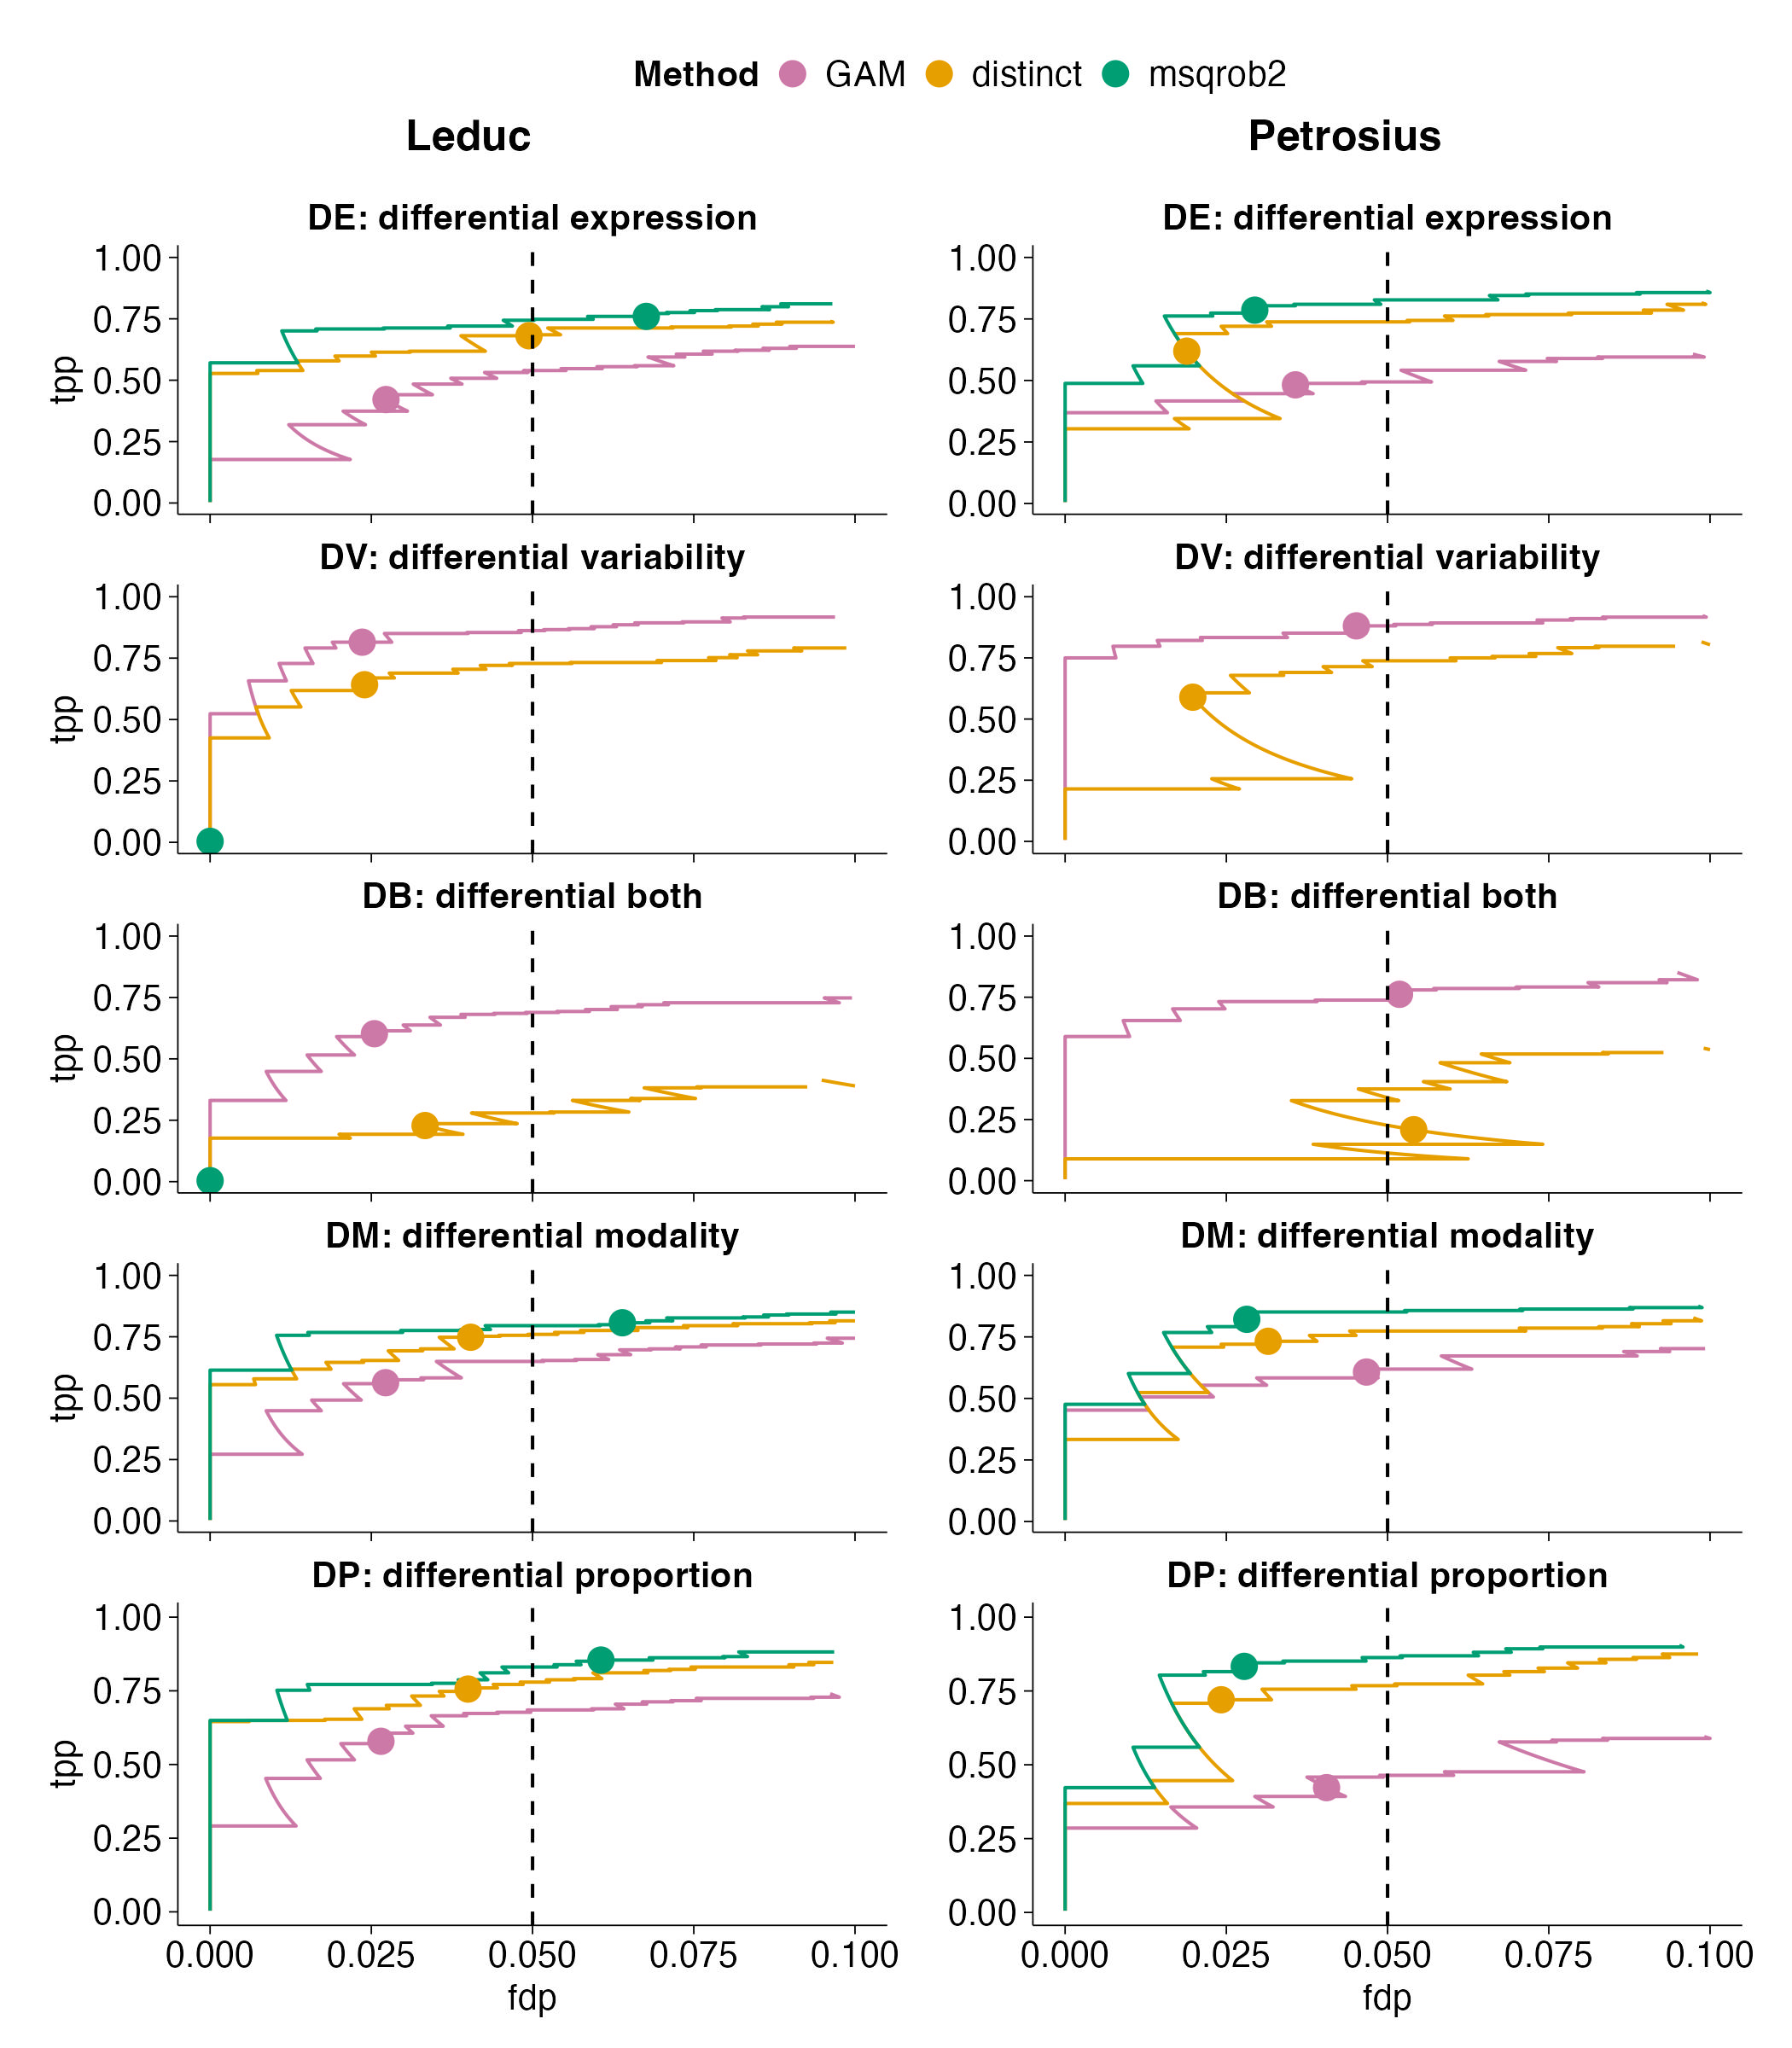
\includegraphics[width=0.85\linewidth]{figs/fig4.jpg}
    \captionsetup{labelfont={bf,small,color=red}}
    \caption{\textbf{\textcolor{red}{Performance of the standalone GAM method}} FDP-TPP curves comparing the standalone GAM method, msqrob2, and distinct across the five simulation scenarios, based on the protein-level mock data of the Leduc dataset (left; 755 monocytes) and the Petrosius dataset (right; 269 m2i cells). Each curve traces the trade-off between TPP (sensitivity) and FDP as the significance threshold is varied; the dots mark the 5\% FDR threshold and the dashed vertical line marks FDP = 0.05. The GAM method achieves conservative FDR control. For distributional changes that do not involve a mean shift (DV, DB), the GAM method substantially outperforms distinct in both datasets, demonstrating its superior sensitivity to shape differences. However, for scenarios where mean shifts contribute to the distributional change (DE, DM, DP), distinct and msqrob2 outperform the standalone GAM method. This complementarity motivates the aggregation of GAM p-values with msqrob2 p-values in the gamdid pipeline. Notably, improvements of the GAM method over distinct are more pronounced in the Petrosius dataset,
which is attributable to the smaller sample size: contrary to gamdid, distinct relies on permutation-based inference and suffers from
reduced null distribution resolution with fewer observations. DB (differential both) denotes a difference in both modality and component means.}
    \label{fig:leducsims_gam}
\end{figure}


\textbf{gamdid evaluation}
Figure \ref{fig:leducsims_gamdid} presents the FDP-TPP curves comparing \texttt{distinct} and \texttt{gamdid} for both datasets. The corresponding numbers of true and false positives at the 5\% FDR threshold are also provided in the supplementary materials (Figures \ref{fig:TP} and \ref{fig:FP}): \texttt{gamdid} recovers a comparable or larger number of true positives, while the false positives are similarly low for both methods.
\texttt{gamdid}'s performance is comparable to \texttt{distinct} for pure mean shifts (DE), shows modest improvements for distributional changes that involve location shifts (DM, DP), and shows substantial improvements for distributional changes in shape (DV, DB).

Improvements are more pronounced in the Petrosius simulations, which could be attributable to the smaller sample size in the Petrosius dataset compared to Leduc.
To examine this, we subsampled the Leduc dataset such that the average number of non-missing observations per group over all features matched that of the Petrosius dataset. The resulting FDP-TPP curves are provided in the supplementary materials in Figure \ref{fig:leducsims_gamdid_subsample}. Indeed, the improvements are more pronounced in the subsampled simulations compared to the Leduc simulations in Figure \ref{fig:leducsims_gamdid}. This supports the hypothesis that \texttt{gamdid} exhibits higher power under smaller sample conditions compared to \texttt{distinct}, which suffers from a reduced resolution of the null distribution due to a limited number of permutations.

\begin{figure}[H]
    \centering
    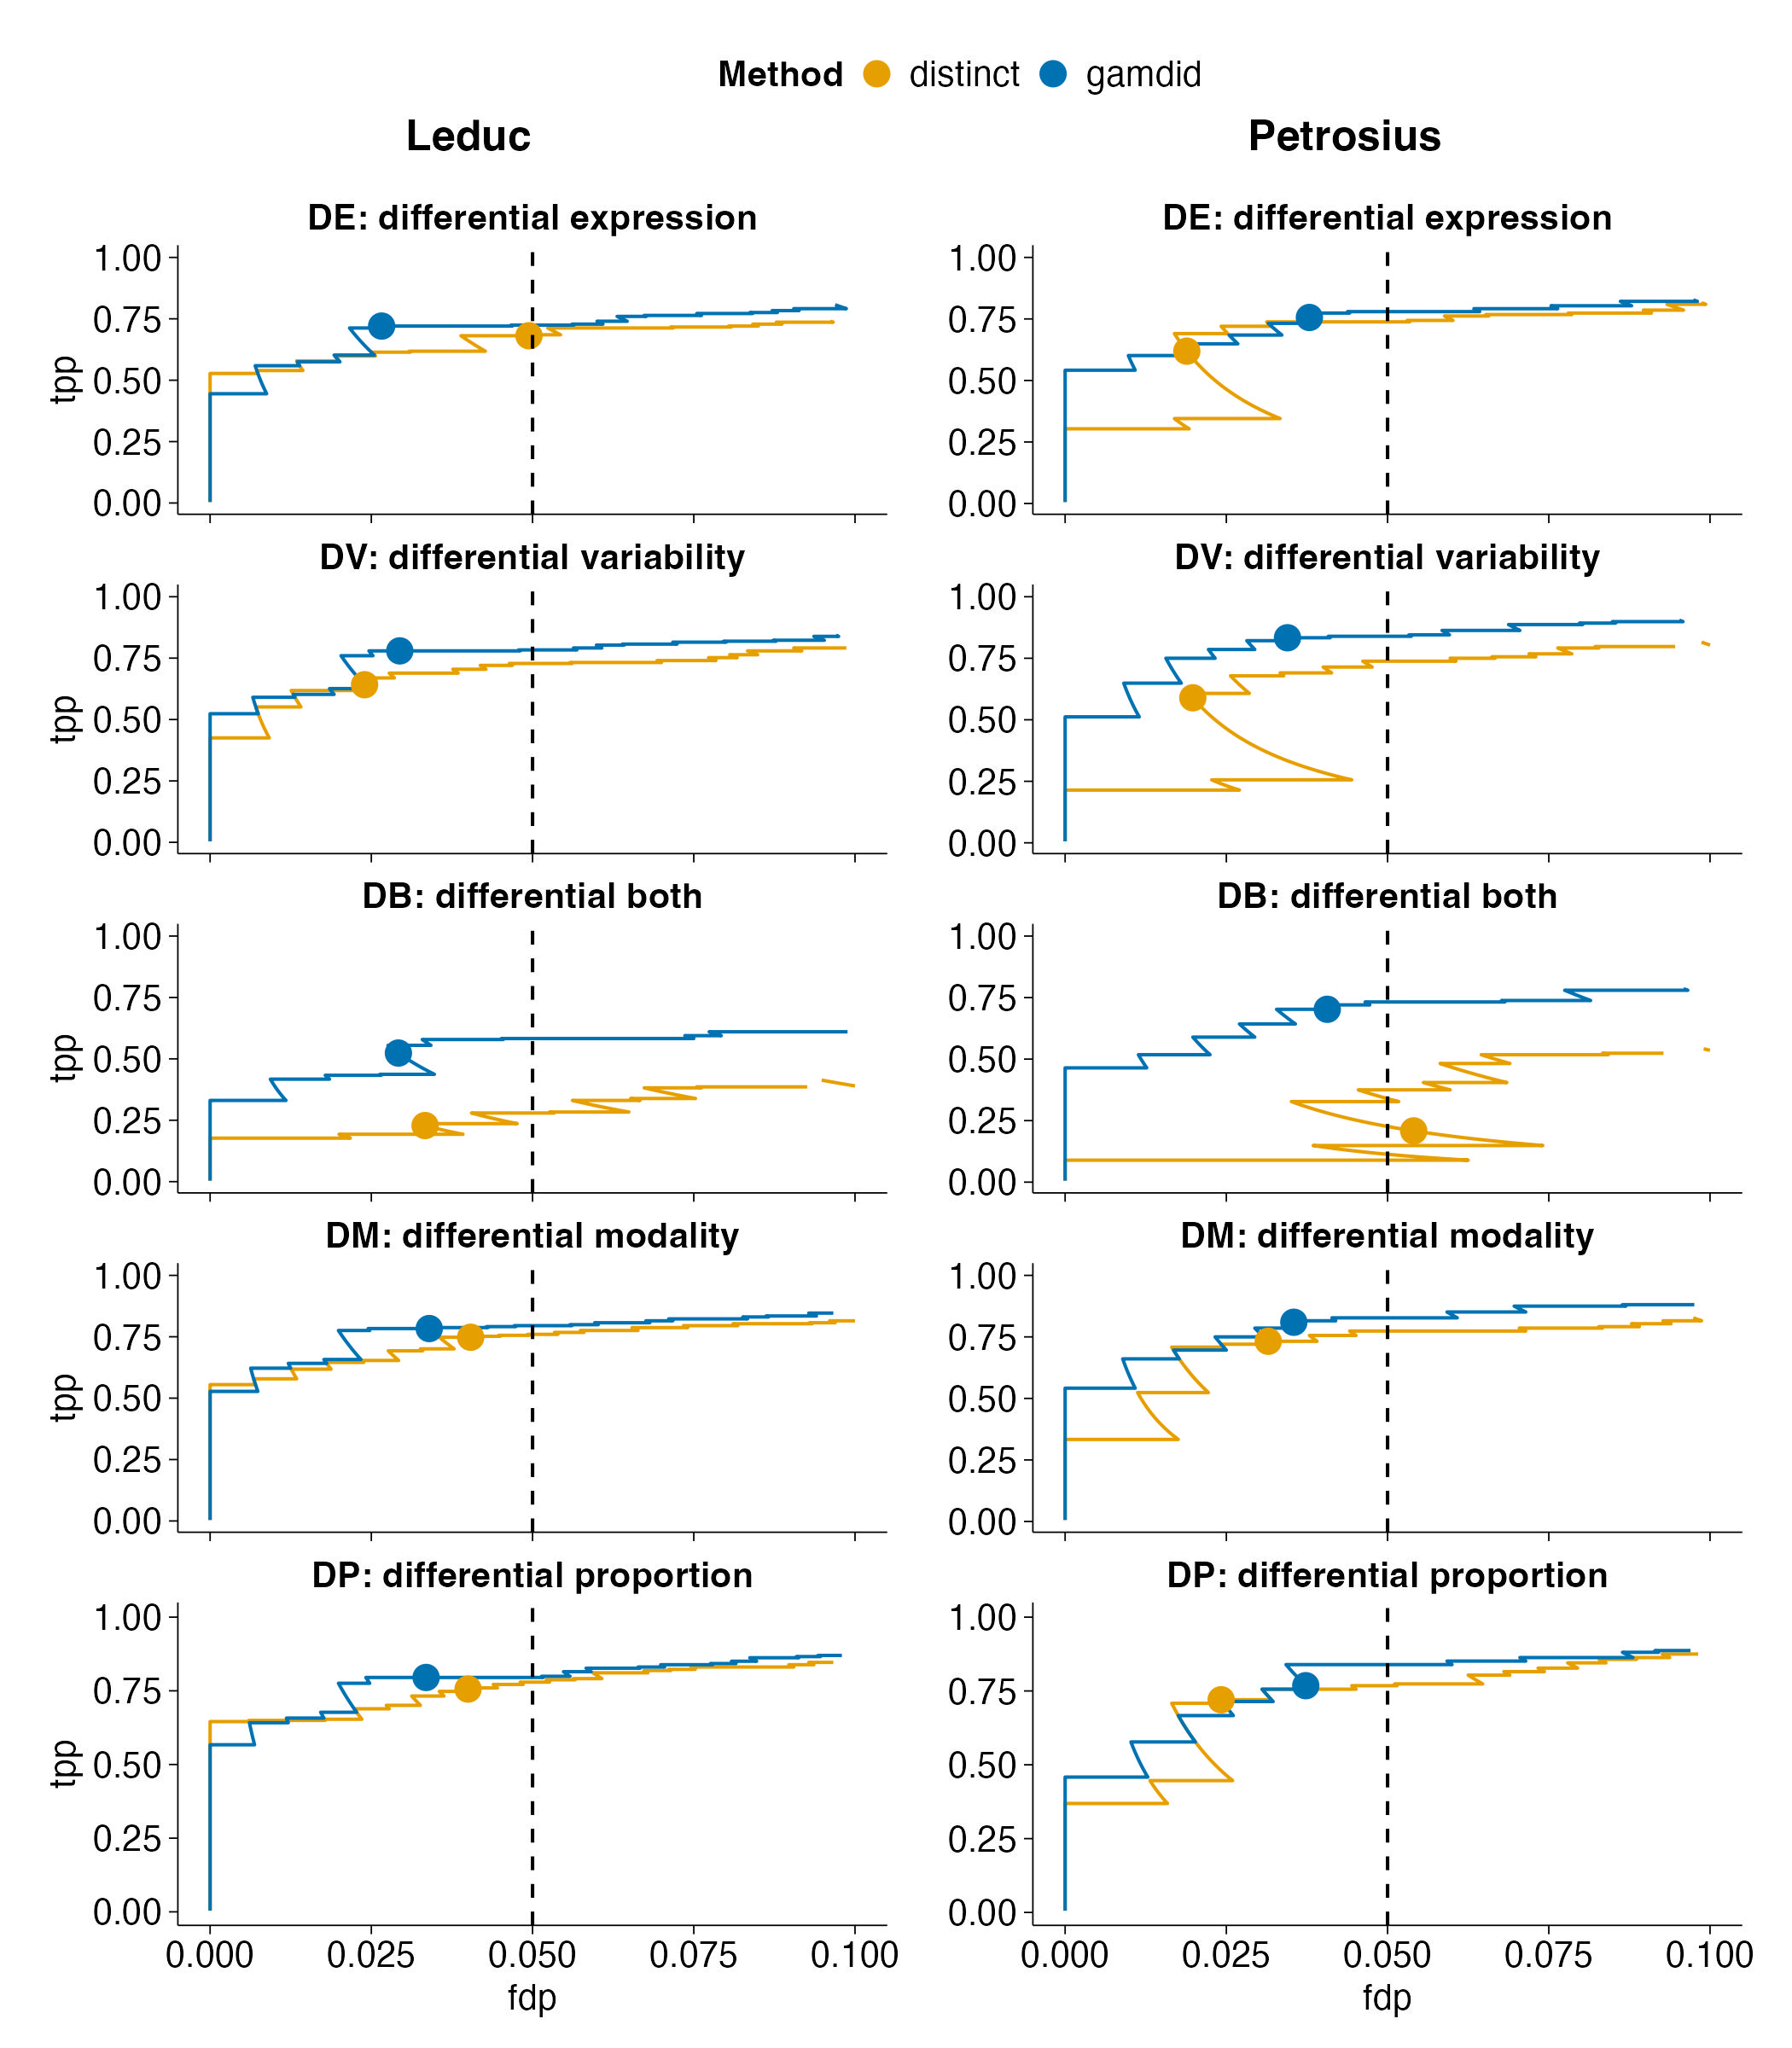
\includegraphics[width=0.85\linewidth]{figs/fig5.jpg}
    \captionsetup{labelfont={bf,small,color=red}}
    \caption{\textbf{\textcolor{red}{Performance of gamdid}} FDP-TPP curves comparing the gamdid method (combining GAM and msqrob2 p-values via the harmonic mean p-value) against distinct across the five simulation scenarios, based on the protein-level mock data of the Leduc dataset (left; 755 monocytes) and the Petrosius dataset (right; 269 m2i cells). The dots mark the 5\% FDR threshold and the dashed vertical line marks FDP = 0.05. By combining the local density sensitivity of the GAM with the established power of msqrob2 for mean shifts, gamdid achieves performance that is comparable to distinct for pure mean shifts (DE), shows modest improvements for distributional changes that involve a location component (DM, DP), and demonstrates substantial improvements for pure shape changes (DV, DB). gamdid maintains conservative FDR control throughout. These results demonstrate that p-value aggregation successfully bridges the complementary strengths of both components, yielding a single method competitive across the full spectrum of distributional differences. DB (differential both) denotes a difference in both modality and component means.}
    \label{fig:leducsims_gamdid}
\end{figure}




To assess the robustness of the conclusions under less pronounced distributional differences, FDP-TPP curves for simulations with 25\% reduced signal magnitudes are provided in the supplementary materials (Figure \ref{fig:leducsims_lower_gamdid}). These results are consistent with the findings above, indicating robust performance.

\textbf{Interpretation and visualization}
In contrast to competing methods, \texttt{gamdid} provides informative visualizations of features picked up as DD. Figure \ref{fig:DV_example} illustrates this functionality for a significant feature identified under the DV simulation framework. This visualization integrates GAM fits with highlighted differential regions, providing immediate visual evidence of differential variability between groups.

\begin{figure}[H]
    \centering
    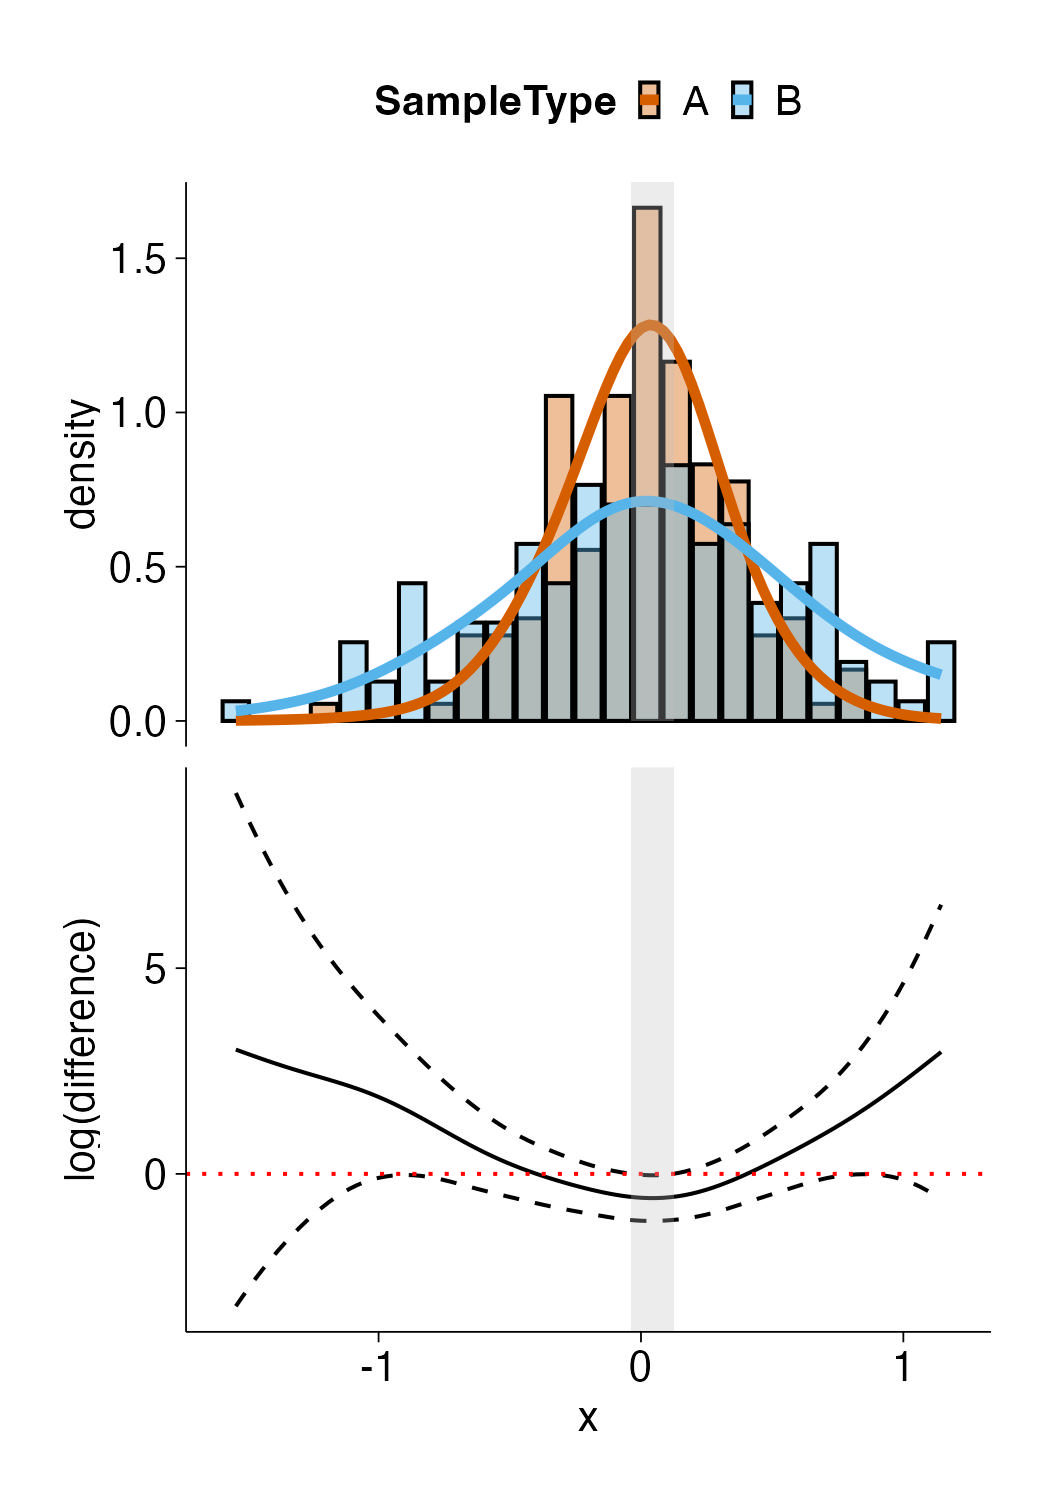
\includegraphics[width=0.425\linewidth]{figs/fig6.jpg}
    \caption{\textbf{gamdid's interpretable visualization for a DV-simulated feature in the Petrosius dataset} A feature with induced differential variability (DV simulation), visualized using gamdid's visFit function. The top panel shows the fitted GAM density curves for both groups, overlaid on the observed histograms. The bottom panel displays the difference smoother (log-ratio of densities) along with its simultaneous confidence band; the gray-shaded region identifies the specific abundance range where the distributional difference is statistically significant. Unlike competing DD methods such as distinct, gamdid does not merely return a p-value; this visualization provides immediate visual evidence of differential variability between groups.}
    \label{fig:DV_example}
\end{figure}


\textbf{Peptide-level simulations}
The same simulation framework was applied to peptide-level assays for both the Leduc and Petrosius datasets. The resulting FDP-TPP curves are provided in the supplementary materials in Figure \ref{fig:leducsims_pep} and are consistent with the protein-level results.\\
Note, however, that the FDR control at the nominal 5\% threshold is less conservative at the peptide level due to the correlation structure inherent to peptide-level data, a well-known challenge in peptide-level analyses. Nevertheless, this demonstrates that \texttt{gamdid} provides a flexible framework suitable for inferring DD at different quantification levels (precursor, peptide, protein) in MS-based proteomics data.
\\
\\
\textbf{Three-group simulations}
A unique advantage of \texttt{gamdid} is its support for omnibus testing across more than two groups, followed by post-hoc pairwise comparisons corrected for multiple testing using the stagewise testing procedure \cite{stagewise_testing}. The omnibus test simultaneously assesses whether any distributional difference exists between any  of the groups. No competing DD analysis method currently offers this functionality.\\
To evaluate this functionality, we extended the simulation framework described above to a three-group setting, randomly assigning cells to mock groups A, B, and C, with distributional signal introduced in group B under the same five simulation scenarios as above. The omnibus test was applied to this three-group comparison and the resulting FDP-TPP curves are provided in the supplementary materials in Figure \ref{fig:leduc_threegroup}. Note that, as none of the competing DD methods supports multi-group testing, a formal benchmark comparison is not possible here.\\
Interestingly, the three-group setting yields higher power than the two-group comparison under equal signal strength. Note that this might arise from the default minimum observation requirement of 50 cells per group imposed by \texttt{gamdid}, which, in the three-group analysis, requires more observations than in the two-group analysis, leading to more powerful inference.
\subsection{Case study}
We next illustrate the utility of \texttt{gamdid} in a case study based on the Leduc dataset.\\
First, we randomly divide the monocyte cells into two mock groups: X (containing 377 cells) and Y (containing 378 cells). In group Y, we spike in 10\% of the 697 sub-cluster A melanoma cells (69 cells) to simulate a subpopulation in group Y.\\
Figure \ref{fig:volanoPlots} shows the volcano plot of the conventional DA \texttt{msqrob2} analysis twice. In panel A, significant features of the DA analysis are marked in red, while in panel B the significant features of DD methods \texttt{gamdid} and \texttt{distinct} are marked.

\begin{figure}[H]
    \centering
    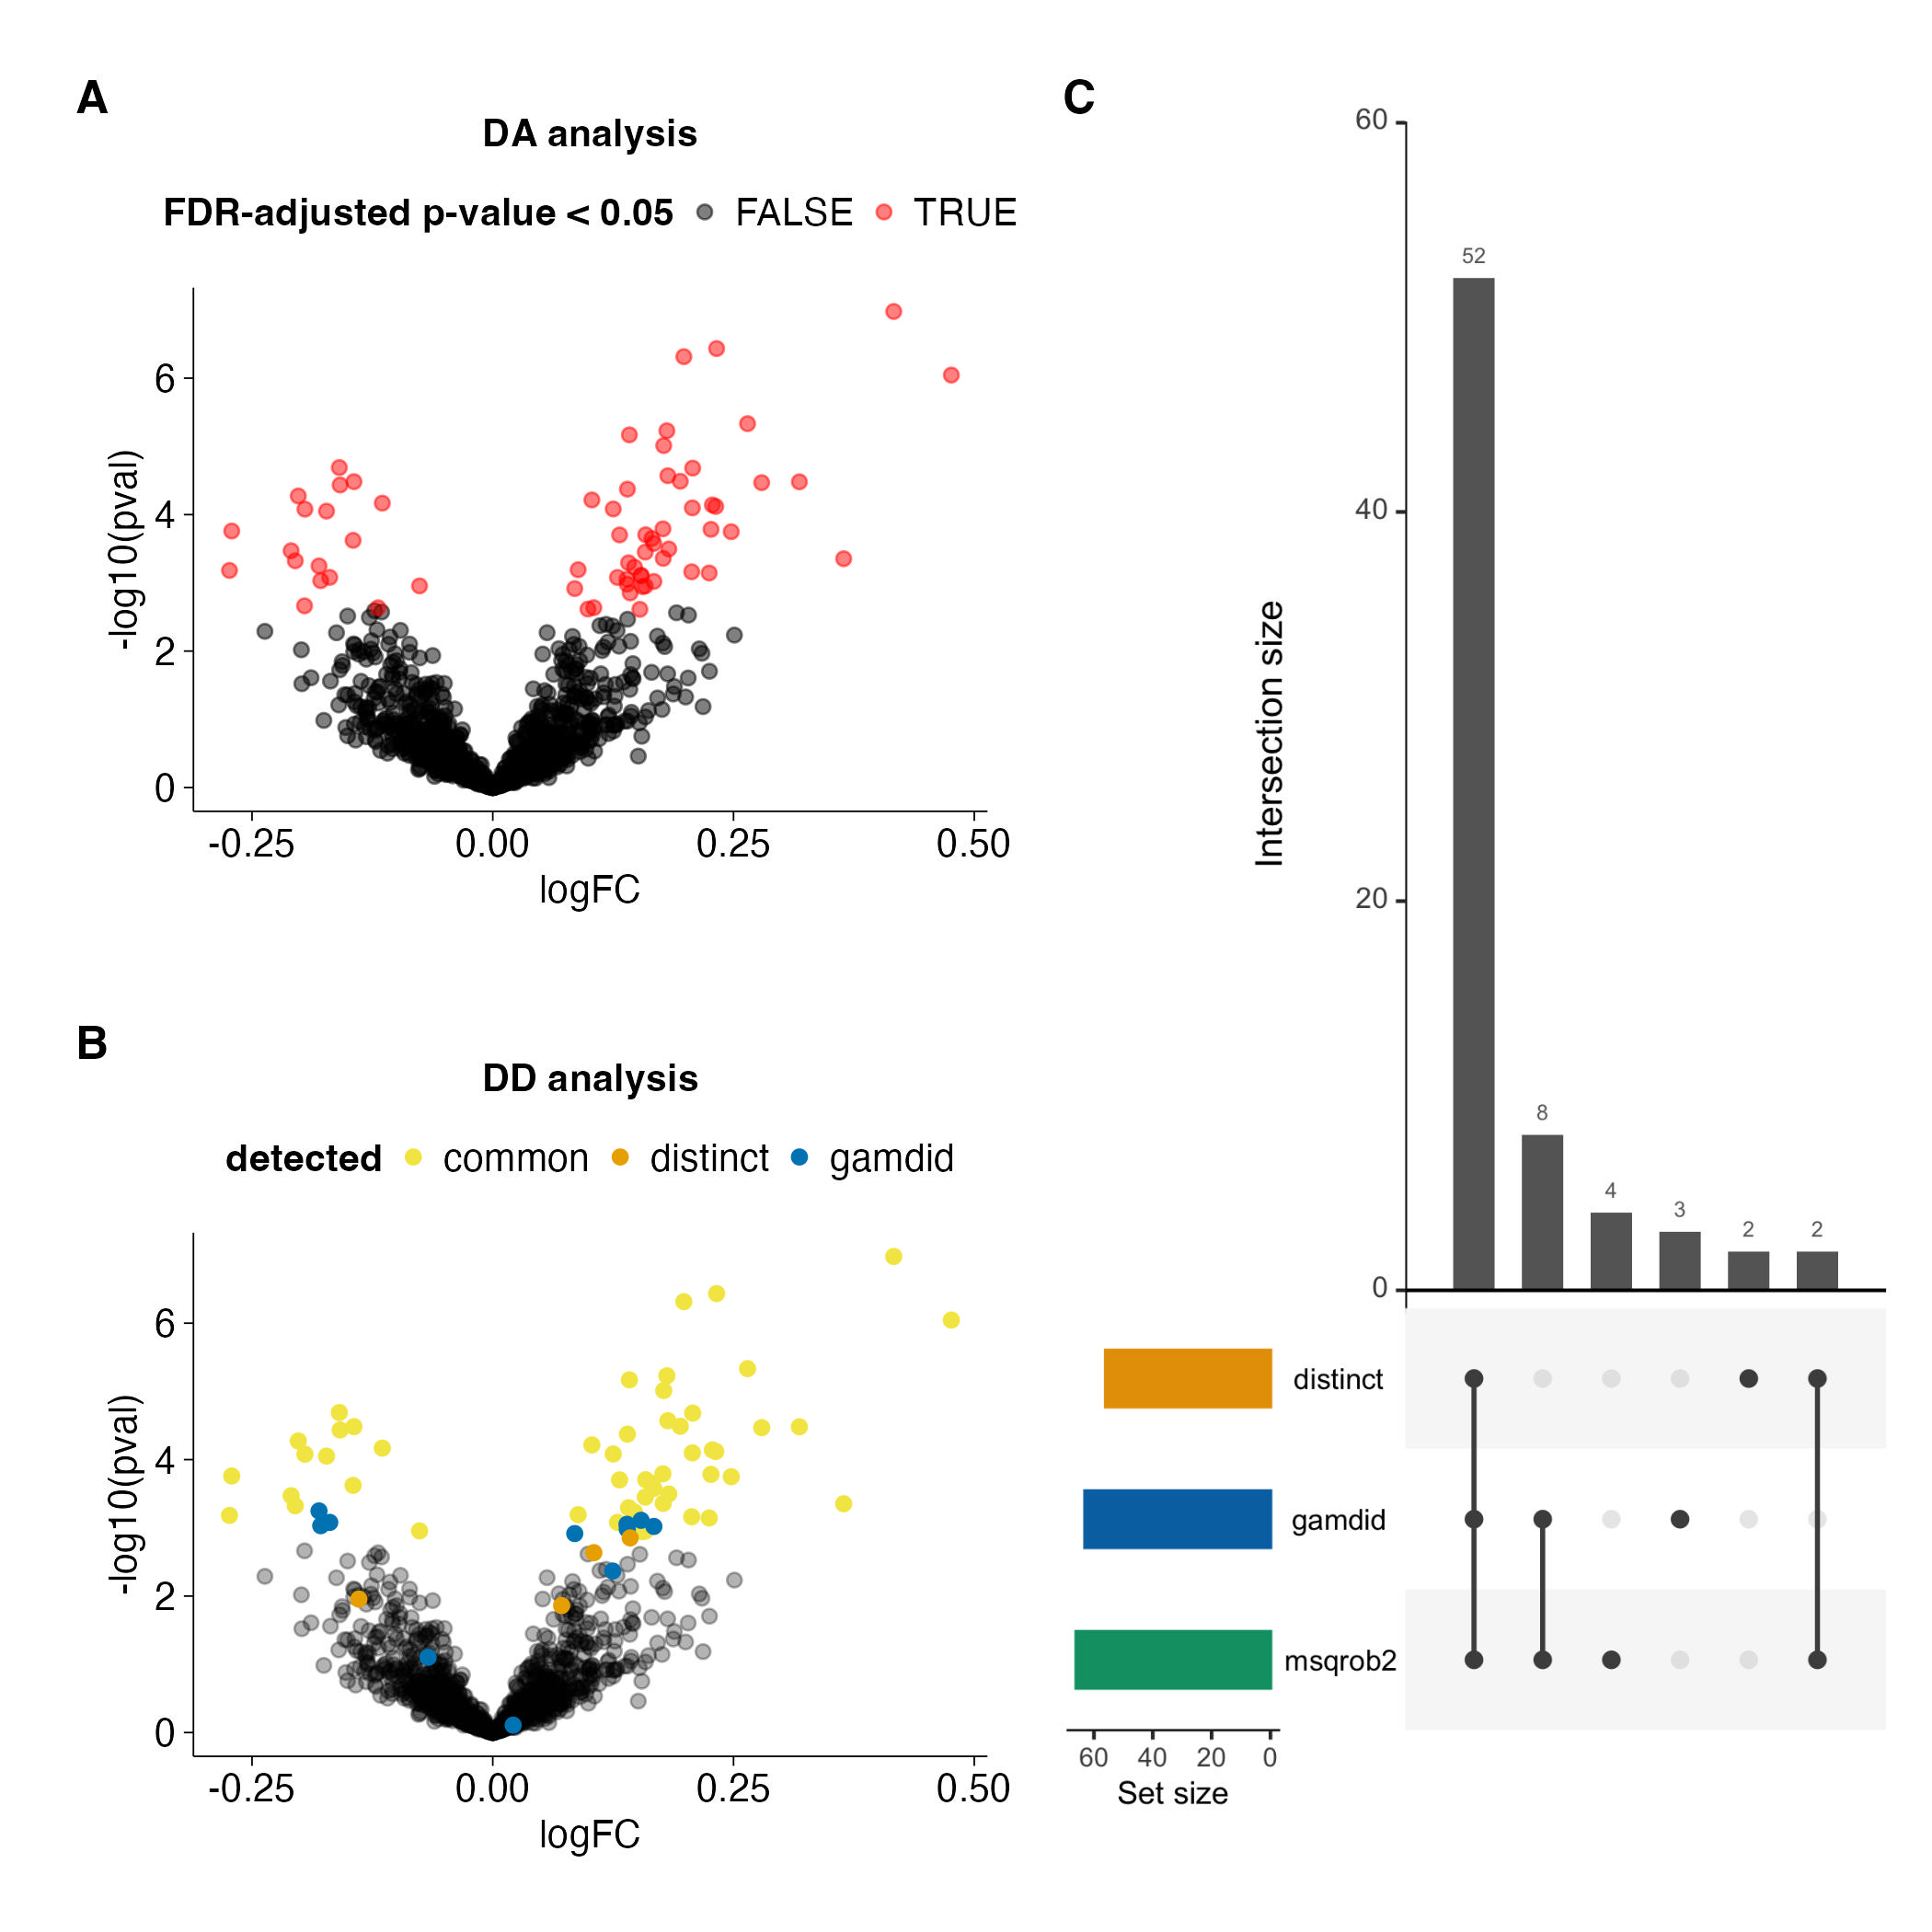
\includegraphics[width=0.85\linewidth]{figs/fig7.jpg}
    \captionsetup{labelfont={bf,small,color=red}}
    \caption{\textbf{\textcolor{red}{Case study: gamdid detects distributional changes missed by conventional DA analysis}} A controlled spike-in experiment based on the Leduc dataset: monocyte cells are split into two mock groups (X: 377 cells; Y: 378 cells), and 10\% of the 697 sub-cluster A melanoma cells (69 cells) are spiked into group Y to simulate the emergence of a subpopulation. Panels A and B display the same msqrob2 volcano plot. \textbf{A}: Features found significant by conventional DA (msqrob2) are highlighted in red. \textbf{B}: The same volcano plot, now colored by DD method detection: yellow = detected by both distinct and gamdid; orange = detected by distinct only; blue = detected by gamdid only. Both DD methods detect the majority of DA features, while also prioritizing some features missed by conventional DA methods. \textbf{C}: UpSet plot showing the overlap in significant features between distinct, gamdid and msqrob2. The horizontal bars (left) show the total number of significant features per method (Set size); the vertical bars (top) show the size of each intersection, with the dot matrix below indicating which methods contribute to each intersection. The six features picked up by msqrob2 and missed by gamdid are borderline significant for msqrob2 and borderline non-significant for gamdid (this is not the case for distinct, see Table \ref{tab:only_msqrob2}), which means that only gamdid largely preserves the ranking of DA features. Moreover, gamdid prioritizes three features that are missed by both msqrob2 and distinct (see Table \ref{tab:only_gamdid}).}
    \label{fig:volanoPlots}
\end{figure}

Figure \ref{fig:volanoPlots}C presents a method comparison for
the significant features in the spike-in case study. Overall, the methods produce
similar results with 52 features found significant by all three.


Only six features are picked up by \texttt{msqrob2} and missed by \texttt{gamdid}.
These features are borderline significant for \texttt{msqrob2} and borderline
non-significant for \texttt{gamdid}, which is illustrated in table
\ref{tab:only_msqrob2} in supplementary materials.\\
Furthermore, \texttt{gamdid} prioritizes three features that \texttt{msqrob2}
and \texttt{distinct} fail to detect (see Table \ref{tab:only_gamdid} in
supplementary materials).
Interestingly, even features detected by all three methods illustrate the utility
of \texttt{gamdid}. Figure \ref{fig:caseStudy_exs} shows the
\texttt{gamdid} visualization for four representative features (panels A--D), displaying the
mock groups (top) and the spike-in study (middle). The boxplot at the bottom of each panel
indicates where the spiked-in melanoma cells are
located within the distribution of group Y. Figure \ref{fig:caseStudy_exs} clearly
shows that these features are DD due to the subpopulation of spike-in cells rather
than DA. Additionally, it powerfully validates gamdid’s localization approach:
not only does gamdid detect the distributional change, it correctly identifies
its location, providing interpretable visualization that is unavailable in any
competing DD method.

% Figure \ref{fig:caseStudy_example} shows the
% \texttt{gamdid} visualization of one of these three features, displaying the
% mock groups (top) and the spike-in study (bottom).

The \texttt{gamdid} visualizations of two of the four features
only detected by \texttt{msqrob2} and of the two features only detected by
\texttt{distinct} are provided in supplementary materials in
Figure \ref{fig:msqrob_distinct_only}.

\begin{figure}[H]
    \centering
    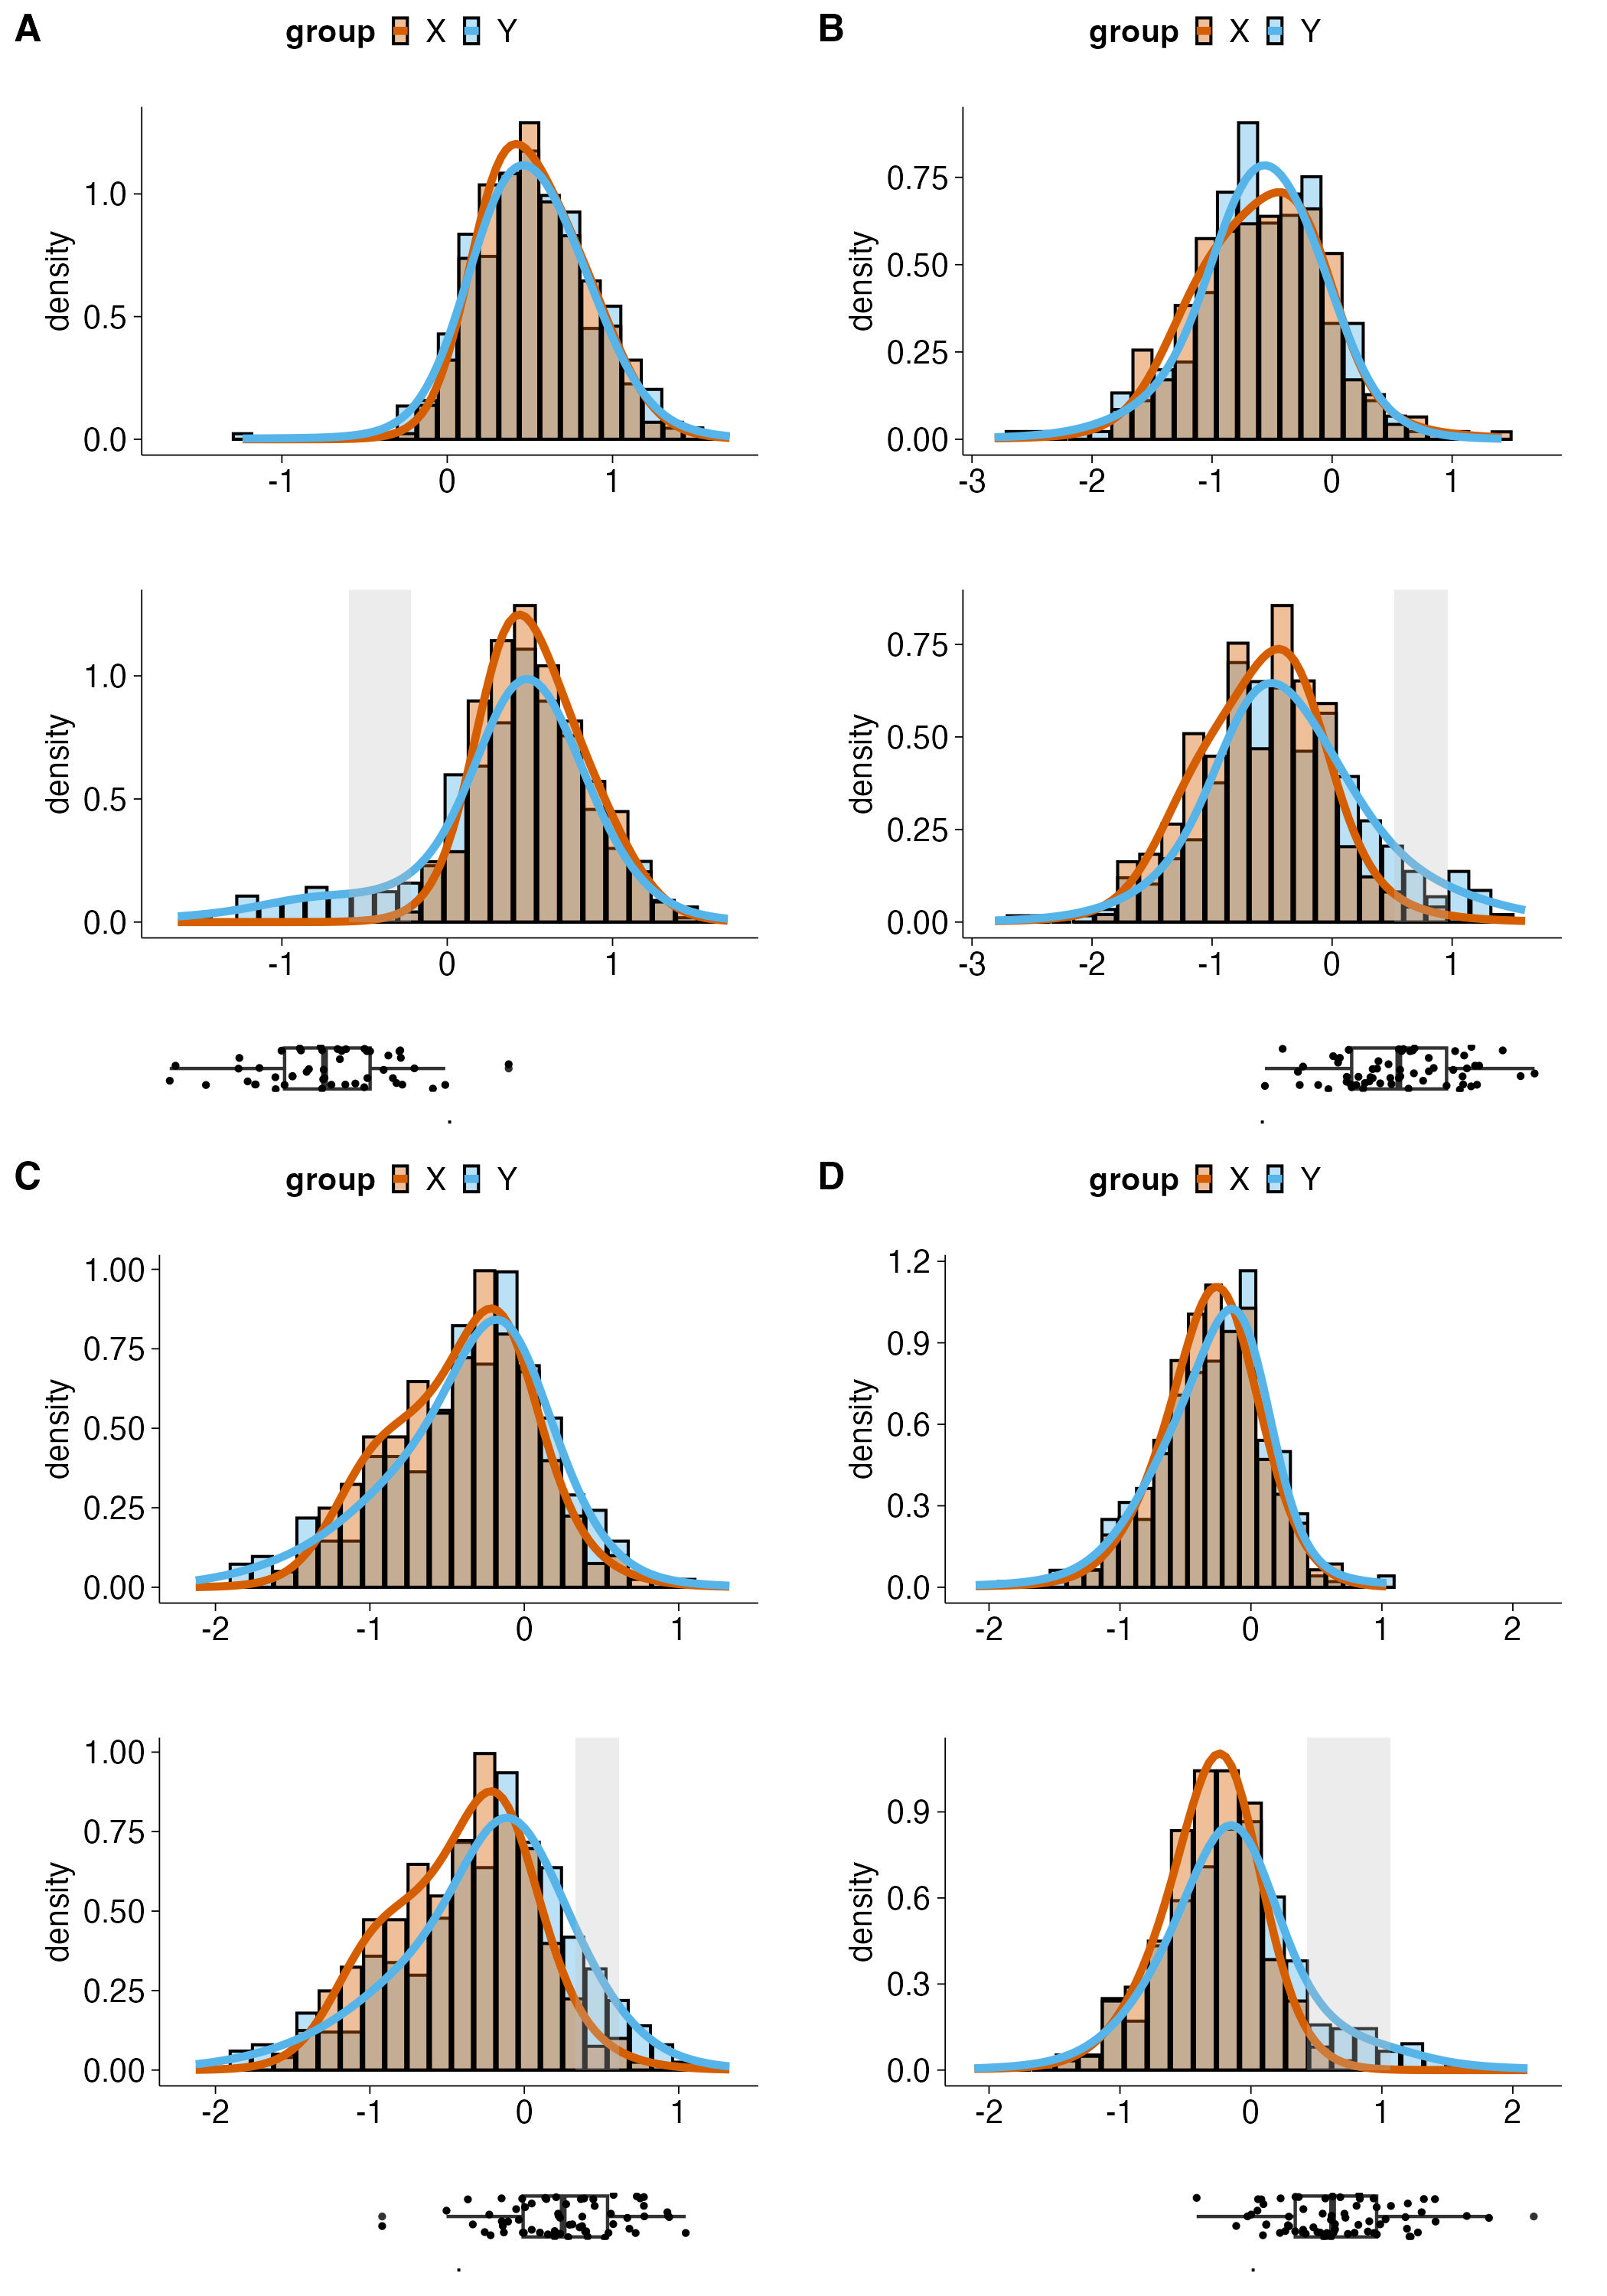
\includegraphics[width=0.85\linewidth]{figs/fig8.jpg}
    \captionsetup{labelfont={bf,small,color=red}}
    \caption{\textbf{\textcolor{red}{gamdid visualizations for four representative features detected by all three methods in the spike-in case study}} Each panel (\textbf{A}--\textbf{D}) shows one feature, following the same layout as the panels of Figure \ref{fig:msqrob_distinct_only}: the mock comparison (top), the comparison after spike-in (middle), and a boxplot indicating where the spike-in melanoma cells are located (bottom). All four features are detected as significant by msqrob2, gamdid, and distinct, forming part of the 52-feature consensus set (see Figure \ref{fig:volanoPlots}C). In all four cases, gamdid's visualization reveals that the distributional difference extends beyond a simple mean shift: these features are DD due to the subpopulation of spike-in cells rather than DA. Moreover, the spiked-in melanoma cells align closely with the detected differential region (gray shading) in each example. This demonstrates that even within the set of features identified by conventional DA methods, gamdid provides additional interpretive value by characterizing how and where the distributions differ. This information is not accessible from the fold change and p-value from a conventional DA method. These examples underscore the broader argument that accounting for full distributional differences, rather than mean shifts alone, leads to richer biological insights.}
    \label{fig:caseStudy_exs}
\end{figure}

\section{Discussion} \label{discussion}

\textbf{Heterogeneity in single-cell data}
Because of \texttt{gamdid}'s flexible approach, it captures the heterogeneity of single-cell data that is, by design, missed by conventional DA methods. In the case study, \texttt{gamdid} identifies three features that are not detected by conventional DA methods as the distributional differences do not involve a sufficiently large mean shift.\\
More importantly, even the 52 features detected by both DA and DD methods further emphasize the need to account for heterogeneity in single-cell data. Indeed, for the majority of these features, the distributional difference extends beyond a pure mean shift. This is illustrated by \texttt{gamdid}'s visualization which reveals the important nuances of these more complex distributional patterns.\\
Four representative examples are provided in Figure \ref{fig:caseStudy_exs}. Notably, in all four examples the detected differential regions align closely with the regions of the distribution where melanoma cells were spiked in, underscoring the utility of \texttt{gamdid}'s visualization.
\\
\\
\textbf{Ranking of significant features}
Notably, the ranking of significant features is of increasing interest in proteomics, and \texttt{gamdid} offers a key advantage in this regard. For DA features, the \texttt{gamdid} ranking is very similar to that of top-performing DA methods (which is not the case for \texttt{distinct}, see Table \ref{tab:only_msqrob2}). Moreover, \texttt{gamdid} can also prioritize interesting features that are completely overlooked by DA methods. This is illustrated in Table \ref{tab:only_gamdid}, which shows that two out of the three features exclusively detected by \texttt{gamdid} are assigned high p-values by \texttt{msqrob2}.
\\
\\
\textbf{Conceptual difference between \texttt{gamdid} and \texttt{distinct}}
The simulation results reflect a fundamental difference in how \texttt{distinct} and the GAM methodology characterize distributional differences between groups. \texttt{distinct} operates on empirical cumulative distribution functions (ECDFs) and quantifies the mean difference between the ECDFs of two groups. By design, this mean ECDF difference is sensitive to sustained, global displacements of probability mass. The GAM-based approach, however, models the density function of each group. Because density estimation is inherently local, the GAM is particularly well-suited to detect distributional changes that are concentrated in specific regions of the distribution.\\
Figure \ref{fig:distinctVSgamdid}A--B illustrates this using a feature from the Petrosius DB simulations that exhibits a local change without substantially displacing the bulk of the probability mass. In this case, the mean difference between the ECDFs of the two groups remains modest, resulting in reduced power for \texttt{distinct}, whereas the GAM-based method is able to successfully identify the differential region.


Conversely, distributional changes like mean shifts produce large, sustained differences between the ECDFs of two groups and are therefore readily detected by \texttt{distinct}. The GAM-based method, however, exhibits reduced power in such settings, as mean shifts constitute diffuse, global changes that do not concentrate in any particular local region of the distribution. This behavior is illustrated in Figure \ref{fig:distinctVSgamdid}C--D, which presents a feature from the Petrosius DE simulations. This example shows an accumulated difference between the ECDFs, while the GAM method is not able to detect differential regions.\\
This motivates the aggregation of GAM-derived p-values with those from \texttt{msqrob2}, which is specifically designed to detect mean shifts with high sensitivity.

\begin{figure}[H]
    \centering
    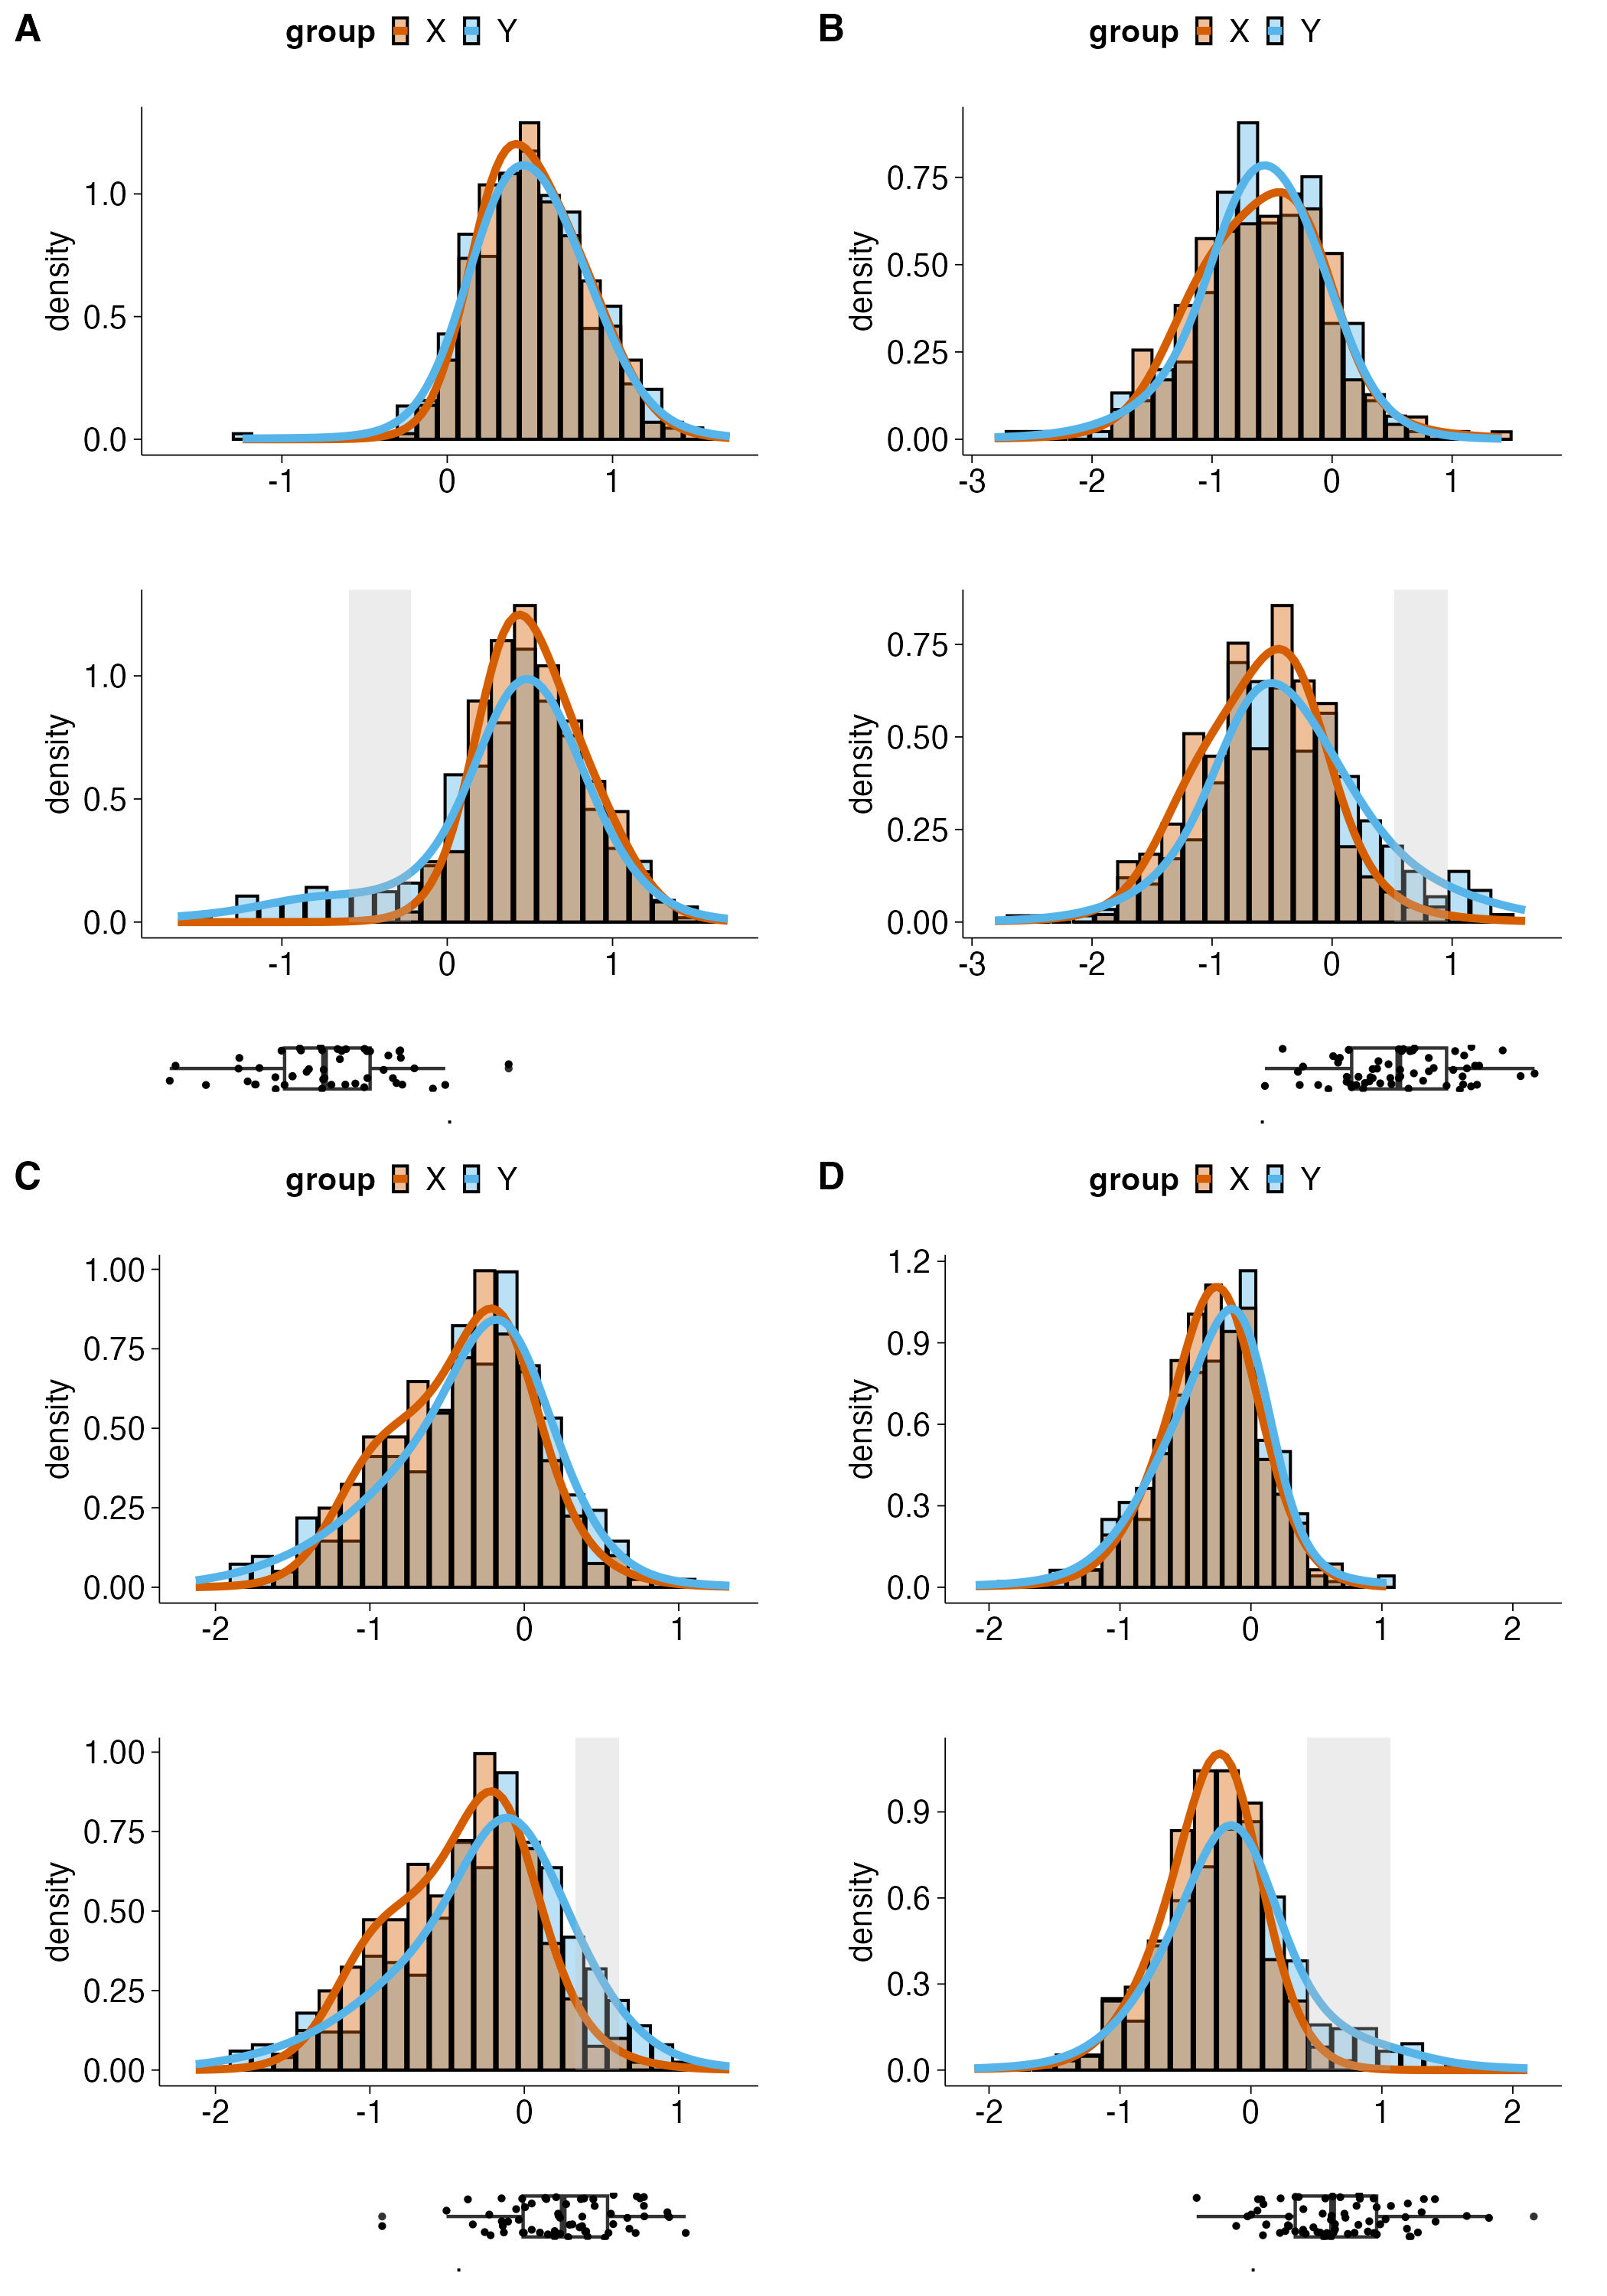
\includegraphics[width=0.85\linewidth]{figs/fig8.jpg}
    \captionsetup{labelfont={bf,small}}
    \caption{\textbf{Conceptual difference between distinct and gamdid} Comparison of how distinct (ECDF curves, top) and gamdid (density visualization, bottom) characterize two features from the Petrosius simulations. \textbf{A--B}: A feature from the DB scenario, detected by gamdid (FDR adjusted p-value = 0.012) and not by distinct (FDR adjusted p-value = 0.278). The mean ECDF difference (used by distinct) between groups is modest (A) because the induced bimodality does not produce a sustained, global displacement of probability mass, while the gamdid visualization (B) reveals the local bimodality clearly and the difference smoother identifies the specific regions where the densities diverge (gray shading). \textbf{C--D}: A feature with a pure mean shift (DE), detected by distinct (FDR adjusted p-value = 0.020) and not by the standalone GAM method before aggregation (FDR adjusted p-value = 0.227). The ECDF curves (C) show a large, sustained horizontal displacement between groups, whereas the GAM fits (D) overlap and show no identifiable differential region, reflecting the GAM's reduced power for diffuse, global distributional changes. distinct is thus more sensitive to sustained, global ECDF displacements, while the GAM's density-based, inherently local approach is better suited to detecting concentrated, shape-based differences. This complementarity motivates the aggregation of GAM p-values with msqrob2 p-values: after aggregation, the DE feature (C--D) is detected by gamdid (FDR adjusted p-value = 0.029).}
    \label{fig:distinctVSgamdid}
\end{figure}


\textbf{P-value aggregation}
The aggregated p-value in \texttt{gamdid} combines the local sensitivity of the GAM with the established power of \texttt{msqrob2} for mean-based inference, ensuring that \texttt{gamdid} is well-suited to detect any form of distributional difference. As expected, a modest loss of power relative to each individual component is observed in scenarios where only one of the two components contributes meaningfully: the DE scenario for the GAM component, and the DV and DB scenarios for \texttt{msqrob2}. This is an inherent consequence of p-value aggregation when one of the contributing p-values carries no signal. In scenarios where the distributional change involves both a mean shift and a difference in shape, however, \texttt{gamdid} combines the strength of both methods and outperforms each method separately, demonstrating the practical benefit of the aggregation strategy.
\\
\\
\textbf{FDR control}
\texttt{gamdid} achieves conservative FDR control at the nominal 5\% threshold throughout all simulations.
\\
\\
\textbf{Computational efficiency}
To evaluate computational efficiency, the runtime of both \texttt{gamdid} and \texttt{distinct} was measured on the spike-in case study dataset, comprising 1316 features and 824 cells. Each method was executed on a single core, and runtimes were averaged across ten independent runs. The mean runtime for \texttt{gamdid} was 16 seconds, whereas \texttt{distinct} required 256 seconds on average, indicating that \texttt{gamdid} achieved a speedup of more than fifteen-fold (see supplementary Figure \ref{fig:runtime}).


This can be attributed to two key factors. First, \texttt{gamdid} does not rely on permutation-based inference as \texttt{distinct} does. Second, as \texttt{distinct} cannot handle missing values, all missing observations must be removed on a per-feature basis prior to analysis.
\\
\\
\textbf{Outlook}
The development of \texttt{gamdid} represents a significant advance toward a more comprehensive interpretation of the information in single-cell proteomics data. By extending differential analysis beyond mean-based comparisons, \texttt{gamdid} enables the systematic investigation of distributional changes and thereby facilitates a more detailed characterization of cellular heterogeneity. This functionality uncovers biologically relevant variation that has remained largely unexplored by existing data analysis frameworks.\\
As single-cell proteomics technologies continue to mature and datasets grow in size and complexity, the ability to detect and interpret subtle distributional differences will become increasingly important. We therefore anticipate that \texttt{gamdid} can find applications not only in the comparison of cell types and conditions, but also in the identification of subpopulations, or the characterization of transitional cell states.\\
More broadly, the framework presented here is not intrinsically limited to proteomics and could, in principle, be adapted to other single-cell modalities, including single-cell transcriptomics, metabolomics and flow cytometry, where distributional heterogeneity likewise constitutes an important source of biological information. As such, \texttt{gamdid} has the potential to support a broader methodological shift toward distributional approaches in single-cell data analysis, enabling a more comprehensive characterization of cellular variation beyond changes in average abundance levels.


%The \texttt{msqrob2} analysis is slightly too liberal in the Leduc dataset, which is likely attributable to correlation between the proteins.


%\textbf{Leduc vs Petrosius}
%All methods exhibit reduced performance in the Petrosius simulations relative to the Leduc simulations. And interestingly, the performance gap is more pronounced, with \texttt{gamdid} substantially outperforming \texttt{distinct} on the Petrosius dataset.\\
%This difference is primarily attributable to the smaller sample size in the Petrosius dataset, which negatively impacts the permutation-based inference of \texttt{distinct}, as a limited number of permutations reduces the resolution of the resulting null distribution.\\
%To evaluate this, we subsampled the Leduc dataset such that the average number of non-missing observations per group over all feature matched that of the Petrosius dataset. The resulting FDP-TPP curves, shown in figure \ref{fig:leducsims_gamdid_subsample}, demonstrate similar trends as those observed in the Petrosius simulations. Most notably, this confirms that \texttt{gamdid} exhibits higher power than \texttt{distinct} under small-sample conditions, which has practical implications for the analysis of single-cell proteomics datasets where the number of cells per condition is limited.

%\begin{figure}[H]
%    \centering
%    \includegraphics[scale=0.2]{figs/fig17.jpg}
%    \caption{\textbf{Subsample simulation results for \texttt{gamdid}} fdp-tpp curves for \texttt{gamdid} and \texttt{distinct} for comparing two groups in the Leduc dataset under different simulations scenarios after subsampling}
%    \label{fig:leducsims_gamdid_subsample}
%\end{figure}

\section{Methods} \label{methods}
{\color{red}

Below, we first outline the \texttt{gamdid} approach (model equations,
test statistics and the simultaneous confidence bands are discussed in
more detail in the Supplementary materials).
We subsequently describe the covariate adjustment procedure, the datasets,
the simulation framework and the implementation.

\subsection{Overview of the gamdid approach}

The analysis is performed for each feature (protein or peptide) separately and
consists of five steps (see Figure \ref{fig:workflow}).
\\
\\
\textbf{Step 1: Estimating a smooth distribution per group}
For a given feature, the abundance values of all cells are binned into a histogram,
using the same bins for every group (see Figure \ref{fig:workflow}, panel A).
Following Lindsey \cite{lindsay_method} and Efron \cite{efron}, the bin counts
can be treated as Poisson counts.
\\
We then model the bin counts as a function of the bin midpoints using a
Poisson GAM, which allows us to flexibly model the
shape of the distribution with a smooth curve. Each group receives its own
smooth curve (see Figure \ref{fig:workflow}, panel B).
Equation \ref{eq:GAM_simple} schematically represents the smooth curve for group $c$
and bin $k$ with midpoint $mid_k$.
\begin{equation}
    \log(\text{expected count}_{ck}) = \underbrace{f_c(mid_k)}_{\text{density estimation for group } c} + \text{normalization offset}_c
    \label{eq:GAM_simple}
\end{equation}
where $f_c$ is a flexible smooth function that captures the shape of the distribution of group $c$.
The counts are normalized using an offset, which allows us to interpret the curves
as densities.
\\
\\
\textbf{Step 2: Testing whether the distributions differ}
If two groups have the same distribution, their smooth curves are identical,
i.e. $H_0: f_{c_1} = f_{c_2}$. We test this by assessing if
the parameters corresponding to a smooth curve $\beta_{f_c}$
differ between the groups, i.e. $H_0: \beta_{f_{c_1}} = \beta_{f_{c_2}}$.
We do this by employing a Wald-type test that builds on the work of Wood \cite{Wald}.
The resulting p-value, referred to as the GAM p-value, captures any difference in
distribution between the groups: mean shifts, differences in variance, modality,
skewness...
\\
\\
\textbf{Step 3: Combining with a mean-shift test}
Because the GAM test spreads its power over all possible types of distributional
differences,
it is less powerful than a dedicated DA method for detecting pure mean shifts.
We therefore also compute a p-value with \texttt{msqrob2}, a robust linear-model
approach designed for detecting mean shifts in proteomics data \cite{msqrob}.
The GAM and
\texttt{msqrob2} p-values are combined into a single 'feature-level aggregated
p-value' using the harmonic mean p-value (HMP) method \cite{harmonicp}.
As a result, \texttt{gamdid} largely retains the
sensitivity of conventional DA analysis for mean shifts, while additionally
detecting changes in distributional shape that DA methods miss.
\\
\\
\textbf{Step 4: Multiple testing and pairwise comparisons}
The feature-level aggregated p-values are corrected for multiple testing across
features using the Benjamini-Hochberg FDR procedure
\cite{BH_procedure}. When more than two groups are compared, significant features
are followed up with pairwise comparisons between all pairs of groups, using the
same combination of GAM and \texttt{msqrob2} tests. The feature-level and pairwise
hypotheses are jointly controlled for multiple testing by the stagewise testing
procedure \cite{stagewise_testing, stager}.
\\
\\
\textbf{Step 5: Detecting differential regions}
Finally, \texttt{gamdid} can indicate where the
distributions differ. For this, a log-difference smoother is computed. This
smoother displays the difference between the estimated log-densities of two
groups, together with a simultaneous confidence band. Regions where this
band excludes zero indicate a statistically significant local distributional
difference; these are marked by gray shading (Figure \ref{fig:workflow}, panel C).
}

\subsection{Covariate adjustment}
In addition to the covariate of interest, \texttt{gamdid} allows users to account
for confounding variables through a nuisance formula, enabling applications such
as batch correction in multi-batch experimental designs. Both the covariate of
interest and the nuisance formula are combined into one model in the \texttt{msqrob2}
analysis, and an appropriate contrast is constructed to test for distributional
differences in the covariate of interest.\\
To remove the influence of nuisance covariates from the GAM-based inference,
partial residuals with respect to the covariate of interest are computed from
the \texttt{msqrob2} fit and subsequently used as input to the GAM analysis.
This two-step approach is required due to the binning strategy: as a single bin
may contain observations that correspond to different groups of the nuisance
covariate, direct covariate adjustment within the GAM framework is not feasible.\\
Note, however, that the uncertainty associated with the regression of the nuisance
covariates in the first step is not accounted for, so the resulting p-values should be
interpreted with caution.

\subsection{Data}
\begin{itemize}
    \item \texttt{leduc2022\_pSCoPE}: These data were acquired using pSCoPE technology: a TMT-18plex protocol with prioritized data-dependent acquisition (DDA) carried out by a Thermo Scientific Q-Exactive mass spectrometer \cite{leduc}. The MS data were identified and quantified using MaxQuant version 1.6.17 \cite{maxquant}. We performed quality control by filtering low-quality features and filtering cells with a median coefficient of variation greater than 0.6, calculated using the \textit{medianCVperCell} function of the \texttt{scp} package \cite{scp_paper}. The PSM intensities were log2-transformed for variance-stabilization, median centered and summarized to the protein level using median summarization per MS run. Subsequently, samples were normalized through median centering and proteins with more than 95\% missingness were filtered out, resulting in a dataset with 776 melanoma cells and 755 monocytes profiled across 2120 proteins.
    \item \texttt{petrosius2023\_mES}: These data originate from a label-free SCP experiment conducted on mouse embryonic stem cells cultured under two distinct conditions: a serum-free 2i condition (m2i) containing cytokine LIF and inhibitors targeting the MEK and GSK3 pathways, and a serum condition (m15) only containing cytokine LIF \cite{petro}. Data acquisition was performed using an Orbitrap Eclipse Tribrid mass spectrometer operating in data-independent acquisition (DIA) mode. The resulting mass spectrometry data were subsequently analyzed by the authors using Spectronaut v17 \cite{spectronaut}.
    We performed quality control by removing cells with fewer than 500 detected peptides or a median intensity lower than 11. Features with more than 95\% missing values were also removed. The detected intensities were log2-transformed for variance-stabilization, and the intensities of each cell were centered with the median log2-intensity of the corresponding cell. Subsequently, peptides were summarized to the protein level through median polish summarization. The resulting dataset contains 295 m15 and 269 m2i cells with 2492 proteins.
\end{itemize}
Preprocessed protein-level summarized assays from both datasets served as the foundation for our simulations. From the Petrosius dataset, we selected the 269 m2i-condition cells, while from Leduc, we selected the 755 monocytes (in both cases following removal of non-informative cells during preprocessing). Within each selected subset, no systematic biological differences are expected between cells. Consequently, random assignment of cells to two mock groups (A and B) yields a dataset suitable as a mock basis for a controlled two-group comparative analysis.

\subsection{Simulation framework}
The benchmark simulations are based on protein-level mock data from both the Leduc and Petrosius datasets, as described in the Results section. For each dataset, mock groups A and B were formed by random assignment of cells, and distributional signal was introduced in group B for 20\% of randomly selected features. Five types of distributional signal were considered, following the framework of Korthauer et al. (2016) \cite{scdd}:
\begin{itemize}
    \item \textbf{DE:} A shift equal to 40\% of the feature's standard deviation is added to all observations in group B.
    \item \textbf{DV:} Independent Gaussian noise with mean zero and standard deviation equal to 120\% of the feature's standard deviation is added to all observations in group B, thereby increasing the spread of the distribution without altering its mean.
    \item \textbf{DB:} For 50\% of the observations in group B, a value of 90\% of the feature's standard deviation is added; for the remaining 50\%, the same value is subtracted. This induces a bimodal distribution in group B.
    \item \textbf{DM:} A value of 90\% of the feature's standard deviation is added to 50\% of the observations in group B, creating an asymmetric shift concentrated in one tail.
    \item \textbf{DP:} In both groups, observations are split into two subpopulations that are shifted upwards or downwards by 100\% of the feature's standard deviation. In group A, 40\% of the observations are shifted upwards and the remaining 60\% downwards; in group B, 70\% are shifted upwards and 30\% downwards. Both groups are therefore bimodal with identical component locations but different mixing proportions, which also results in a difference in group means of 0.6 standard deviations. In the three-group simulations, group C is treated identically to group A.
\end{itemize}


\subsection{Implementation}
The methods for assessing differential distributions are implemented in the \texttt{gamdid} R package that is publicly available through GitHub (github.com/statOmics/gamdid) and will be submitted to Bioconductor.\\
\texttt{gamdid} builds upon the CRAN packages \texttt{mgcv} \cite{mgcv} and \texttt{harmonicmeanp} \cite{hmp_package} for fitting generalized additive models and p-value aggregation; and on the R/Bioconductor packages \texttt{stageR} \cite{stager} for stagewise testing and \texttt{msqrob2} for detecting shifts in mean abundance \cite{msqrob}. Specifically, \texttt{mgcv} version 1.9.4, \texttt{harmonicmeanp} version 3.0.1, \texttt{stageR} version 1.32.0 and \texttt{msqrob2} version 1.18.0 were used in R version 4.5.3.


\section{Data Availability}
All data used in this manuscript are publicly available\textcolor{red}{; no new mass spectrometry data were generated}. The Leduc \cite{leduc} and Petrosius \cite{petro} datasets were downloaded using the \texttt{scpdata} \textcolor{red}{\cite{scp_paper, scp_replication}} package from Bioconductor. \textcolor{red}{Leduc: Slavov laboratory website (\url{https://scp.slavovlab.net/Leduc_et_al_2022}) and MassIVE MSV000089159. Petrosius: MassIVE MSV000092429 and Zenodo (\url{https://zenodo.org/records/8146605}).}

\section{Code Availability}
All code used to prepare and analyze the datasets and produce the figures of this manuscript is available through GitHub (github.com/statOmics/gamdid).
Finally, \texttt{gamdid} is published as an open source R-package available through GitHub (github.com/statOmics/gamdid) and will be submitted to Bioconductor.

\section{Acknowledgements}
This work was supported by grants from Ghent University Special Research Fund [BOF20/GOA/023] (S.V., L.C., C.V.), [BOF21/GOA/033] (L.M.) and [BOF/PDO/2025/018] (L.C., C.V.), Research Foundation Flanders [FWO G062219N] (S.V., L.C.), [G071326N] (L.C.), [G010023N, G028821N] (L.M.) and as WOG [W005325N] (L.M. and L.C.), funding from the European Union’s Horizon 2020 Program [101080544 and 101191739] (L.M.).

\newpage

\newpage
\section{Supplementary materials} \label{supplementary}

\renewcommand{\thefigure}{S\arabic{figure}}
\setcounter{figure}{0}

\renewcommand{\thetable}{S\arabic{table}}
\setcounter{table}{0}



\begin{figure}[H]
    \centering
    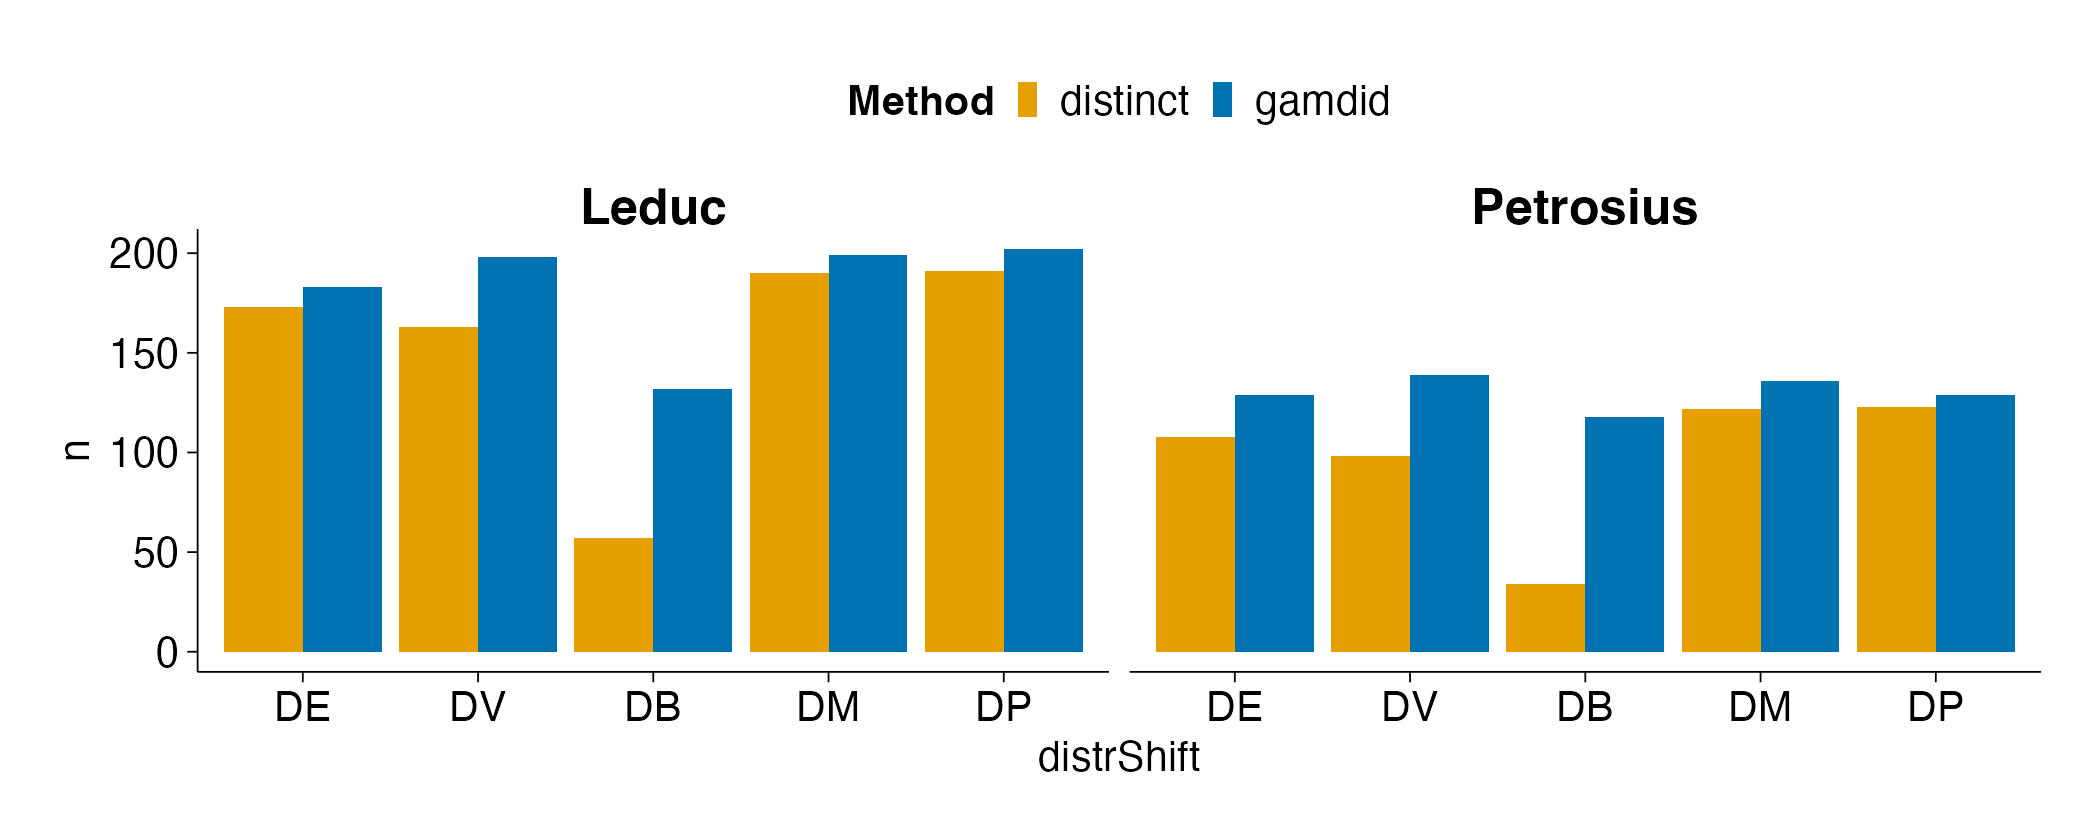
\includegraphics[width=0.85\linewidth]{figs/figS1.jpg}
    \captionsetup{labelfont={bf,small,color=red}}
    \caption{\textbf{\textcolor{red}{Absolute true positive counts for gamdid and distinct at 5\% FDR}} Bar charts displaying the number of true positives recovered at the nominal 5\% FDR threshold for gamdid and distinct across the five simulation scenarios in the Leduc dataset (left) and the Petrosius dataset (right). gamdid recovers a comparable or greater number of true positives in all scenarios, with the largest absolute gains in the DV and DB scenarios (shape-only differences). The false positive counts (Figure \ref{fig:FP}) are similarly low for both methods.}
    \label{fig:TP}
\end{figure}

\begin{figure}[H]
    \centering
    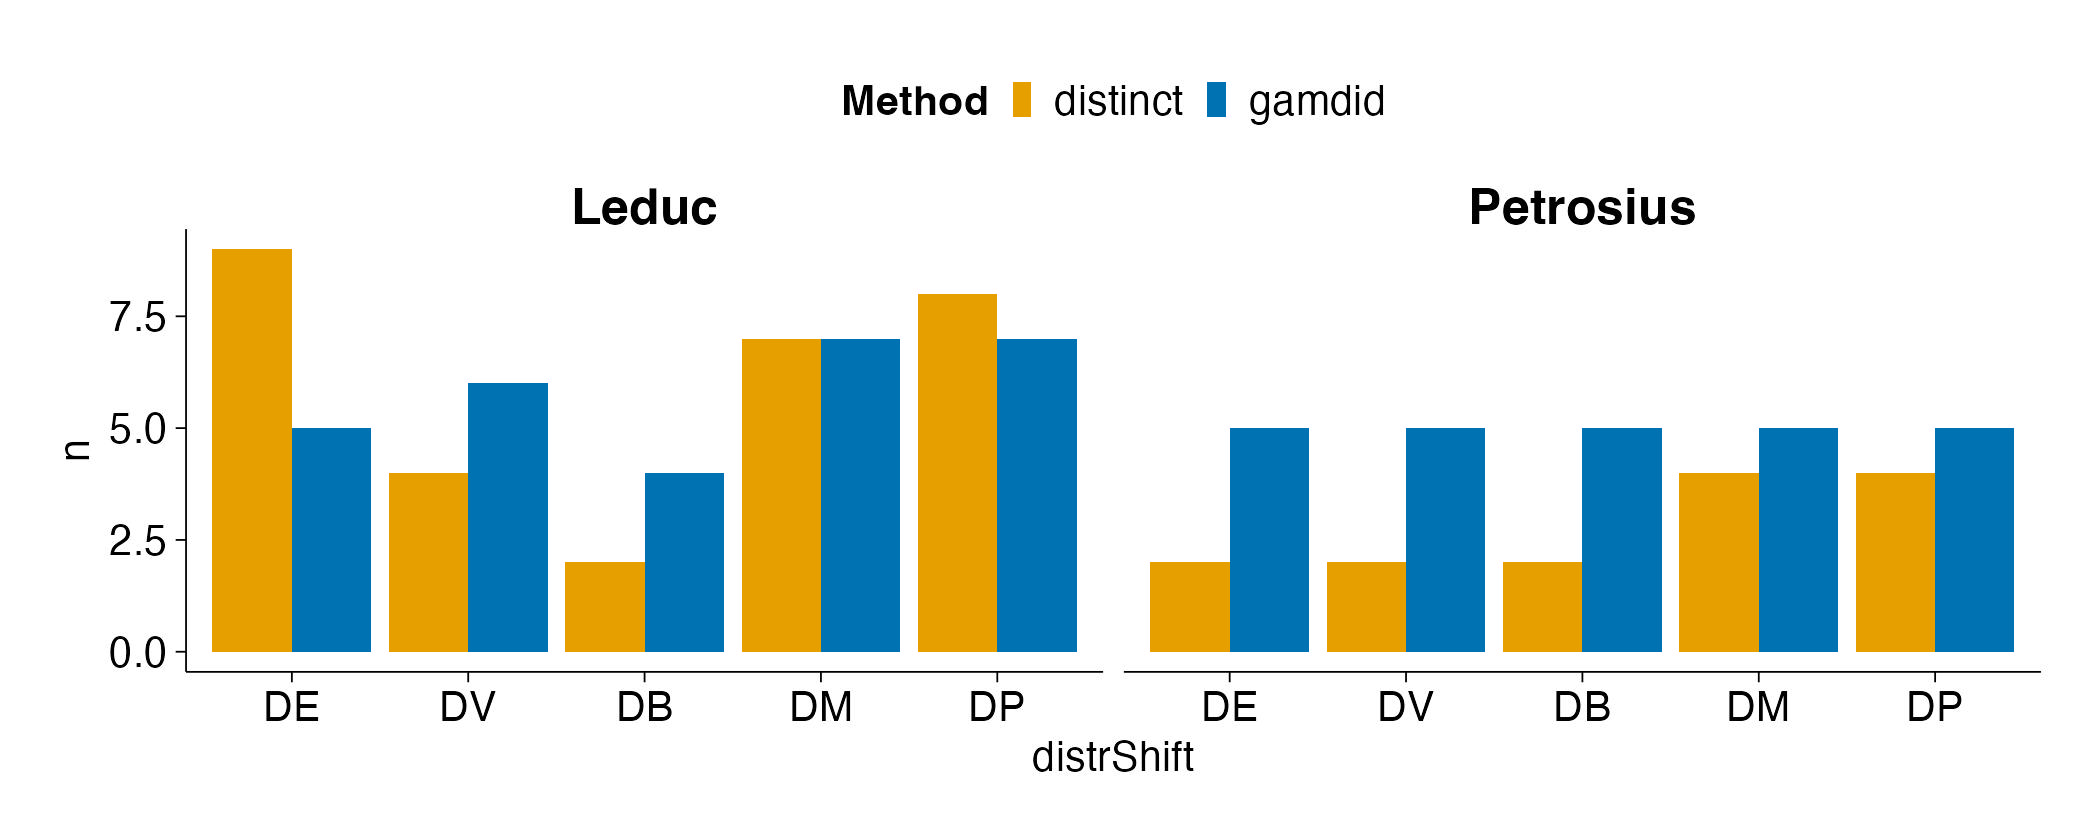
\includegraphics[width=0.85\linewidth]{figs/figS2.jpg}
    \captionsetup{labelfont={bf,small,color=red}}
    \caption{\textbf{\textcolor{red}{Absolute false positive counts for gamdid and distinct at 5\% FDR}} Bar charts displaying the number of false positives at the nominal 5\% FDR threshold for gamdid and distinct across the five simulation scenarios in the Leduc dataset (left) and the Petrosius dataset (right). Both methods maintain similarly low false positive counts across all scenarios in both datasets, confirming that the gains in true positive recovery demonstrated for gamdid in Figure \ref{fig:TP} are not accompanied by inflation of false discoveries.}
    \label{fig:FP}
\end{figure}

\begin{figure}[H]
    \centering
    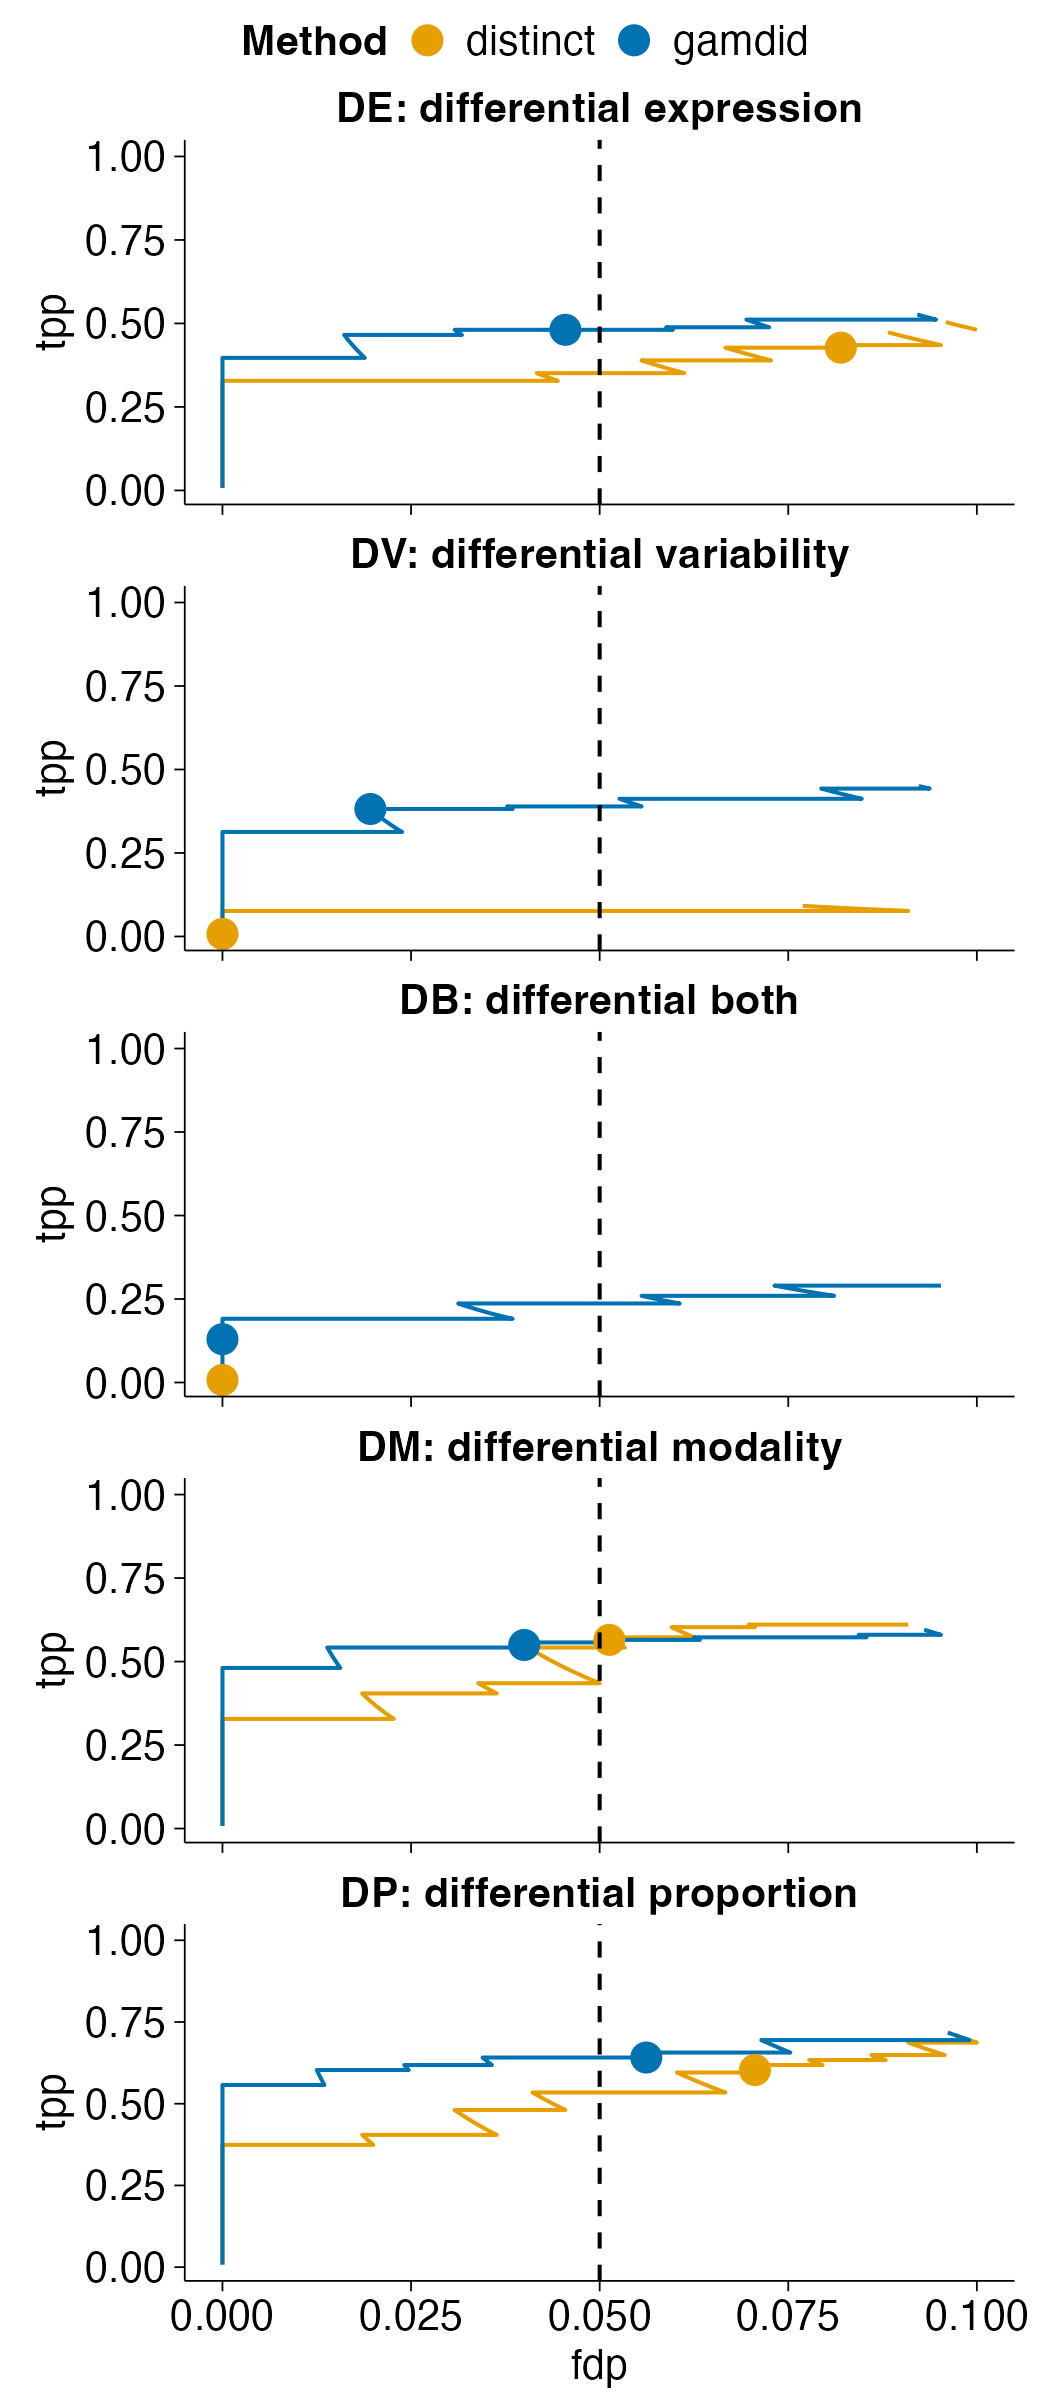
\includegraphics[width=0.425\linewidth]{figs/figS3.jpg}
    \caption{\textbf{Performance of gamdid on a subsampled Leduc dataset} FDP-TPP curves comparing gamdid and distinct across the five simulation scenarios, based on the protein-level mock data of a subsampled version of the Leduc dataset, in which cells were subsampled such that the average number of non-missing observations per group matched that of the Petrosius dataset. The dots mark the 5\% FDR threshold and the dashed vertical line marks FDP = 0.05. This analysis directly tests whether the more pronounced improvements of gamdid over distinct observed in the Petrosius dataset (see the right column of Figure \ref{fig:leducsims_gamdid}) are attributable to the smaller sample size. The results support this hypothesis: under reduced sample size, the performance gap between gamdid and distinct increases. distinct likely suffers from reduced null distribution resolution when fewer observations are available. DB (differential both) denotes a difference in both modality and component means.}
    \label{fig:leducsims_gamdid_subsample}
\end{figure}

\begin{figure}[H]
    \centering
    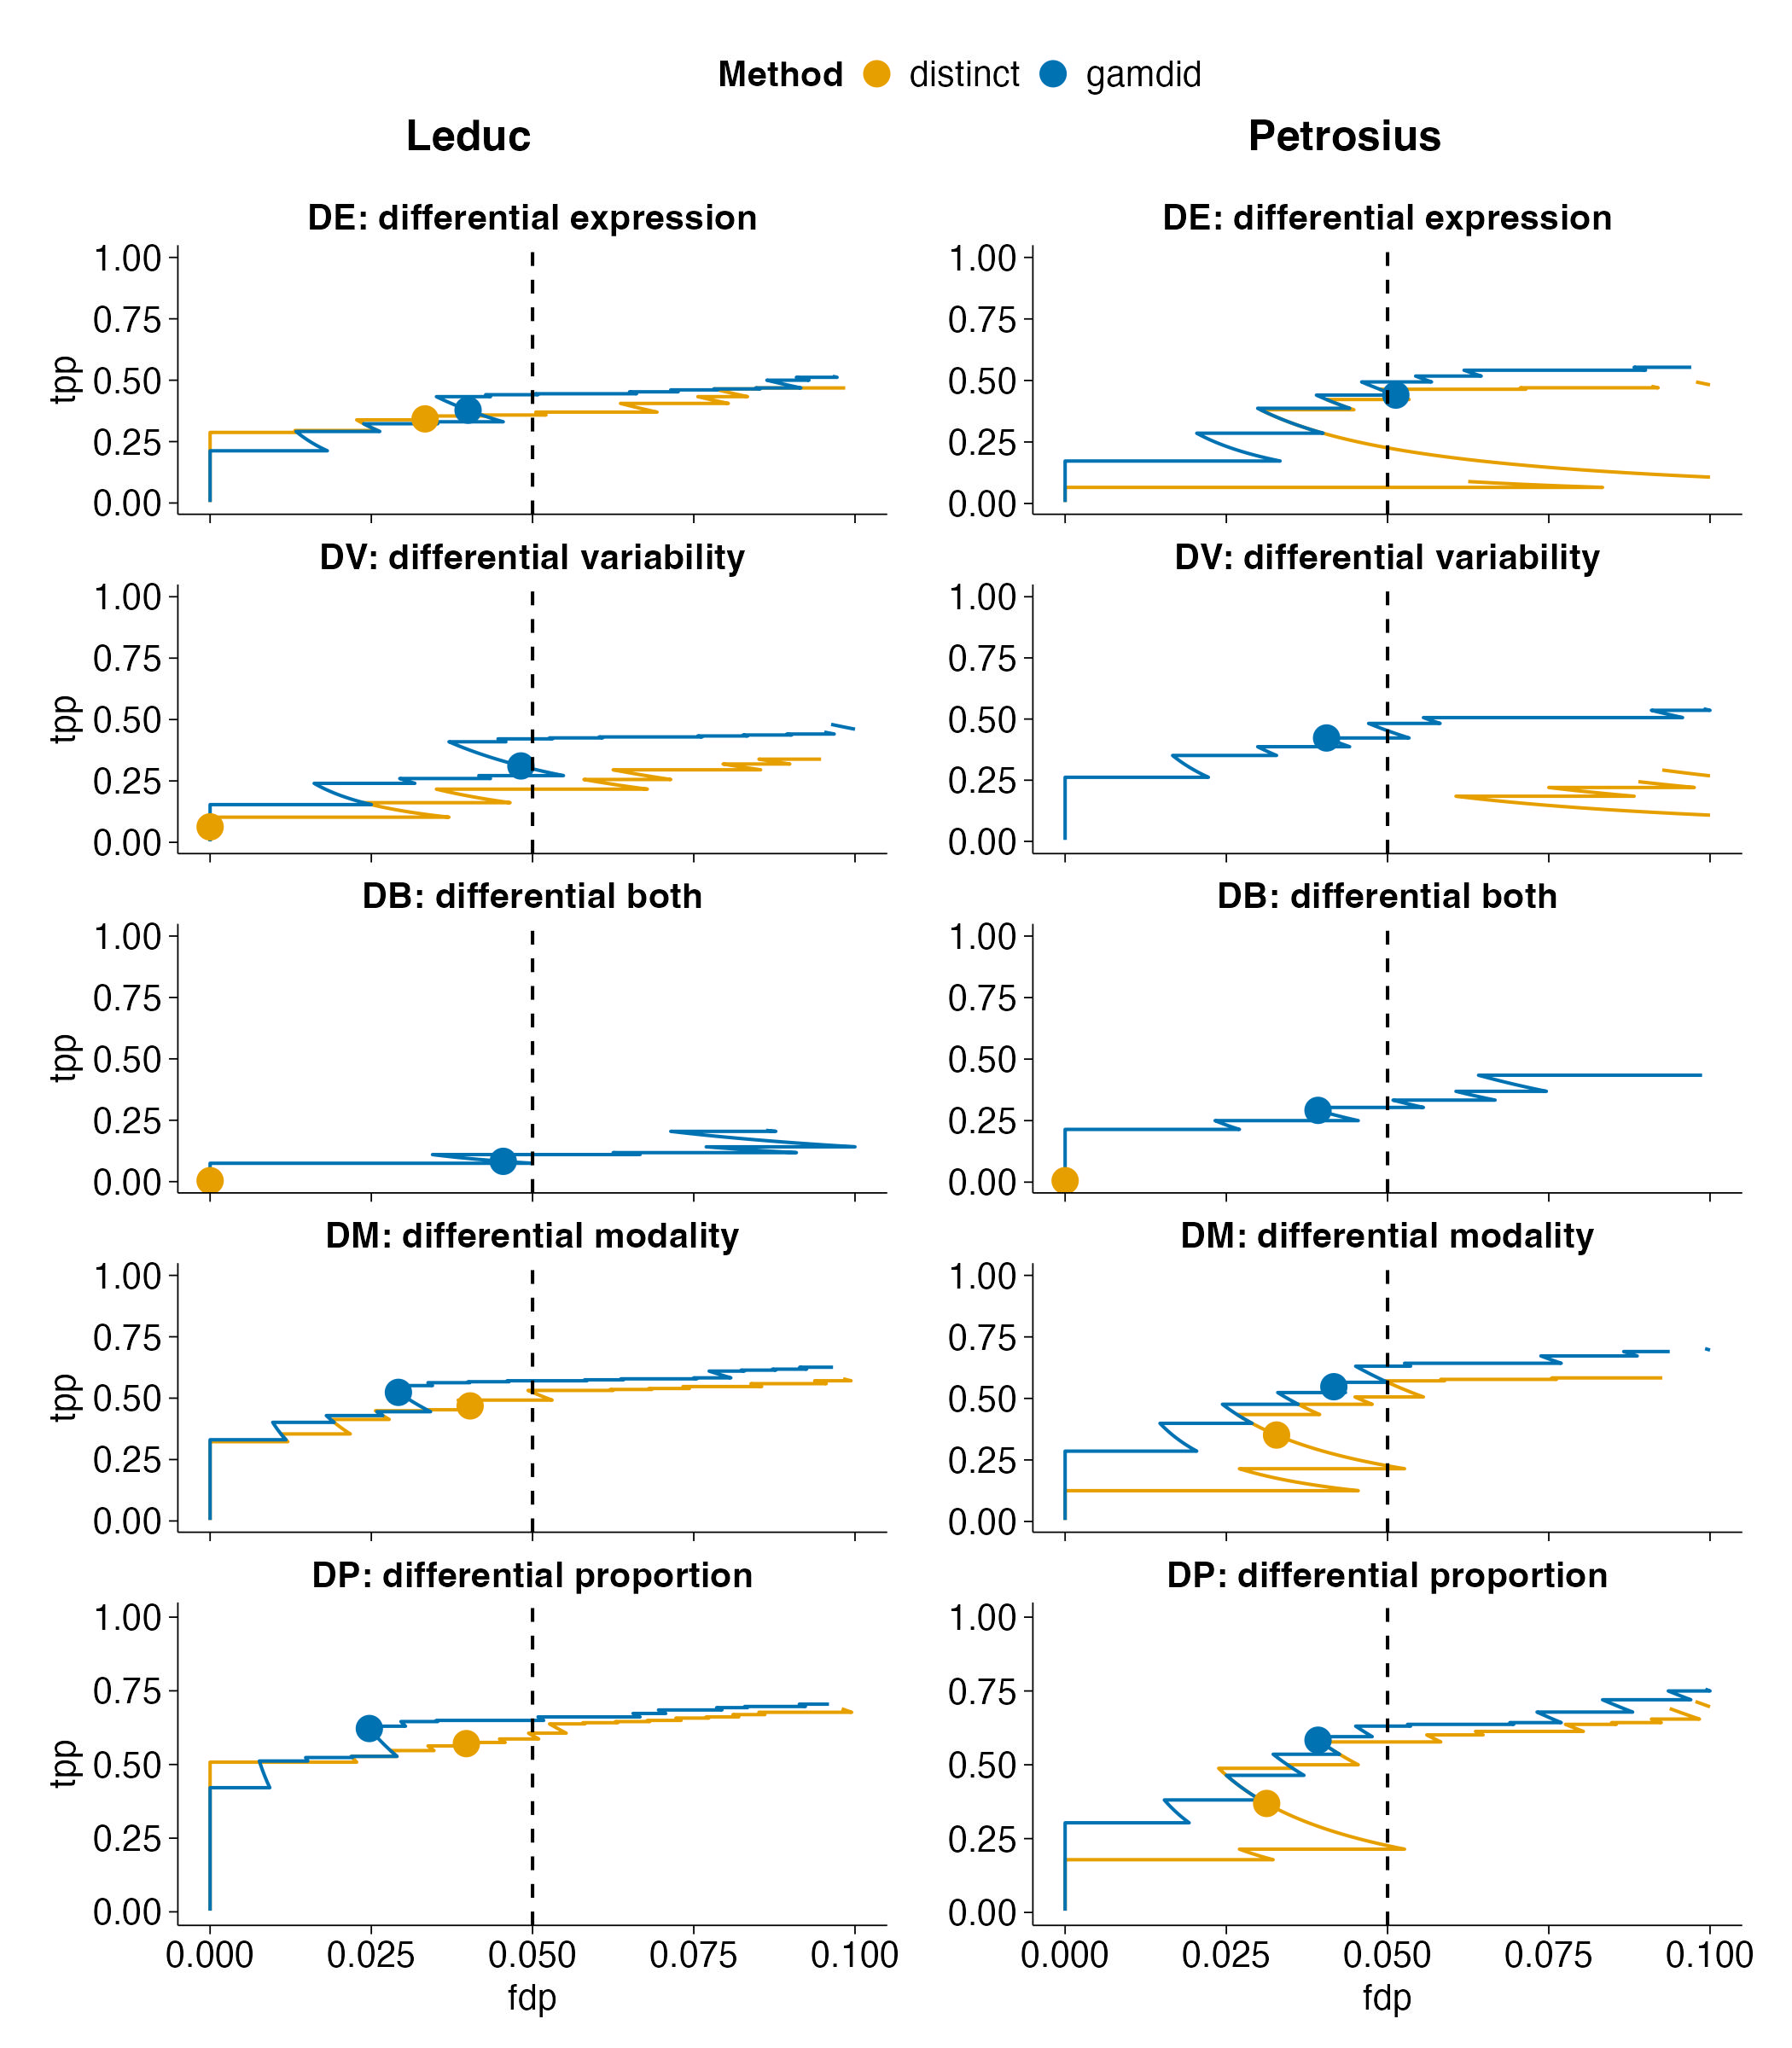
\includegraphics[width=0.85\linewidth]{figs/figS4.jpg}
    \captionsetup{labelfont={bf,small,color=red}}
    \caption{\textbf{\textcolor{red}{Performance of gamdid under reduced signal magnitude}} FDP-TPP curves comparing gamdid and distinct across the five simulation scenarios, based on the protein-level mock data of the Leduc dataset (left; 755 monocytes) and the Petrosius dataset (right; 269 m2i cells), under simulation scenarios with 25\% reduced signal magnitudes (DE: a shift of 30\% instead of 40\% of the feature's standard deviation was used; DV: random Gaussian noise with a standard deviation of 90\% of the feature's standard deviation was added instead of 120\%; DM and DB: a shift of 70\% of the feature's standard deviation was used instead of 90\%, and for DP 75\% instead of 100\%). The dots mark the 5\% FDR threshold and the dashed vertical line marks FDP = 0.05. This analysis assesses whether gamdid's performance advantages are robust to weaker signals that may be encountered in practice. The results are consistent with the original simulations (Figure \ref{fig:leducsims_gamdid}): gamdid controls the FDR at or below the nominal level and retains its advantages for shape-based distributional changes (DV, DB), while remaining competitive with distinct for scenarios where location shifts are involved. The relative improvements over distinct are more pronounced in the Petrosius dataset, consistent with gamdid's advantage under smaller sample sizes. As expected, the reduced signal does lower the overall power of both methods. DB (differential both) denotes a difference in both modality and component means.}
    \label{fig:leducsims_lower_gamdid}
\end{figure}


\begin{figure}[H]
    \centering
    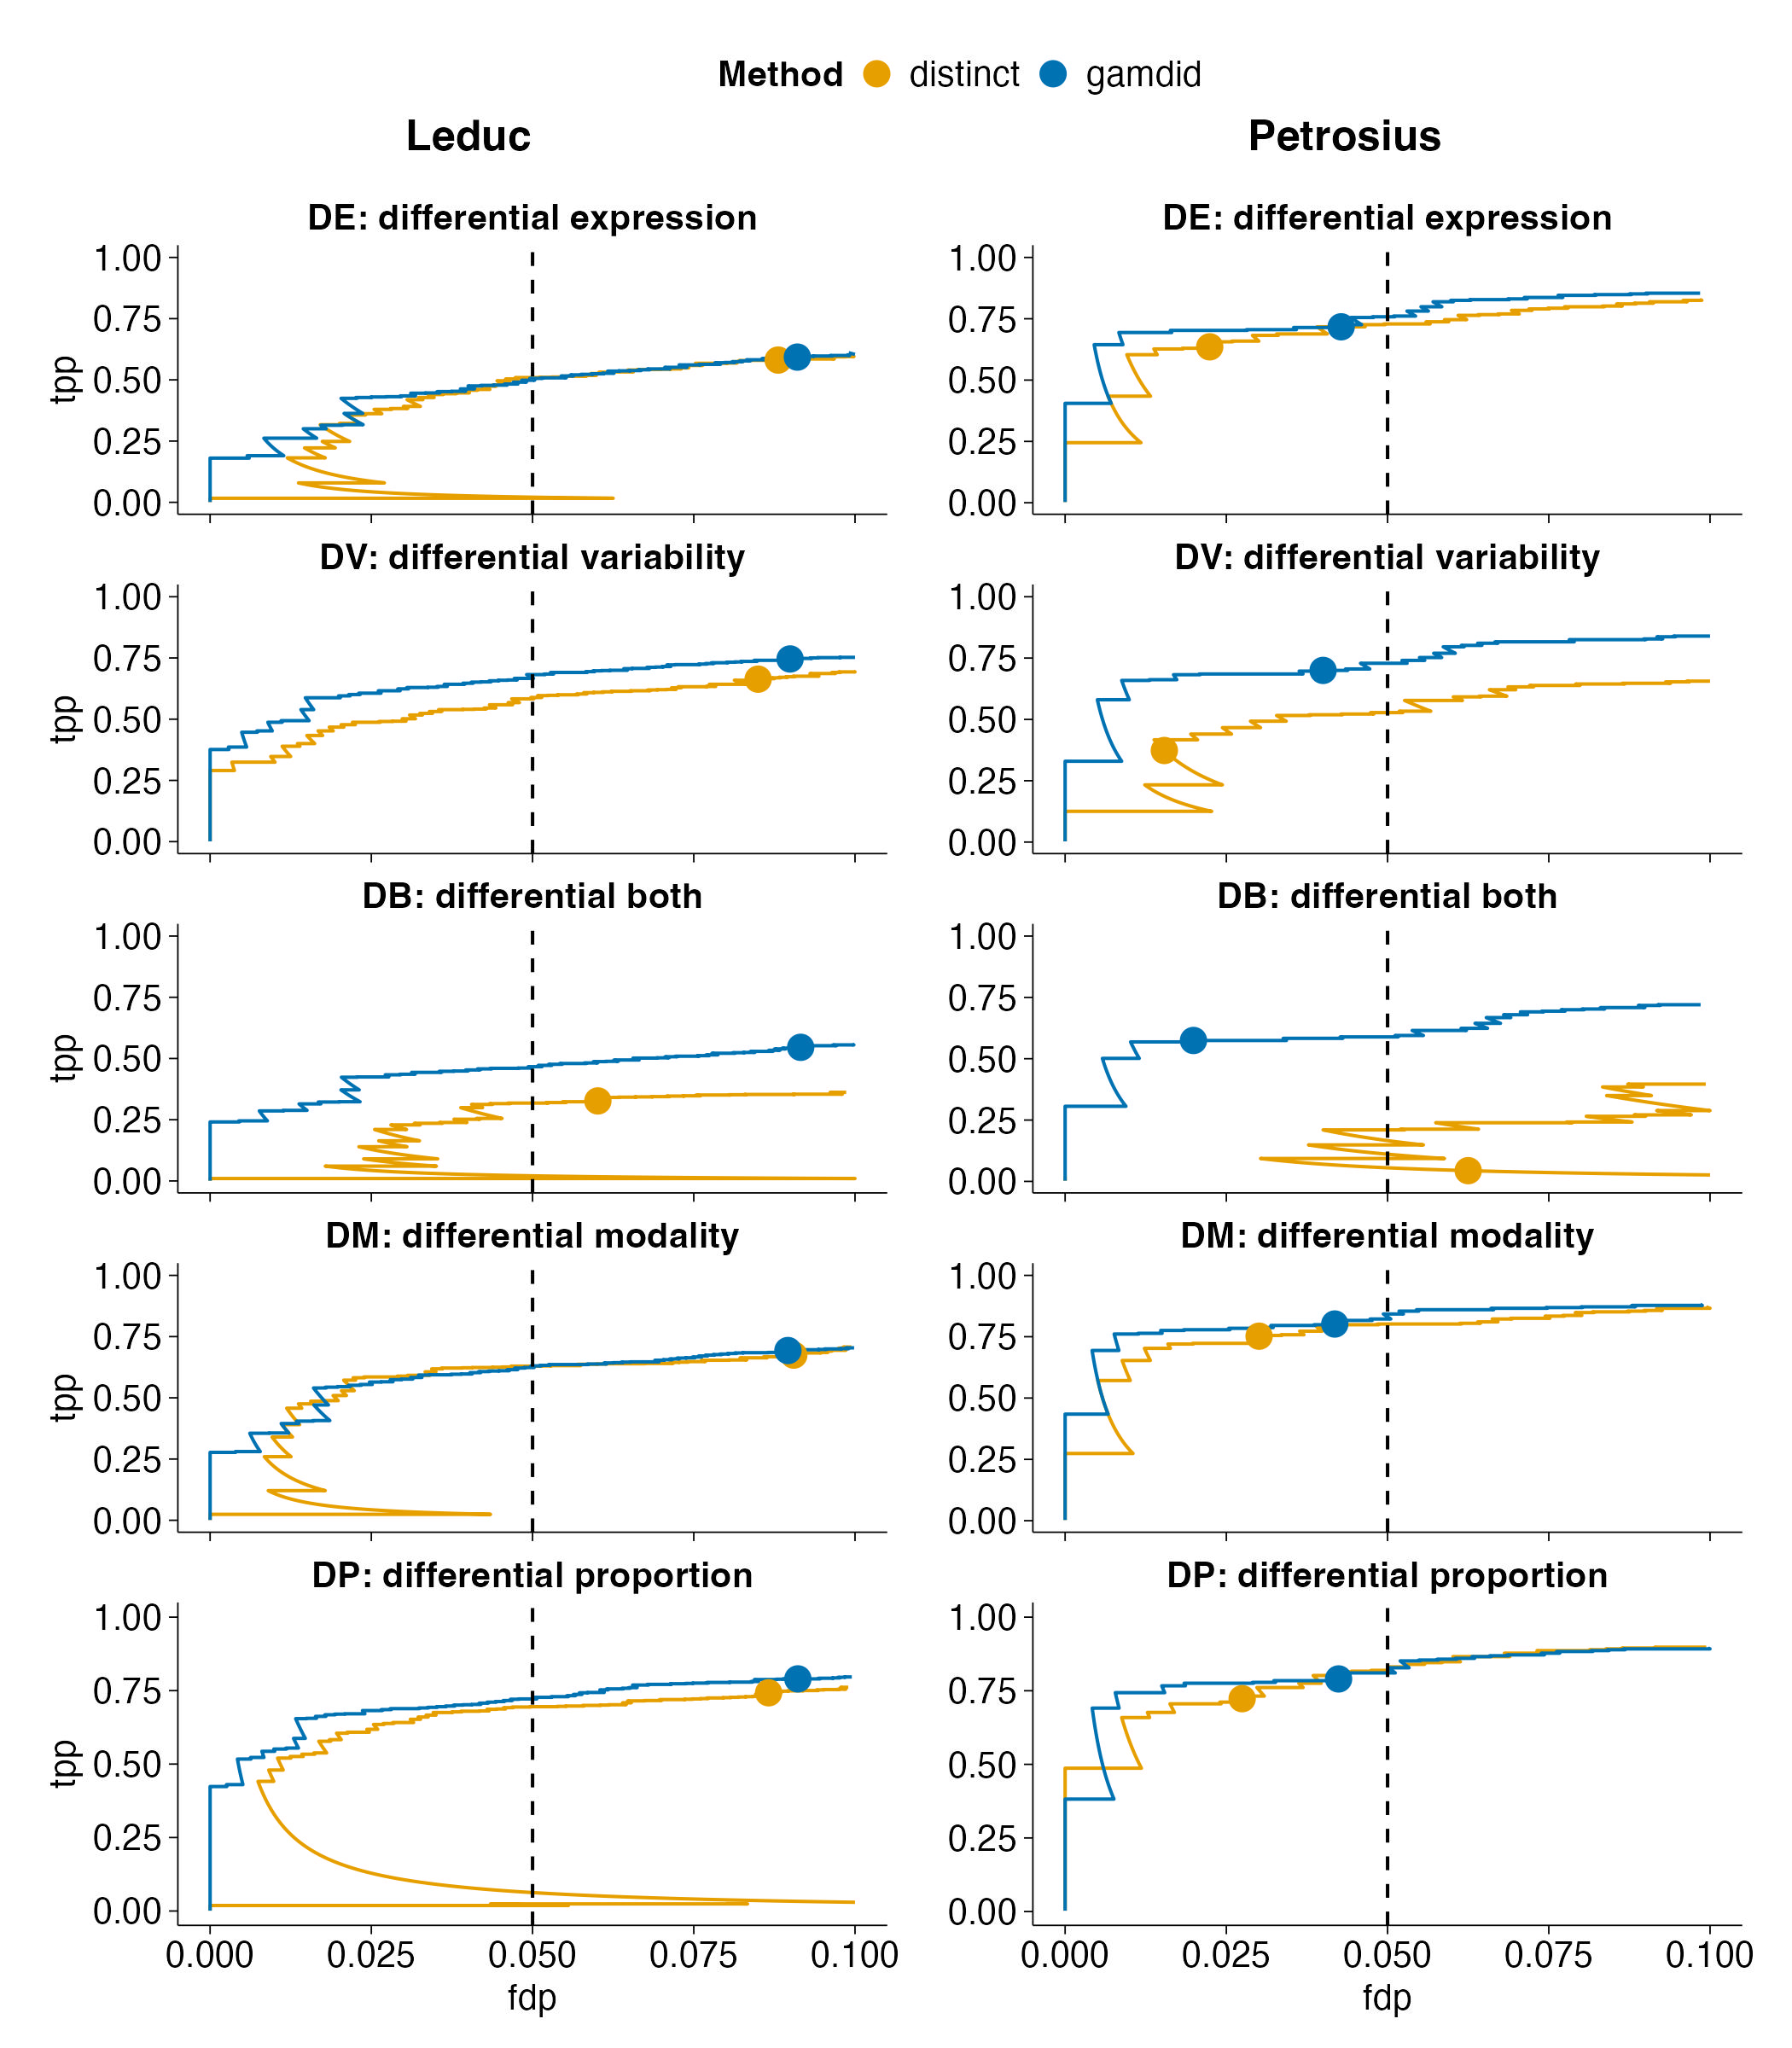
\includegraphics[width=0.85\linewidth]{figs/figS5.jpg}
    \captionsetup{labelfont={bf,small,color=red}}
    \caption{\textbf{\textcolor{red}{Performance of gamdid on peptide-level data}} FDP-TPP curves comparing gamdid and distinct across the five simulation scenarios, based on the peptide-level mock data of the Leduc dataset (left; 755 monocytes) and the Petrosius dataset (right; 269 m2i cells), rather than the protein-level summarized data used in the main analyses. The dots mark the 5\% FDR threshold and the dashed vertical line marks FDP = 0.05. The results are largely consistent with the protein-level findings (Figure \ref{fig:leducsims_gamdid}), and gamdid retains its performance advantages. In the Leduc dataset, FDR control is less conservative at the peptide level than at the protein level for both methods. This reflects the well-known challenge in peptide-level data: multiple peptides mapping to the same protein are correlated. In the Petrosius dataset, gamdid controls the FDR at the peptide level. Despite this, gamdid provides a flexible and applicable framework across all processing levels of proteomics data. DB (differential both) denotes a difference in both modality and component means.}
    \label{fig:leducsims_pep}
\end{figure}


\begin{figure}[H]
    \centering
    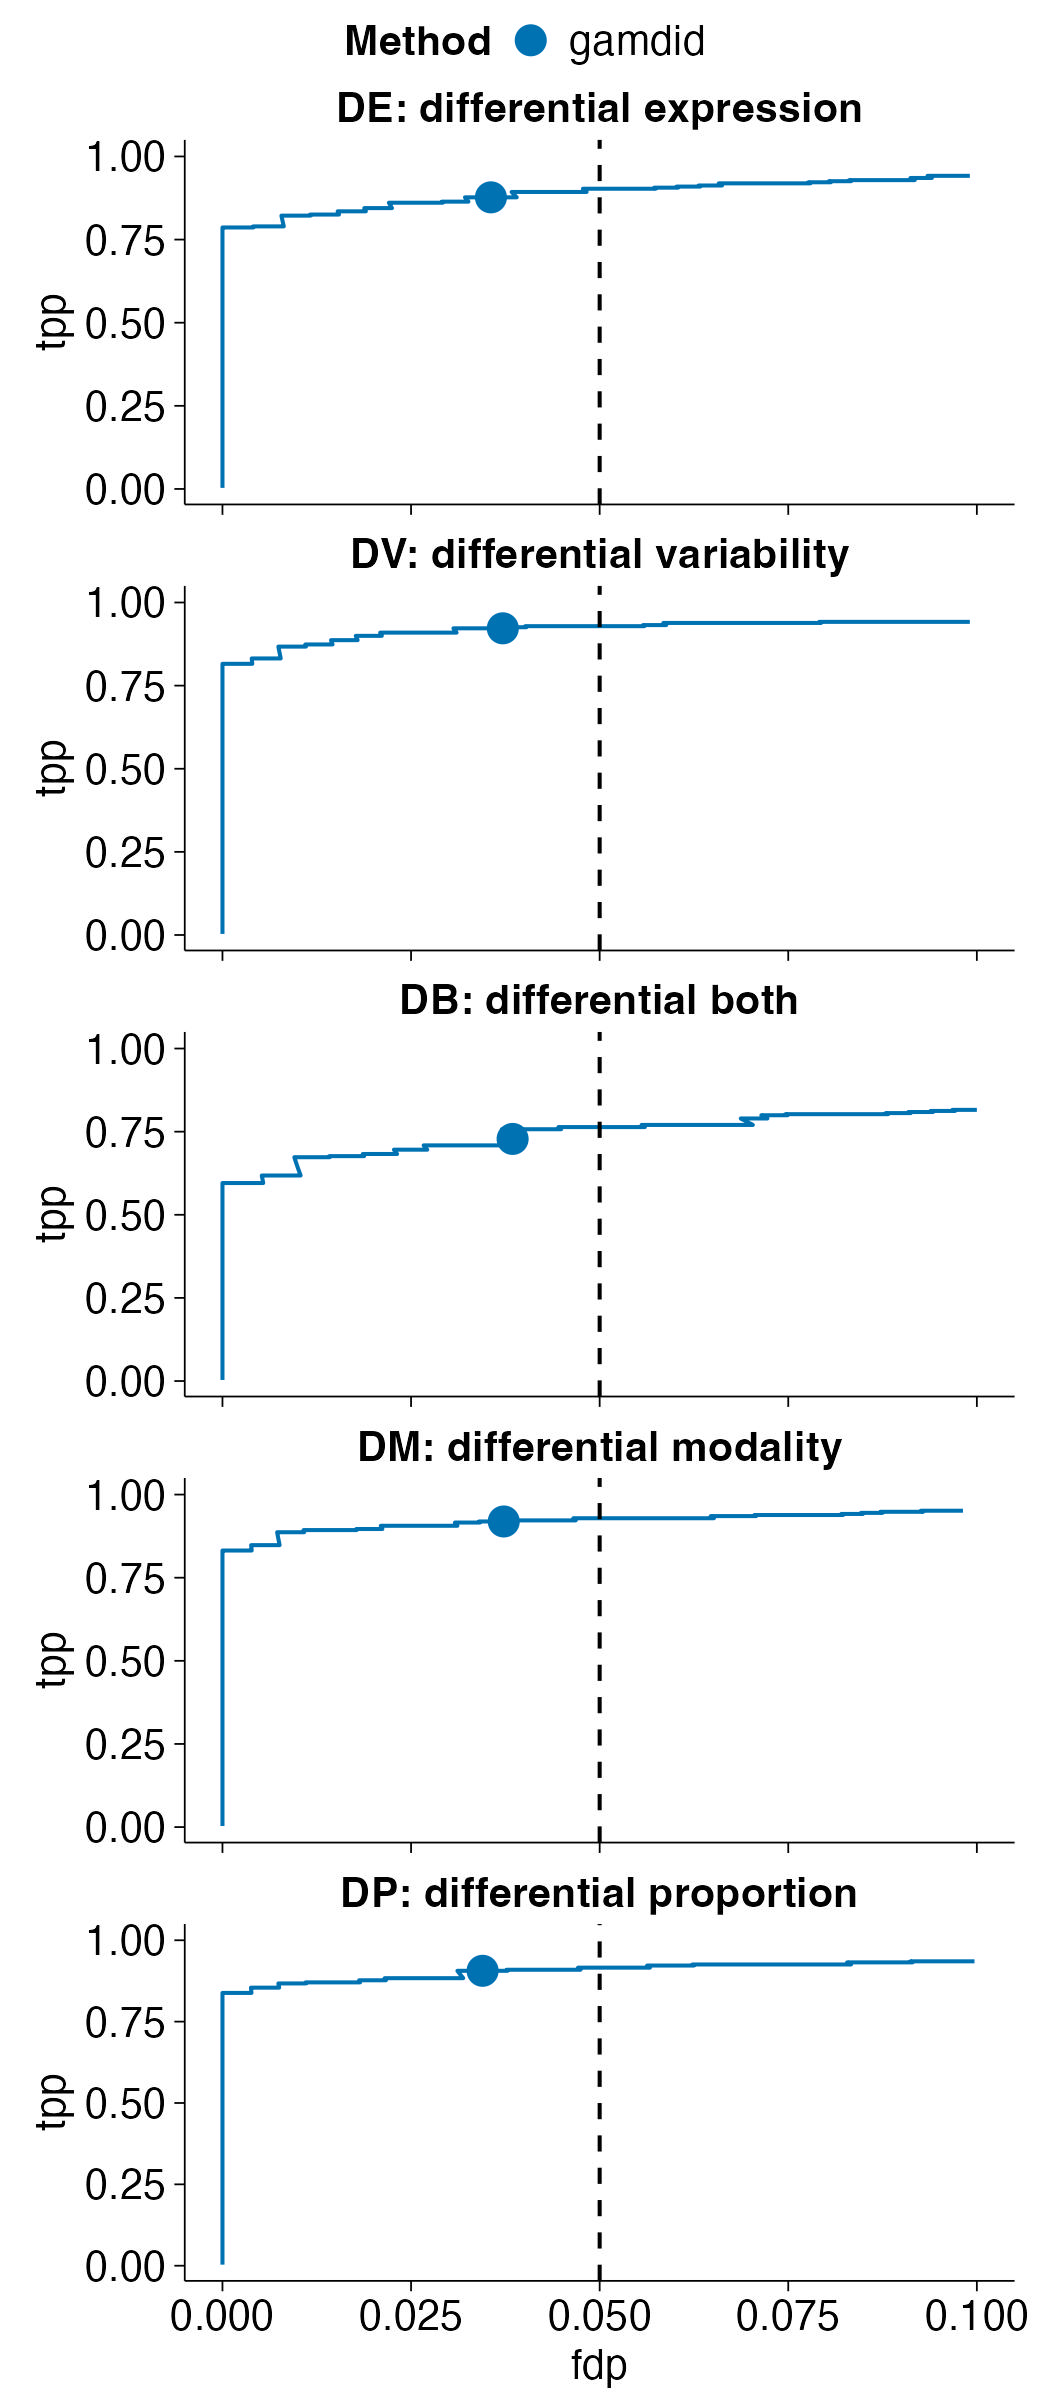
\includegraphics[width=0.425\linewidth]{figs/figS6.jpg}
    \caption{\textbf{Performance of the gamdid omnibus test in a three-group simulation} FDP-TPP curves for gamdid's omnibus test across the five simulation scenarios, based on the protein-level mock data of the Leduc dataset (755 monocytes). Cells were randomly assigned to three mock groups (A, B, C), with distributional signal introduced in group B under the same five simulation scenarios as in the two-group analyses. No competing DD method currently supports multi-group omnibus testing, so no benchmark comparison is possible here; these curves demonstrate gamdid's standalone performance in this setting. The dots mark the 5\% FDR threshold and the dashed vertical line marks FDP = 0.05. Notably, the three-group omnibus test achieves higher power than the corresponding two-group comparisons in the left column of Figure \ref{fig:leducsims_gamdid}. DB (differential both) denotes a difference in both modality and component means.}
    \label{fig:leduc_threegroup}
\end{figure}


\begin{table}[htbp]
\centering
\begin{tabular}{ccc}
\hline
\texttt{msqrob2} & \texttt{gamdid} & \texttt{distinct} \\
\hline
0.030\rlap{$^{*}$} & 0.055 & 0.039\rlap{$^{*}$}\\
0.046\rlap{$^{*}$} & 0.081 & 0.160\\
0.048\rlap{$^{*}$} & 0.081 & 0.039\rlap{$^{*}$}\\
0.048\rlap{$^{*}$} & 0.084 & 0.141\\
0.049\rlap{$^{*}$} & 0.083 & 0.055\\
0.049\rlap{$^{*}$} & 0.086 & 0.128\\
\\
0.149 & 0.090 & 0.035\rlap{$^{*}$}\\
0.128 & 0.197 & 0.039\rlap{$^{*}$}\\
\hline
\end{tabular}
\caption{\textbf{FDR-corrected p-values for features detected by msqrob2 and/or distinct but not by gamdid in the spike-in case study} The eight features that are flagged as significant by msqrob2 and/or distinct but not by gamdid are listed with their FDR-corrected p-values from all three methods. We see that gamdid consistently returns borderline non-significant p-values for the six features detected by msqrob2. In contrast, distinct produces both relatively high and relatively low p-values for these features. This indicates that only gamdid largely preserves the msqrob2 ranking of DA features. Significant FDR-corrected p-values ($<$ 0.05) are marked with an asterisk (*).}
\label{tab:only_msqrob2}
\end{table}

\begin{table}[htbp]
\centering
\begin{tabular}{ccc}
\hline
\texttt{msqrob2} & \texttt{gamdid} & \texttt{distinct} \\
\hline
0.931 & 0.028\rlap{$^{*}$} & 0.499\\
0.401 & 0.034\rlap{$^{*}$} & 0.067\\
0.074 & 0.045\rlap{$^{*}$} & 0.073\\
\hline
\end{tabular}
\caption{\textbf{FDR-corrected p-values for the three features detected exclusively by gamdid in the spike-in case study} The three features uniquely identified as significant by gamdid, with FDR-corrected p-values from all three methods. Two of the three features receive very high msqrob2 p-values, confirming that these differences do not involve a detectable mean shift and would be entirely missed by any conventional DA approach. Significant FDR-corrected p-values ($<$ 0.05) are marked with an asterisk (*).}
\label{tab:only_gamdid}
\end{table}

\clearpage
\begin{figure}[H]
    \centering
    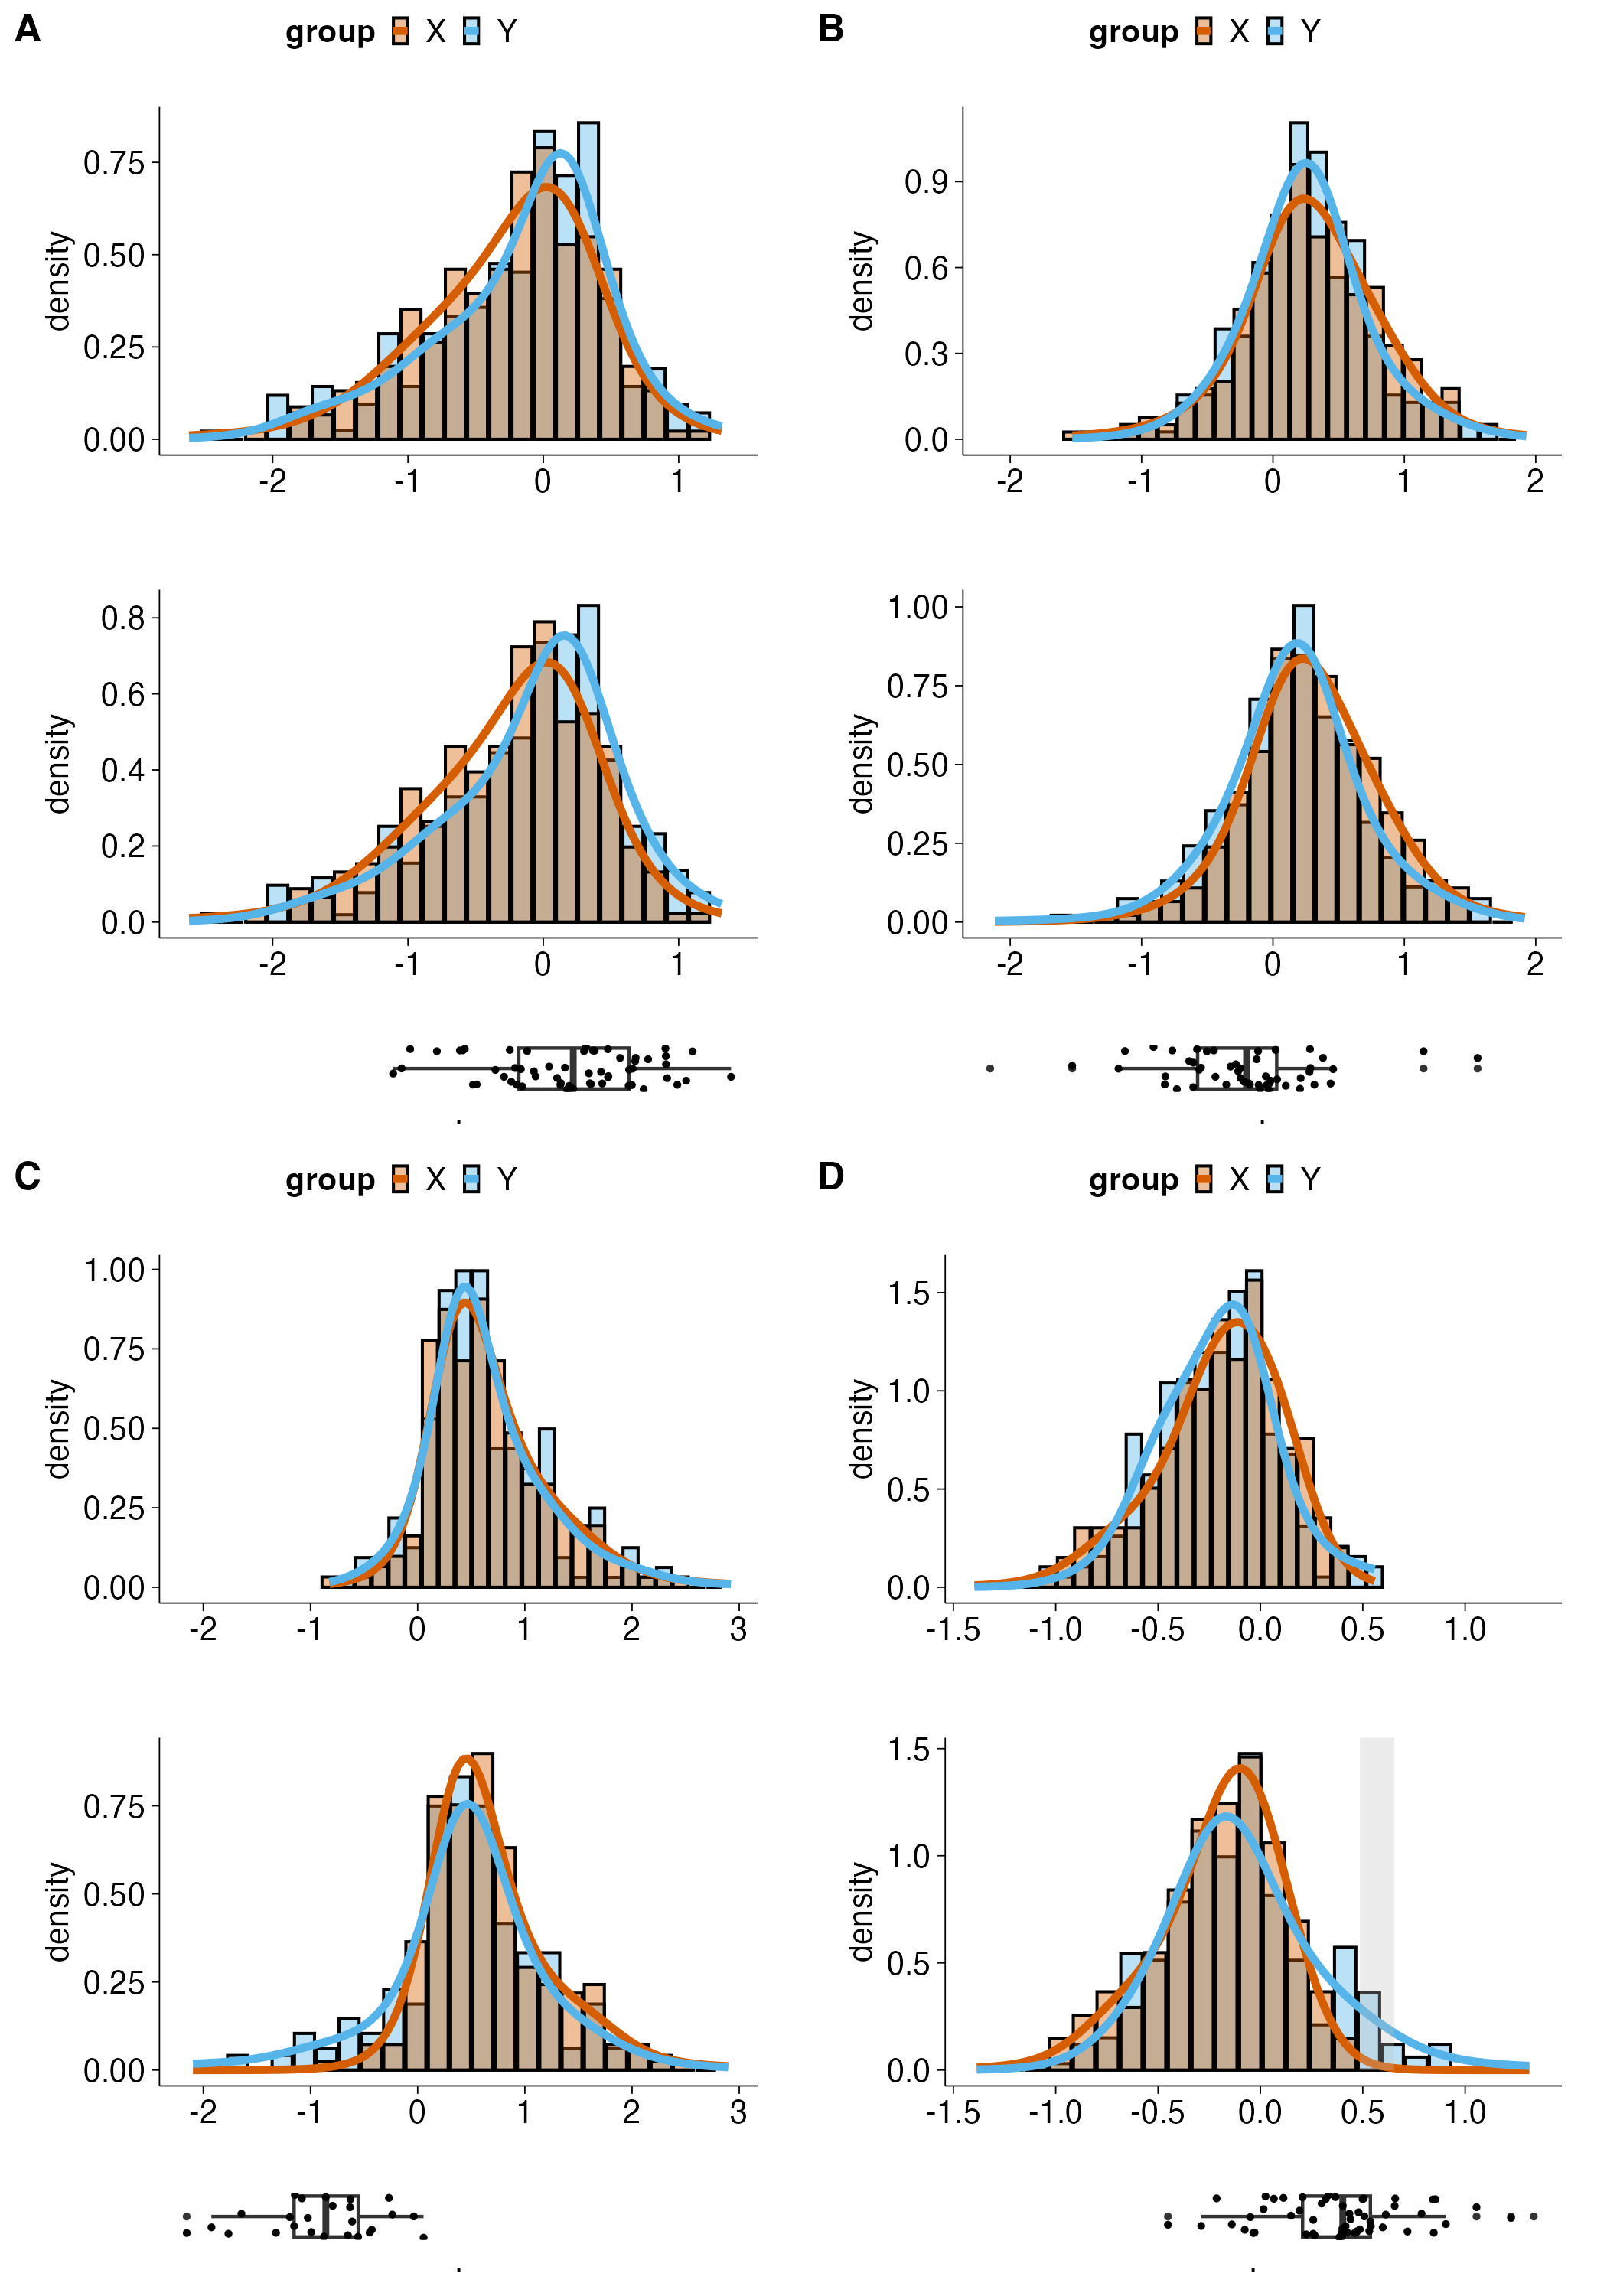
\includegraphics[width=0.85\linewidth,height=0.75\textheight,keepaspectratio]{figs/figS7.jpg}
    \captionsetup{labelfont={bf,small,color=red}}
    \caption{\textbf{\textcolor{red}{gamdid visualizations for features detected only by msqrob2 or only by distinct in the spike-in case study}} The output of gamdid's visFit function for two of the four features flagged as significant exclusively by msqrob2 (\textbf{A}, \textbf{B}) and the two features flagged as significant exclusively by distinct (\textbf{C}, \textbf{D}). Each panel shows the mock comparison (top), in which the groups show no distributional difference, the comparison after spiking 10\% of the 697 sub-cluster A melanoma cells (69 cells) into group Y (middle), and a boxplot indicating where the spike-in melanoma cells are located (bottom). \textbf{A--B}: After spike-in, a weak mean shift appears, but no differential region is found by gamdid (no gray shading). This illustrates a feature type where msqrob2's dedicated sensitivity for mean shifts gives it a slight edge over gamdid. \textbf{C}: After spike-in, the melanoma cells add a heavier left tail to the distribution of group Y, but no differential region is found by gamdid (no gray shading). Here, distinct's ECDF-based approach accumulates sufficient evidence to reach significance, while gamdid's local density approach does not identify a sufficiently concentrated differential region. \textbf{D}: After spike-in, the density of group Y shifts in the right tail, and gamdid's difference smoother identifies a differential region (gray shading), despite the FDR-corrected p-value being non-significant (gamdid FDR adjusted p-value = 0.090).}
    \label{fig:msqrob_distinct_only}
\end{figure}
\clearpage




\begin{figure}[H]
    \centering
    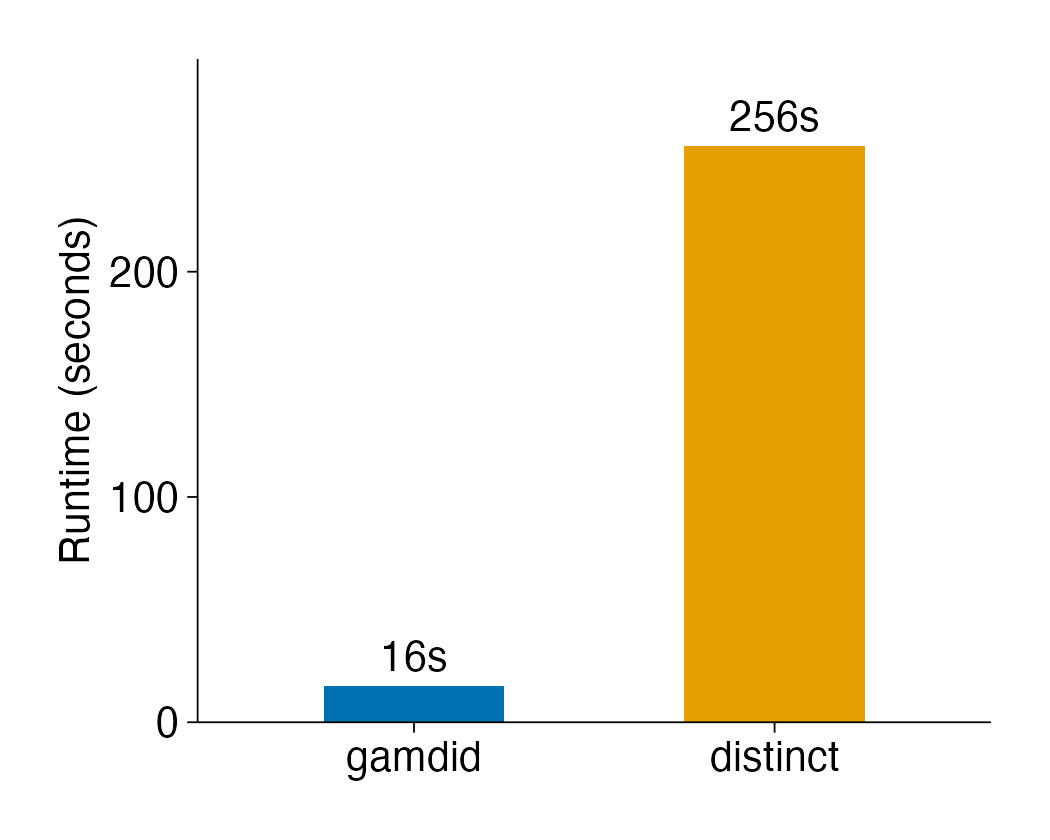
\includegraphics[width=0.425\linewidth]{figs/figS8.jpg}
    \caption{\textbf{Computational efficiency of gamdid and distinct}
    Mean runtime for gamdid and distinct on the spike-in case study dataset
    (1316 features, 824 cells), each run on a single core and averaged
    across ten independent runs. gamdid completed in 16 seconds on average,
    whereas distinct required 256 seconds, corresponding to a more than
    fifteen-fold speedup.}
  \label{fig:runtime}
\end{figure}

\subsection{\texorpdfstring{\textcolor{red}{Supplementary methods: full statistical derivation}}{Supplementary methods: full statistical derivation}} \label{suppl_methods}

\textcolor{red}{This section provides the details underlying the \texttt{gamdid} approach summarized in the Methods section.} We first detail the density estimation approach and the Poisson generalized additive model used. We subsequently describe the inference procedure and the p-value aggregation strategy. Next we elaborate on the post-hoc pairwise comparisons and stagewise testing procedure, followed by the approach for identifying regions of differential density.

\subsubsection{Model and inference}

The statistical methodology for comparing distributions is developed for a single feature (in this case proteins or peptides). The method is then simply repeated over multiple features and the corresponding p-values are corrected for multiple testing using the conventional Benjamini-Hochberg FDR procedure \cite{BH_procedure} or stagewise testing \cite{stagewise_testing}.
\\
\\
\textbf{Density estimation through Poisson regression} Following the approach of Lindsey \cite{lindsay_method}, we reformulate density estimation in terms of Poisson regression by discretizing the sample space. We partition the sample space $\mathscr{Y}$ into $K$ disjoint bins $\mathscr{Y}_k$ of equal width $bw$.

\begin{equation}
	\mathscr{Y} =\bigcup_{k=1}^K \mathscr{Y}_k
	\label{eq:discr}
\end{equation}

The data $\boldsymbol{y} = (y_1, y_2, \ldots, y_n)^T$ are summarized into bin counts $\boldsymbol{s} = (s_1, s_2, \ldots, s_K)^T$ where each count $s_k$ represents the number of observations falling into the $k$-th bin:

\begin{equation}
    s_k = \# \{ y_i \in \mathscr{Y}_k \}\quad
    \text{for } k=1,2, \ldots K
	\label{eq:binning}
\end{equation}

The sum of these counts equals the total number of observations $n$. Conceptually, this process is equivalent to constructing a histogram of the data, where each bin $\mathscr{Y}_k$ is associated with a count $s_k$ and represented by a midpoint $mid_k$.

We consider $s_k$ to be independent Poisson observations with expected values $\mu_k$

\begin{equation}
    s_k \stackrel{\text { ind }}{\sim}
    \operatorname{Po}\left(\mu_k\right) \quad
    \text{for } k=1,2, \ldots K
    \label{eq:poisson}
\end{equation}

Consequently, the problem of density estimation is recast as a spline-based Poisson regression of the bin counts $s_k$ as a function of the bin midpoints $mid_k$ \cite{efron}.
\\
\\
\textbf{Poisson generalized additive model}
The expected bin counts $\mu_k$ are modeled using Poisson regression implemented in the existing R package \texttt{mgcv} \cite{mgcv} for GAMs.

The linear predictor of a standard GAM with one smoother ($f(mid_k)$) is given by equation \ref{eq:gam}.

\begin{equation}
    g(\mu_k) = \boldsymbol{A}_k\boldsymbol{\gamma} + f(mid_k)
    \label{eq:gam}
\end{equation}

with $\boldsymbol{A}_k$ the k-th row of the parametric $K \times G$ model matrix $\boldsymbol{A}$ and $\boldsymbol{\gamma}$ the parametric part of the model parameter vector. For Poisson distributed data, the link function $g$ is a log function.

The relationship between $\log(\mu_k)$ and $mid_k$, $f(mid_k)$, is modeled using penalized thin plate regression splines (see equation \ref{eq:splines}) that provide a basis function expansion, i.e.

\begin{equation}
    f(mid_k) = \sum_{p=1}^{P}\delta_p\phi_p(mid_k)
    \label{eq:splines}
\end{equation}

where $\phi_p(.)$ are thin plate spline basis functions, $\delta_p$ are the corresponding smooth basis parameters to be estimated. Let $\boldsymbol{{\beta}} = (\boldsymbol{\gamma},\boldsymbol{\delta})$ where $\boldsymbol{\delta} = (\delta_1,\dots, \delta_P)^T$.\\
Let $\boldsymbol{\Phi}$ be the $K \times P$ model matrix of the basis functions evaluated at the midpoints: $\phi_p(mid_k)$.
We then combine $\boldsymbol{A}$ and $\boldsymbol{\Phi}$ in the $K \times (G+P)$ model matrix $\boldsymbol{X} = (\boldsymbol{A} : \boldsymbol{\Phi})$.

$\boldsymbol{\beta}$ is estimated by maximizing the penalized log-likelihood (see equation \ref{eq:beta_est})
\begin{equation}
    \hat{\boldsymbol{\beta}}=\arg \max _{\beta}\left\{l(\boldsymbol{\beta}|\boldsymbol{s})-\frac{1}{2} \lambda \boldsymbol{\beta}^{\mathrm{T}} \boldsymbol{S} \boldsymbol{\beta}\right\}
    \label{eq:beta_est}
\end{equation}

The optimization is typically performed using penalized iteratively reweighted least squares (PIRLS). Here, $l(\boldsymbol{\beta}|\boldsymbol{s})$ is the log likelihood of the data given $\boldsymbol{\beta}$, $\lambda$ is the smoothing parameter that balances goodness-of-fit with smoothness, and $\boldsymbol{S}$ is the penalty matrix quantifying the wiggliness of the basis functions that has zeros on the rows and columns involving parameters for $\boldsymbol{A}$ \cite{gambook_gamtheory_setup}. We exploit the link between Bayesian statistics, smooth functions, and mixed models to estimate this smoothing parameter $\lambda$ using the REML method \cite{gambook_gamtheory_reml, ruppert_reml}.

To approximate the effective degrees of freedom (edf) of the model, we define the influence matrix $\boldsymbol{H}$ in equation \ref{eq:infl_mat}.

\begin{equation}
    \boldsymbol{H} = (\boldsymbol{X}^T\boldsymbol{W}\boldsymbol{X} + \lambda \boldsymbol{S})^{-1}\boldsymbol{X}^T\boldsymbol{W}\boldsymbol{X}
    \label{eq:infl_mat}
\end{equation}

with $\boldsymbol{W}$ the diagonal weight matrix from the final PIRLS iteration, where $W_{kk} = \mu_k = \exp(\boldsymbol{X}_k^T \hat{\boldsymbol{\beta}})$ and $\boldsymbol{X}_k$ is the k-th row of $\boldsymbol{X}$.

In the GAM literature $2\boldsymbol{H} - \boldsymbol{H}\boldsymbol{H}$ is the bias-corrected influence matrix (the bias arises due to smoothing), so its trace can be seen as the effective degrees of freedom of the bias-corrected model (see equation \ref{eq:edf}) \cite{gambook_gamtheory_edf}.

\begin{equation}
    edf = 2\,\mathrm{tr}(\boldsymbol{H}) - \mathrm{tr}(\boldsymbol{H}\boldsymbol{H})
    \label{eq:edf}
\end{equation}
\\
\\
\textbf{Comparing distributions across groups} We build on this framework to detect distributional differences across multiple groups. Let $c$ denote a group of the grouping variable $C$.\\
Next, the overall sample space $\mathscr{Y}$ is partitioned for all groups $c$ into K disjoint bins $\mathscr{Y}_k$ of equal width $bw$ (as in equation \ref{eq:discr}), ensuring identical bins (and thus midpoints $mid_k$) for all groups $c \in C$, as illustrated in Figure \ref{fig:workflow} panel A. For each group $c$, a count vector $\boldsymbol{s_c} = (s_{c_1}, s_{c_2},...,s_{c_K})$ is obtained, where $s_{c_k}$ is the number of observations from group $c$ in the k-th bin.

The full model allows for different distributions across groups, with the linear predictor specified in equation \ref{eq:gamHa}.

\begin{equation}
    \log \mu_{ck} = \sum_{c \in C}\gamma_cx_c + \sum_{c \in C} f_c(mid_k)x_c + \log(O_c)
    \label{eq:gamHa}
\end{equation}

where each group $c$ has its own intercept $\gamma_c$ and smooth function $f_c$, with identical smoothing parameter $\lambda$ among all groups.

The offset $O_c$ is defined as

\begin{equation}
    O_c = bw \times n_c
    \label{eq:offset}
\end{equation}

where $n_c$ is the total number of observations in group $c$. This allows for normalization of different sample sizes across groups and ensures that the fitted smooth functions $\exp(\gamma_c + f_c(mid_k))$ can be directly interpreted as a probability density.

Conversely, the null model assumes a common density function across all groups of $C$. The linear predictor is modeled as in equation \ref{eq:gamH0}.

\begin{equation}
    \log \mu_{ck} = \sum_{c \in C}\gamma_cx_c + f(mid_k) + \log(O_c)
    \label{eq:gamH0}
\end{equation}

where $x_c$ is a dummy variable for the groups of covariate $C$, $\mu_{ck}$ is the expected count for group $c$ in bin $k$, and the smooth function $f(\text{mid}_k)$ is shared across all groups. $O_c$ is an offset term.
\\
\\
\textbf{Inference for distributional differences}
Two approaches were considered for testing whether distributions differ across groups.

\begin{itemize}
    \item Generalized likelihood ratio test (GLRT)
\end{itemize}
This approach is possible by comparing the full and the null model. However, it requires fitting two models and does not directly provide pairwise comparisons for a multi-group setting. Therefore, we provide a Wald-type test below and refer the reader to the GLRT section at the end of the supplementary materials.

\begin{itemize}
    \item Wald-type test
\end{itemize}

A more practical approach involves Wald-type tests on the parameters of the smooth functions of the full model (see equation \ref{eq:gamHa}). This method builds on tests proposed by Simon Wood, which assess whether a smoother significantly deviates from zero, $H_0 : f_c = 0$ \cite{Wald}.

We extend this idea to test whether multiple smooth functions are identical across $G$ groups. Specifically, we test the null hypothesis $H_0 : f_{c_1} = f_{c_2} = \dots = f_{c_G}$.
This hypothesis can be reformulated as a Wald test on the corresponding basis function parameters. Indeed, equality of smooth functions $f_{c_1} = f_{c_2} = \cdots = f_{c_G}$ implies equality of their associated parameter vectors $\boldsymbol{\beta}_{c_1} = \boldsymbol{\beta}_{c_2} = \cdots = \boldsymbol{\beta}_{c_G}$ if basis functions are shared across all groups.

To test this hypothesis, we define contrasts on the full vector of basis function parameters $\hat{\boldsymbol{\beta}}_{\text{full}} = (\hat{\boldsymbol{\beta}}_{c_1}, \dots, \hat{\boldsymbol{\beta}}_{c_G})$ from the full model in equation \ref{eq:gamHa}. The null hypothesis can then be expressed as $H_0: \boldsymbol{L}\boldsymbol{\beta}_{\text{full}} = 0$ where $\boldsymbol{L}$ is a contrast matrix encoding $G-1$ independent differences between parameter vectors, i.e. ($\boldsymbol{\beta}_{c_1} - \boldsymbol{\beta}_{c_g} = 0$ for $g = 2,\ldots,G$).\\
The corresponding Wald statistic is then given by equation \ref{eq:wald_difftest}.

\begin{equation}
    T_{W} = \hat{\boldsymbol{\beta}}_{\text{full}}^T\boldsymbol{L}^T(\boldsymbol{L}\boldsymbol{V}_{\beta_{\text{full}}} \boldsymbol{L}^T)^{-1} \boldsymbol{L}\hat{\boldsymbol{\beta}}_{\text{full}}
    \label{eq:wald_difftest}
\end{equation}

where $\boldsymbol{V}_{\beta_{\text{full}}} = (\boldsymbol{X}^T\boldsymbol{W}\boldsymbol{X} + \lambda \boldsymbol{S})^{-1}$ is the covariance matrix for $\boldsymbol{\beta}_{\text{full}}$. $T_W$ is asymptotically $\chi^2_z$ distributed.

The degrees of freedom $z$ correspond to the total edf associated with the $G-1$ smooth functions that are dropped under $H_0$.\\
%Intuitively, only one smooth function is required if $H_0$ holds, which means $G-1$ smooth functions are unnecessary and the effective degrees of freedom these smooth functions consume are essentially redundant.\\
%Consequently, $z$ is defined as the sum of the effective degrees of freedom associated with these $G-1$ smooth functions.
As a conservative estimate, we define $z$ as the sum of the $G-1$ largest edf values.

The p-value obtained from the $\chi^2_z$ distribution of $T_W$ reflects any form of distributional deviation between groups: mean shifts, differences in variance, modality, skewness, etc. In what follows, we refer to this as the GAM p-value.
\\
\\
\textbf{P-value aggregation}
While the GAM p-value is sensitive to a wide range of distributional differences, it exhibits limited power in detecting pure mean shifts. To improve sensitivity to such shifts, we complement the GAM p-value with a p-value derived from the msqrob2 framework, which is specifically designed to detect mean shifts in proteomics data using a robust linear regression through a mixed model framework \cite{msqrob}.

The GAM p-value and the msqrob2 p-value are aggregated using the HMP method. The HMP method is particularly suited for combining correlated p-values \cite{harmonicp}. This is inherently the case since mean shifts are one aspect of overall distributional changes.
The resulting aggregated p-value, termed the 'feature-level aggregated p-value', provides a single, comprehensive measure of evidence against the null hypothesis of no distributional difference among groups for that feature.
\\
\\
\textbf{Post-hoc pairwise comparisons}
If covariate $C$ comprises more than two groups, post-hoc pairwise comparisons can be conducted. For each of the $\mathcal{C}(\mathcal{C}-1)/2$ pairs of groups (where $\mathcal{C}$ is the number of groups in $C$), a pairwise GAM p-value is calculated using the Wald test framework (see equation \ref{eq:wald_difftest}) with an appropriate contrast matrix $\boldsymbol{L}$. Similarly, pairwise msqrob2 p-values are computed. These pairwise p-values are then aggregated for each group-to-group comparison using the HMP method, yielding 'pairwise aggregated p-values', each representing the evidence against the null hypothesis of identical distributions for that specific pair of groups.
\\
\\
\textbf{Stagewise testing}
A stagewise approach is employed to effectively manage the multiple hypotheses arising from feature-level and subsequent pairwise comparisons \cite{stagewise_testing}.
\begin{itemize}
    \item Stage 1 (feature-level FDR control): The feature-level aggregated p-values are adjusted across all features using the Benjamini-Hochberg (BH) procedure to control the FDR at 5\%.

    \item Stage 2 (pairwise FWER control) is only conducted if stage 1 results in a significant p-value. The pairwise aggregated p-values are adjusted for multiple testing across the $\mathcal{C}(\mathcal{C}-1)/2$ pairwise hypotheses within a feature to control the family-wise error rate (FWER) on the BH-adjusted significance level (i.e., the FDR q-value) of the first stage \cite{stager}.
\end{itemize}

%If covariate $C$ comprises two levels, only stage 1 needs to be conducted.

\subsubsection{Identifying regions of differential density}
For pairs of groups exhibiting significant distributional differences, the specific regions contributing to these differences can be pinpointed. This is achieved by constructing a difference smoother $\hat{d}$, representing the estimated difference in log-densities between the groups, and its associated simultaneous confidence bands.

Consider the comparison between two groups: $c_1$ and $c_2$ from the groups of $C$. The difference smoother $\hat{d}$ is evaluated across a grid of $N$ points: $x_n$ for $n = 1, \ldots, N$ spanning the range of $mid_k$ values (see equation \ref{eq:diffsmooth}).

\begin{equation}
\hat{d}(x_n) = (\hat{\gamma}_{c_1} + \hat{f}_{c_1}(x_n)) - (\hat{\gamma}_{c_2} + \hat{f}_{c_2}(x_n))
\label{eq:diffsmooth}
\end{equation}

Note that $\hat{d}(x_n)$ can also be expressed as a linear combination of the full parameter vector $\hat{\boldsymbol{\beta}}_{\text{full}}$. Let $\boldsymbol{x}_{diff}$ be the contrast row vector for the comparison of $c_1$ and $c_2$ so that the difference smoother can be defined as in equation \ref{eq:diffsmooth_easy}.

\begin{equation}
\hat{d}(x_n) = x_{\text{diff},n}\hat{\beta}_{\text{full}}
\label{eq:diffsmooth_easy}
\end{equation}

The corresponding pointwise standard error is subsequently computed in equation \ref{eq:diffsmooth_se}.

\begin{equation}
se(\hat{d}(x_n)) = \sqrt{x_{\text{diff,n}}^T\boldsymbol{V}_{\beta_{\text{full}}}x_{\text{diff,n}}}
\label{eq:diffsmooth_se}
\end{equation}

where $\boldsymbol{V}_{\beta_{\text{full}}}$ is the covariance matrix for $\hat{\beta}_{\text{full}}$.

A $1-\alpha$ pointwise confidence interval for $\hat{d}(x_n)$ is then given by $\hat{d}(x_n) \pm  z_{\alpha/2}\,se(\hat{d}(x_n))$ where $z_{\alpha/2}$ is the $1-\alpha/2$ quantile of the standard normal distribution.\\
To enable valid inference over the entire difference smoother $\hat{d}$ simultaneously, the pointwise confidence intervals need to be adjusted for multiple testing. Essentially, this is equivalent to adjusting for the multiple pointwise tests conducted along the grid. As a computationally efficient approach, we use the Šidák multiple testing correction to transform the pointwise intervals into simultaneous confidence bands \cite{sidak}. The Šidák correction will be conservative because the points are positively correlated \cite{simes}.\\
Regions where the simultaneous band does not encompass zero can then be used to prioritize DD regions.

The $1-\alpha_{\text{overall}}$ simultaneous confidence interval for $\hat{d}(x_n)$ then becomes $\hat{d}(x_n) \pm  z^*\,se(\hat{d}(x_n))$, where the adjusted critical value $z^*$ is $z_{1-{(1-\alpha_{\text{overall}}/2)}^{1/M}}$.
$M$ denotes the effective number of independent locations along the grid, which is conservatively estimated as the maximum of the effective degrees of freedom associated with the two smooth functions being compared $\hat{f}_{c_1}$ and $\hat{f}_{c_2}$. This choice is motivated by the equivalence between such grid tests and omnibus Wald-type tests on the basis function parameters (see equation \ref{eq:wald_difftest}).\\

Similar to the previous section, a stagewise testing approach is used to correct for multiple testing along the features. This means that $\alpha_{\text{overall}}$ corresponds to the BH adjusted significance level of the first stage to control the feature-level FDR at 5\% \cite{stagewise_testing}.\\
Note, however, that we do not provide simultaneous confidence intervals that account for multiple testing along features as well as within features to address multiple comparisons between groups. Indeed, this would require the extension of the stagewise testing procedure toward multiple stages.
%when $C$ comprises more than two levels, the differential regions are only corrected for multiple testing along the features and not along the multiple comparisons, as this would require a third stage in the stagewise testing procedure.

\subsection{Generalized likelihood ratio test} \label{suppl_glrt}

The null model (equation \ref{eq:gamH0}) can be compared to the full model (equation \ref{eq:gamHa}) using a GLRT (see equation \ref{eq:GLRT}).

\begin{equation}
    D = 2\{l(\beta_{full}) - l(\beta_{0})\}
    \label{eq:GLRT}
\end{equation}

where $l(\beta_{full})$ and $l(\beta_{0})$ are the maximized log-likelihoods for the full and the null models, respectively. Under $H_0$, $D$ asymptotically follows a chi-squared distribution (see equation \ref{eq:GLRT_distr}).

\begin{equation}
    D \sim  \chi^{2}_{\Delta \text{edf}}
    \label{eq:GLRT_distr}
\end{equation}

where $\Delta \text{edf} = \text{edf}_{full} - \text{edf}_0$. $\text{edf}_{full}$ and $\text{edf}_0$ are derived from equation \ref{eq:edf}. The p-value is then $P(\chi^2_{\Delta edf} \geq D)$ \cite{gambook_gamtheory_glrt}.\\

This approach requires fitting two models and does not directly provide pairwise comparisons if more than two groups exist.

%----------------------------------------------------------------------------------------
%	 REFERENCES
%----------------------------------------------------------------------------------------
\newpage

\printbibliography % Output the bibliography
%----------------------------------------------------------------------------------------
\end{document}
